\documentclass[11pt]{article}
\usepackage[utf8]{inputenc}
\usepackage[spanish]{babel}
\usepackage[]{graphicx}
\usepackage{colortbl} %para las tablas
\usepackage{longtable} %para las tablas
\usepackage{geometry}
\geometry{tmargin=3cm,bmargin=3cm,lmargin=3cm,rmargin=2cm}

\begin{document}

%\documentclass{article}
%
%\usepackage[spanish]{babel}
%\usepackage[utf8]{inputenc}
%\usepackage{geometry}
%\usepackage{graphicx}
%\geometry{tmargin=3cm,bmargin=3cm,lmargin=3cm,rmargin=2cm}
%
%\begin{document}

\thispagestyle{empty}
\begin{center}
\Huge{\bf{Sistema de Biblioteca Digital}}\\[5cm]

\large{\bf{
\begin{tabular}{ll}
	María Andrea Cruz Blandón. & código 0831816 \\
	Yerminson Doney Gonzalez Muñoz. & código 0843846 \\
	Cristian Leonardo Ríos López. & código 0842139 \\
	Luis Felipe Vargas Rojas. & código 0836342 \\
	Edgar Andrés Moncada Taborda. & código 0832294
\end{tabular}
}}
\end{center}

\begin{picture}(100,200)
\put(200,-100){
\includegraphics[scale=0.8]{LOGO}}
\end{picture}\\[3cm]
\begin{flushright}
\huge{Plan de Proyecto Versión 1.0}
\end{flushright}


%\end{document}
\newpage

\begin{center}
        \textbf{Resumen}
\end{center}
En el documento se observarán las siguientes secciones: Propósito, que describe como su nombre lo
indica, el propósito de este documento, Plan de proyecto, especificando que metodología se usará.\\
Alcance especifica el alcance del plan de proyecto como guía para el desarrollo del sistema de
biblioteca digital.\\
Contexto, esta sección contiene información sobre el ¿Por qué se plantea un problema?, ¿Por qué se
decide llevar a cabo esta solución? y otras cuestiones sobre el problema, esta sección está
dividida en: Planteamiento del problema y pertinencia del mismo, describe el problema que existe en
el manejo de documentos que se generan y que posee la eisc, Justificación, que describe el por qué
el sistema biblioteca digital es una buena solución para el problema que se viene presentando en la
eisc, Área de aplicación del producto resultado del proyecto incluye la aplicación del sistema
biblioteca digital en el caso particular de la universidad del valle, y Cronograma de actividades
plantea una agenda para seguirse y cumplirse para realizar todas las actividades con respecto al
desarrollo del proyecto.\\
Entre las secciones del documento seguimos con, Requerimientos, tiene como contenido los requisitos
del sistema que se han planteado por parte de Marta Millán y Mauricio Gaona, esta sección se divide
en: Descripción del sistema, explica a grandes rasgos y con enfoque de requisitos el sistema
biblioteca digital, Visión y alcance, esta sección explica de manera mucho más profunda el sistema
biblioteca digital, al igual que descripción del sistema, mantiene un enfoque de requisitos,
Usuarios, contiene información detallada sobre los usuarios del sistema biblioteca digital, esta es una de las secciones importantes puesto que en adelante se referirán a algunos actores con nombres de usuarios descritos aquí, Matriz de requerimientos, es la matriz que contiene todos los
requerimientos que se han identificado y Descripción detallada, cada requerimiento de la matriz de
requerimientos es pasado a una plantilla de documento que describe mas profundamente el
requerimiento, esto con el fin de eliminar ambigüedades.\\
Lo siguiente corresponde a la sección de Análisis esta contiene: Descripción del subsistema, se
plantea el procedimiento a seguir con las iteraciones, Diagrama de casos de uso, contiene
precisamente toda la información y gráficos sobre los diagramas de casos de uso, esta sección se
divide a su vez en Especificación de casos de uso donde justamente se toma cada uno de los casos de
usos graficados y se llevan a una plantilla de documento donde se explicará el flujo normal y
alternativo por si lo tiene, además pre y post condiciones.\\
Finalmente tenemos la sección de Referencias donde se listan todos los documentos que se
necesitaron tener en cuenta para la realización de este plan de proyecto.

\newpage
\tableofcontents
\newpage
        
\section{Propósito}
El propósito del Sistema Biblioteca Digital es ofrecer al público en general el acceso a los
diferentes documentos digitales que se producen por el trabajo en conjunto de profesores y
estudiantes de últimos semestres en la Escuela de Ingeniería de Sistemas y Computación (EISC) de la
Universidad del Valle.
Los diferentes documentos digitales son tesis o trabajos de grados presentados por los estudiantes
y notas de clase, artículos y resultados de trabajos en la escuela producto de los profesores.
El desarrollo nace de la necesidad de poder tener esta información al servicio de lo estudiantes,
profesores y personas en general interesadas en el área de las ciencias de la computación.

\section{Alcance}
El Sistema de Biblioteca Digital solicitado por Martha Millán  y Mauricio Gaona representantes de
la EISC, abarcara solo los documentos que se produzcan en la Escuela y que pertenezcan a las áreas
de las Ciencias de la Computación. Estos documentos estarán al alcancé de los estudiantes y
profesores, además de cualquier persona que desee registrarse en el sistema y esté interesado en
los documentos. 
El Sistema de Biblioteca Digital permitirá el manejo  y gestión de usuarios, además de permitir el
catalogo de los diferentes documentos para su consulta y posterior descarga.

\section{Contexto}
        \subsection{Planteamiento del problema y pertinencia del mismo}
        Cada día dentro de la escuela de ingeniería de sistemas se generan producciones académicas 			por parte de estudiantes y profesores, producciones que de alguna manera no se almacenan
        correctamente en algunos casos, sobre todo, las producciones digitales que a pesar de que
        fueron presentadas en ciertas circunstancias importantes no son del conocimiento de todos o
        no están al alcance de todos porque no se pensó que el tema podría llegar a ser de interés
        general. Por esta razón se cree que mantener la información en un solo lugar para que esta
        pueda ser usada en algún momento como herramienta en la formación académica de los 
        estudiantes y profesores se convirtió en un problema que buscamos afrontar y solucionar de
        la mejor manera, intentando beneficiar a todas las personas involucradas e interesadas en
        el.
        El problema nos muestra como se maneja ineficientemente los documentos en la escuela de
        ingeniería de sistemas y computación, es por esta razón que de alguna manera la solución de
        este nos permitirá tener un mejor acceso a la información según nuestro intereses y de esta
        forma ayudar a que el conocimiento dentro de la escuela de ingeniería de sistemas pueda ser
        accedido, compartido, analizado y estudiado por muchas mas personas permitiendo ampliar de
        manera cómoda las formas de pensar y el conocimiento sin sufrir por la búsqueda de 
        información.
        
        \subsection{Objetivo}
        Desarrollar una aplicación para una biblioteca digital que permita reunir de manera
        organizada un conjunto de documentos que han sido producidos en el área de ciencias de la
        computación a lo largo del tiempo y que son de utilidad para la escuela de ingeniería de
        sistemas de la universidad del valle. La aplicación permitirá a lo usuarios realizar
        consultas sobre documentos almacenados y si se registran tendrán la posibilidad de
        descargarlo y usarlo como complemento en su aprendizaje. Lo que se busca es poder manejar
        la información generada de manera centralizada y ordenada lo que permitirá un excelente
        control sobre ellos y su rápida ubicación. Posteriormente, con la aplicación se podrán
        generar estadísticas que muestren el trabajo realizado por el sistema y como esto a
        aportado a los usuarios una mejor manera de consultar información.
        De este modo vemos que el camino que deseamos seguir implica mejorar el                      
        conocimiento de cada una de de las personas implicadas y la manera en que estas               
        obtiene información sobre este tipo de áreas.        
        
        \subsection{Justificación}
        La escuela de ingeniería de sistemas y computación se ve con la necesidad de organizar los
        documentos que produce, con ciertas características facilitando la búsqueda, también
        necesita de un sistema que integre a los usuarios interesados para que además de poder
        consultar documentos puedan descargarlos, logrando una retroalimentación mucho mas marcada
        que con la organización actual de documentos donde no están disponibles para todos los
        interesados. por otro lado se debe seguir estadística sobre esta información para realizar
        análisis sobre los contenidos.
        Es por todo lo anterior que el planteamiento del sistema biblioteca digital, ofrece una
        solución que satisface todas esas necesidades, y que se presenta como un sistema práctico y
        accesible a todos los interesados por los documentos de las ciencias de la computación.
        
        \subsection{Área de aplicación}
        El área institucional sobre todo para instituciones educativas en este caso la universidad
        del valle la cual tiene personas dentro de su campus que están interesadas en temas 
        relacionados con ciencias de la computación y que serian beneficiados de gran manera por
        ese sistema.
        
        \subsection{Cronograma de actividades}
        \begin{minipage}[c]{1\linewidth}
                \centering
                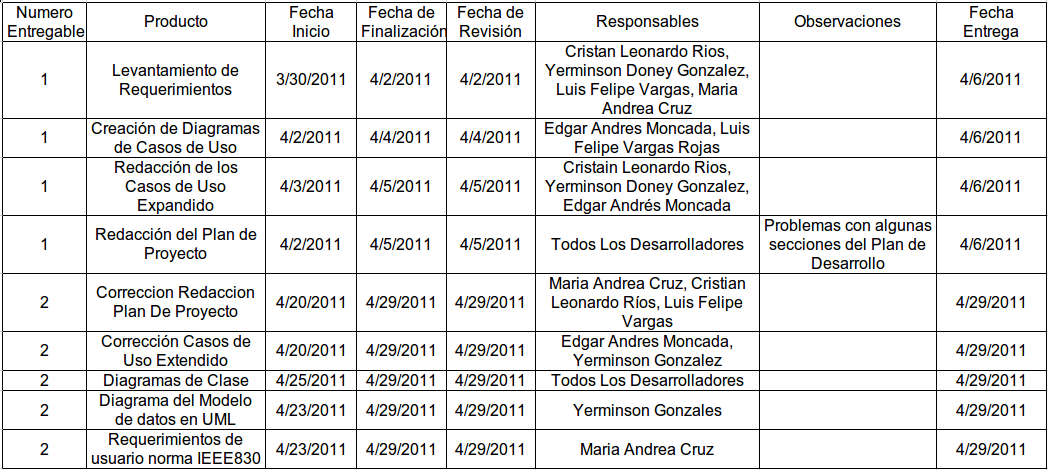
\includegraphics[width=16cm, height=9cm]{Cronograma2}
        \end{minipage}
        
\section{Requerimientos}
        \subsection{Descripción del sistema}
        El sistema busca tener agrupados y organizados los documentos creados y que posee la
        escuela de ingeniería de sistemas y computación (eisc), teniendo en cuenta, los metadatos
        que el catalogador le otorgue a cada documento y las áreas de interés. Con el fin de tener
        a disposición de la comunidad de la eisc y de interesados en los documentos de las ciencias
        de la computación.
        
        El sistema correrá en un equipo como aplicación de escritorio, que este conectado a 
        internet para acceder a la base de datos, donde se encontrarán alojados toda la información
        de documentos y usuarios.
        
        \subsection{Visión y alcance}
        El proyecto tiene como fin la elaboración del sistema biblioteca digital solicitado por los
        profesores y representantes de la dirección de la EISC Marta Millan y Mauricio Gaona para
        la poner a la disposición de los interesados en las ciencias de computación los diferentes
        tipos de documentos que se producen en la Escuela por Estudiantes y Docentes.
        
        Los objetivos principales del sistema son:
        
        \textbf{La gestión de usuarios:} incluye los tipo de usuario registrado y no registrado.
        Para los registrados se administraran con 3 perfiles de usuarios a los cuales se les otorga
        ciertos permisos. El administrador que gestiona las operaciones y la información 
        relacionada con los demás usuarios, asignar los perfiles y los demás permisos. El 
        catalogador que se le otorga los permisos de catalogación de los documentos digitales. Y
        por ultimo los usuarios normales y los anteriores que podrán consultar y descargar
        documentos. Se almacenaran para los usuarios registrados datos personales, sobre áreas de 
        interés y demográficos.
        
        \textbf{La catalogación de los documentos:} los diferentes documentos se almacenaran con 
        los diferentes metadatos para su consulta. Se debe guardar datos como autor, área a la que 
        pertenece, datos básicos y palabras claves.
        
        \textbf{La generación de Reportes:} Es necesario hacer un seguimiento, a las consultas,
        catalogaciones y descargas de documentos por lo que el sistema debe generar reportes en 
        formato PDF que contengan esta información.
        
                \subsubsection{Entregables}
                \textbf{Primer Entregable:} En el primer entregable se inicion las fases Inicio y
                Elaboración de la metodología RUP. En este entregable se incluyen:
                
                \begin{itemize}
                \item\textbf{Plan del proyecto:} es este documento, que consigna el plan global a
                seguirpara el desarrrollo del sistema biblioteca digital.
                \item\textbf{Matriz de Requerimientos y descripción detallada:} Comprende los
                requisitos del sistema especificados por los stakeholders y el documento del
                planteamiento del problema.
                Se presenta una matriz que contiene identificación de los requerimientos,
                descripción, fuente, prioridad, estado e involucrados. A cada requerimiento se le
                realiza una descripción detallada usando una plantilla de documento en donde además
                de los datos anteriores de la matriz incluye requerimientos asociados, datos salida
                y resultados esperados.
                \item\textbf{Diagrama de Casos de uso:} Corresponde a la representación gráfica de
                los actores y sus relaciones con las funciones del sistema.
                \item\textbf{Casos de uso expandido:} Son las especificaciones de los casos de uso,
                se realiza por cada caso de uso usando la plantilla de documento que incluye los
                campos precondiciones, flujo normal, flujo alternativo, postcondiciones y 
                excepciones.
                \end{itemize}
                
                \textbf{Segundo Entregable:} Aqui se se refinan fases inicio y elaboración y se
                inicia fase de construcción.
                
                \begin{itemize}
                \item\textbf{Plan de proyecto:} Refinamiento del primer entregable, y adición de
                algunos apartes.
                \item\textbf{Diagrama de casos de uso:} Refinamiento del primer entregable.
                \item\textbf{Casos de uso expandido:} Refinamiento del primer entregable.
                \item\textbf{Requerimientos de usuario norma IEEE830:} Documento que especifica la
                buena obtención de requisitos de sotfware de manera que el cliente conozca bien que
                es lo que desea del sistema, y que los desarrrolladores sepan que es lo que deben
                realizar, tratando de preveer malas estimaciones de tiempo y recursos.
                \end{itemize}
                
                \textbf{Tercer Entregable:} Se refinan fases inicio, elaboracion y construcción y
                se adicionan artefactos a la fase de construcción.
                
                \begin{itemize}
                \item\textbf{Plan de proyecto:} Refinamiento del segundo entregable.
                \item\textbf{Diagrama de casos de uso:} Refinamiento del segundo entregable.
                \item\textbf{Casos de uso expandido:} Refinamiento del segundo entregable.
                \item\textbf{Requerimientos de usuario norma IEEE830:} Refinamiento del segundo
                entregable.
                \item\textbf{Diagrama del modelo de datos en UML:} Debido a que el sistema
                biblioteca digital hace uso de una base de datos, este diagrama tiene el modelo
                Entidad Relacion y Relacional haciendo uso de un profile UML para modelado de
                datos.
                \item\textbf{Diagrama de clases:} Modelo estático que describirá la estructura del
                sistema biblioteca digital mostrando sus clases, atributos y relaciones entre
                ellas, la primera versión de este diagrama de clases esta sujeta a modificaciones
                conforme el proyecto avance y se realicen iteraciones en la fase de construcción.
                Estarán contenidos en el aprate Analisis del plan de proyecto.
                \item\textbf{Diagrama de paquetes:} muestra cómo el sistema biblioteca digital está
                dividido en agrupaciones lógicas mostrando las dependencias entre esas
                agrupaciones. se presenta de modo modular y denotan una jerarquía. Este diagrama
                permite un mejor acoplamiento a nivel externo.
                \item\textbf{Diagramas de secuencia:} En estos diagramas se mostrara la interacción
                de los diferentes objetos del sistema a través del tiempo. Se modelán para cada
                caso de uso, por lo que para este artefacto los casos de uso deben estar lo
                suficientemente desarrrollados y refinados.
                \item\textbf{Prototipos interfaz de usuario:} Serán unos prototipos creados con
                herramientas para graficos y otros interactivos con el fin de obtener
                retroalimentación de los stakeholders con respecto a los requerimientos, así ellos
                tendrán un adelanto de lo que será la interfaz del sistema.
                \item\textbf{Modelo de implementación inicial:} Se establece estructura para la
                implementación inicial, concretando manejo de ejecutables, ajustes de subsistemas
                de implementación. Se establecen responsables y módulos para la integración.
                \end{itemize}
                
                \textbf{Cuarto Entregable:} Aqui se realizan los ultimos refinamientos de las fases
                inicio, elaboración y construcción y se inicia fase de transacción.
                
                \begin{itemize}
                \item\textbf{Plan de proyecto:} Refinamiento del tercer entregable.
                \item\textbf{Diagrama de casos de uso:} Refinamiento del tercer entregable.
                \item\textbf{Casos de uso expandido:} Refinamiento del tercer entregable.
                \item\textbf{Requerimientos de usuario norma IEEE830:} Refinamiento del tercer
                entregable.
                \item\textbf{Diagrama del modelo de datos en UML:} Refinamiento del tercer
                entregable.                
                \item\textbf{Diagrama de clases:} Refinamiento del tercer entregable.
                \item\textbf{Diagrama de paquetes:} Refinamiento del tercer entregable.
                \item\textbf{Diagramas de secuencia:} Refinamiento del tercer entregable.
                \item\textbf{Prototipos interfaz de usuario:} Refinamiento del tercer entregable.
                \item\textbf{Casos de pruebas:} Usando plantilla de documento, se establecen los
                casos de pruebas, describiendo entradas de la prueba, y salidas esperadas, también
                procedimiento para realizar las pruebas. Dependiendo del tipo de prueba podrán ser
                o no automatizables. 
                \item\textbf{Diagramas de despliegue:} Se utiliza para modelar el hardware 
                utilizado en las implementaciones de sistemas y las relaciones entre sus
                componentes.                
                \item\textbf{Material de apoyo al usuario final:} Documentos para el usuario final
                que corresponden a las especificaciones para hacer uso del sistema biblioteca
                digital y ayuda para el usuario.
                \item\textbf{Modelo de implementacion final:} Producto.
                \end{itemize}
                
                \subsubsection{Involucrados}
                Las personas involucradas en el desarrollo del sistema biblioteca digital son los
                representantes de la eisc Martha Millán y Mauricio Gaona, y los desarrolladores del
                proyecto Yerminson Doney Gonzalez Muñóz, Cristian Leonardo Ríos López, Edgar Andrés
                Moncada Taborda, Luis Felipe Vargas Rojas y María Andrea Cruz Blandón.
                
        \subsection{Usuarios}
        \textbf{Usuario normal:} el usuario normal de el sistema tendrá la posibilidad de consultar
        documentos , descargar documentos , solicitar notificaciones de novedades de ciertas áreas
        además de modificar algunos de sus datos.
        
        \textbf{Catalogador:} que a su ves es un usuario normal tendrá la capacidad de catalogar
        documentos lo que incluye subir documentos , además de añadir palabras claves y nuevas
        áreas de ciencias de la computación al sistema.
        
        \textbf{Administrador:} podrá hacer cambios de perfiles a los usuario el sistema, también
        podrá borrar usuarios, y cambiar datos de los mismos.
        
		\subsection{Matriz de requerimientos}
               %\documentclass[10pt,a4paper]{article}
%
%
%\usepackage[spanish]{babel}
%\usepackage[utf8]{inputenc}
%\usepackage{geometry}
%\usepackage{colortbl}
%
%\geometry{tmargin=1cm,bmargin=2cm,lmargin=2cm,rmargin=2cm}
%\begin{document}
\begin{center}
\begin{longtable}{|p{0.5cm}|p{3cm}|p{2cm}|p{0.8cm}|p{1.5cm}|p{2cm}|}

\hline
\multicolumn{6}{|>{\columncolor[rgb]{0.8,0.8,0.8}}c|}{ MATRIZ DE REQUERIMIENTOS  }\\
\hline
\multicolumn{6}{|p{12cm}|}{Aclaración: Los requerimientos que están en color rojo, son requerimientos que  no se alcanzaron a implementar}\\
\hline
\bf {id} &\bf { Descripción} & \bf {Fuente} & \bf {Prio.} &\bf { Estado} & \bf {Usuarios involucrados}\\

\hline

R2
&	

Proporcionar un perfil  a cada usuario
&	

Marta Millán y Mauricio Gaona.
&	

media
&	

Revisión
	
&
Catalogador, administrador.\\
\hline
R3
&	

Modificar datos de usuarios
&	

Marta Millán y Mauricio Gaona.
&	

baja
&	

Revisión
&	

Catalogador, usuario normal, administrador\\
\hline
R4
&	

Eliminar usuario.
&	

Marta Millán, Mauricio Gaona.
&	

baja
&	

Revisión
&	

Administrador\\
\hline
R5
&	

Enviar notificación a los usuarios de nuevos documentos registrados en un area de su interes.
&	

Marta Millán y Mauricio Gaona.
&	

media
&	

Revisión
&	

Catalogador, usuario normal, administrador.\\
\hline
R6
&	

autenticar el login y la contraseña del usuario a ingresar.
&	

Marta Millán y Mauricio Gaona.
&	

media
&	

Revisión
&	

Catalogador, usuario normal, administrador.\\
\hline					

R7
&	

Almacenar los Documentos Digitales para su descarga.
&	

Marta Millán y Mauricio Gaona.
&	

alta
&	

Revisión
&	

Catalogador,  Administrador\\
\hline
R8
&	

Catalogar documentos añadiendo meta-datos
&	

Marta Millán y Mauricio Gaona.
&	

alta
&	

Revisión
&	

Catalogador\\
\hline
R9
&	

Modificar meta-datos de documentos
&	

Marta Millán y Mauricio Gaona.
&	

media
&	

Revisión
&	

Catalogador\\
\hline
R10
&	

Eliminar documentos y la información relacionada con ellos.
&	

Marta Millán y Mauricio Gaona.
&	

media
&	

Revisión
&	

Administrador, catalogador\\
\hline
R11
&

Permitir el almacenamiento, y modificación de información de  documentos solo a administradores y catalogadores.
&	

Marta Millán y Mauricio Gaona.
&	

media
&	

Revisión
&	

Administrador,

catalogador\\
\hline

R12
	
&
Clasificar documentos por áreas de interés.
&	

Marta Millán y Mauricio Gaona.
&	

media
&	

Revisión
&	

Catalogador\\
\hline

R13
&	

Permitir solo a los catalogadores y el Administrador clasificar documentos.
&	

Marta Millán y Mauricio Gaona.
&	

media
&	

Revisión
&	

Catalogador, Administrador\\
\hline
R14	
&
Almacenar meta-datos de los autores de los documentos presentes en el sistema.
&	

Marta Millán y Mauricio Gaona.
&	

media
&	

Revisión
&	

Catalogador, Administrador\\

\hline
R15
&	

Almacenar un nuevo autor y modificar información sobre autores existentes.
&	

Marta Millán y Mauricio Gaona.
&	

media
&	

Revisión
&	

Catalogador, Administrador\\
\hline
R16
&	

Añadir palabras claves a documentos almacenados en la BD.
&	

Marta Millán y Mauricio Gaona.
&	

media
&	

Revisión
&	

Catalogador, Administrador\\
\hline
R17
&	

Crear nuevas palabras claves añadiendo su descripción .
&	

Marta Millán y Mauricio Gaona.
&	

media
&	

Revisión
&	

Catalogador, Administrador\\
\hline
R18
&	

Almacenar áreas de interés con sus respectivas subáreas.
&	

Marta Millán y Mauricio Gaona.
&	

media
&	

Revisión
&	

Catalogador\\
\hline
R19
&	

Permitir modificar y eliminar áreas de interés solo por parte de administradores y catalogadores.
&	

Marta Millán y  Mauricio Gaona.
&	

media
&	

Revisión
&	

Catalogador, y administrador.\\
\hline
R20
	&

Permitir el registro de nuevas áreas
	&	
 Marta Millán y  Mauricio Gaona.

 &
media
	&

Revisión
	&

Catalogador y Administrador\\
					
\hline
R21
	
&
Permitir la consulta básica de documentos.
&	

Marta Millán y Mauricio Gaona.
&	

alta
&	

Revisión
&	

Usuarios normales registrados o no registrados, catalogador y administrador. \\
\hline
R22
&	

Permitir la consulta avanzada de documentos.
&	

Marta Millán y Mauricio Gaona.
&	

alta
&	

Revisión
&	

Usuarios normales registrados o no registrados, catalogador y administrador.\\
\hline

R23
	&

Permitir la descarga de documentos.
	&

Marta Millán y  Mauricio Gaona.
	&

alta
	&

Revisión
	&

Usuarios Registrados, catalogadores y administrador.\\
\hline
R24
	&

Listar nombre de documento y su correspondiente autor como resultado de una consulta
	&

Marta Millán y Mauricio Gaona.
	&

media
	&

Revisión
	&

Usuarios  registrados o no registrados, catalogador y administrador.\\
\hline
R25
&	

Mostrar ficha técnica de un documento.
&	

Marta Millán y Mauricio Gaona.
&	

media
&	

Revisión
&	

Usuarios normales registrados o no registrados, catalogador y administrador.\\

\hline
R26
&	

Generar reportes en formato PDF de los documentos descargasdos por fecha.
&	

Marta Millán y Mauricio Gaona.
&	

media
&	

Revisión
&	

Administrador.\\
\hline
R27
	&

Generar reportes en formato PDF de los documentos descargados por área
	&

Marta Millán y Mauricio Gaona.
	&

media
	&

Revisión
	&

Administrador.\\
\hline
R28
&	

Generar reportes en formato PDF de los documentos existentes por área
&	

Marta Millán y Mauricio Gaona.
&	

media
&	

Revisión
&	

Administrador.\\
\hline
R29
&	

Generar reportes en formato PDF de los documentos existentes por autor
&	

Marta Millán y Mauricio Gaona.
&	

media
&	

Revisión
&	

Administrador.\\
\hline
R30
&	

Generar reportes en formato PDF del total de usuarios registrados.
&	

Marta Millán y Mauricio Gaona.
&	

media
&	

Revisión
&	

Administrador.\\
\hline
R31
&	

Generar reportes en formato PDF del total de usuarios registrados por fecha.
&	

Marta Millán y Mauricio Gaona.
&	

media
&	

Revisión
&	

Administrador.\\
\hline
R32
	&

Generar reportes en formato PDF de las consultas por fecha.
	&

Marta Millán y Mauricio Gaona.
	&

media
	&

Revisión
	&

Administrador.\\
\hline
R33
	&

Generar reportes en formato PDF de las consultas por área.
	&

Marta Millán y Mauricio Gaona.
	&

media
	&

Revisión
	&

Administrador.\\
\hline
R34
	&

Generar reportes en formato PDF de los documentos catalogados por fecha.
	&

Marta Millán y Mauricio Gaona.
	&

media
	&

Revisión
	&

Administrador.\\
\hline
R35
	&

Generar reportes en formato PDF de los documentos descargados por usuario.
	&

Marta Millán y Mauricio Gaona
	&

media
	&

Revisión
	&

Administrador.\\
\hline
R36
	
&
Generar reportes en formato PDF de los documentos existentes por tipo de documento.
&	

Marta Millán y Mauricio Gaona
&	

media
&	

Revisión
&	

Administrador.\\
\hline
R37
	&

Generar reportes en formato PDF de los documentos existentes por formato.
	&

Marta Millán y Mauricio Gaona
	&

media
	&

Revisión
	&

Administrador.\\
\hline
R38
	&

Generar reportes en formato PDF de los documentos catalogados por área.
	&

Marta Millán y Mauricio Gaona
	&

media
	&

Revisión
	&

Administrador.\\
\hline


\end{longtable}
\end{center}

%\end{document} 
                %\pagebreak        
        
        \subsection{Descripción detallada}
                %\documentclass[]{article}
%\usepackage[spanish]{babel}
%\usepackage[utf8]{inputenc}
%\usepackage{geometry}
%\usepackage{colortbl}
%\usepackage{longtable}
%\geometry{tmargin=3cm,bmargin=3cm,lmargin=3cm,rmargin=2cm}
%\begin{document}
%para incluir comentar hasta acá
\begin{center}
\begin{longtable}{|p{0.225\textwidth}|p{0.225\textwidth}|p{0.225\textwidth}|p{0.225\textwidth}|}
\hline
\multicolumn{2}{|p{0.45\textwidth}|}{{\bf {Función del requerimiento:}}
Permitir el registro de nuevos usuarios. } & {\bf{ Estado}} & Análisis \\
\hline
\multicolumn{2}{|p{0.45\textwidth}}{\bf Identificador} &
\multicolumn{2}{|p{0.45\textwidth}|}{R01} \\
\hline
\multicolumn{2}{|p{0.45\textwidth}}{\bf {Tipo de requerimiento}} &
\multicolumn{2}{|p{0.45\textwidth}|}{Funcional}\\
\hline
\bf {Creado por} & María Andrea Cruz & \bf {Fecha } & Marzo 31 2011 \\
\hline
\bf {Actualizado por} & Felipe Vargas & \bf {Fecha }& Abril 02 2011\\
\hline
\bf {Actualizado por} & Cristian Ríos & \bf {Fecha }& Mayo 09 2011\\
\hline
\bf Descripción &\multicolumn{3}{p{0.675\textwidth}|}
{El sistema después de que el usuario proporcione los datos correspondiente (login, contraseña, pregunta secreta, respuesta secreta, nombres, apellidos, género, fecha de nacimiento, correo electrónico, nivel de escolaridad, vínculo con Univalle, áreas de interés.) los almacenará en la base de datos. El usuario pasará a ser un usuario registrado, con acceso al sistema mediante logueo.} \\
\hline
\bf Datos de entrada &\multicolumn{3}{p{0.675\textwidth}|}{
Para que un usuario se registre debe de proporcionar obligatoriamente un login, una contraseña, una pregunta secreta, una respuesta secreta a la pregunta, su primer nombre, su primer apellido, su género y correo electrónico. Opcionalmente puede proporcionar el segundo nombre, el segundo apellido, la fecha de nacimiento, el nivel de escolaridad, el vínculo con univalle y sus área de conocimiento de interés.}\\
\hline
\bf Datos de salida &\multicolumn{3}{p{0.675\textwidth}|}
{Un mensaje que informa al usuario que el registro se ha dado de manera exitosa y que puede loguearse de ahora en adelante formando parte de los usuarios registrados.} \\
\hline
\bf Resultados esperados &\multicolumn{3}{p{0.675\textwidth}|}
{El sistema deberá realizar una modificación en la base de datos de usuarios lo que permite que en un futuro sea reconocido.} \\
\hline
\bf Origen &\multicolumn{3}{p{0.675\textwidth}|}
{Documento de descripción del problema.} \\
\hline
\bf Dirigido a &\multicolumn{3}{p{0.675\textwidth}|}
{Estudiantes , profesores , funcionarios de Univalle y administrador} \\
\hline
\bf Prioridad &\multicolumn{3}{p{0.675\textwidth}|}{5} \\
\hline
\bf Requerimientos Asociados &\multicolumn{3}{p{0.675\textwidth}|}
{} \\
\hline
\multicolumn{4}{|>{\columncolor[rgb]{0.8,0.8,0.8}}c|}{\bf Especificación}\\
\hline
\bf Precondiciones &\multicolumn{3}{p{0.675\textwidth}|}
{El sistema debe estar conectado a la base de datos, la interfaz debe corresponder a la de usuario no registrado, es decir, la inicial.} \\
\hline
\hline
\bf Poscondicion &\multicolumn{3}{p{0.675\textwidth}|}
{El sistema tiene un nuevo usuario que se ve especificado como un nuevo registro en la base de datos en lo que corresponde a usuarios. } \\
\hline
\bf Criterios de Aceptación &\multicolumn{3}{p{0.675\textwidth}|}
{El requerimiento es aceptado si es posible registrarse como usuario en el sistema Biblioteca Digital.} \\
\hline
\end{longtable}
\end{center}
%\end{document} %comentar para inlcuir
                %%\pagebreak
                
                %\documentclass[]{article}
%\usepackage[spanish]{babel}
%\usepackage[utf8]{inputenc}
%\usepackage{geometry}
%\usepackage{colortbl}
%\usepackage{longtable}
%\geometry{tmargin=3cm,bmargin=3cm,lmargin=3cm,rmargin=2cm}
%\begin{document}
%para incluir comentar hasta acá
\begin{center}
\begin{longtable}{|p{0.225\textwidth}|p{0.225\textwidth}|p{0.225\textwidth}|p{0.225\textwidth}|}
\hline
\multicolumn{2}{|p{0.45\textwidth}|}{{\bf {Función del requerimiento:}}
Proporcionar un perfil a cada usuario. } & {\bf{ Estado}} & Análisis \\
\hline
\multicolumn{2}{|p{0.45\textwidth}}{\bf Identificador} &
\multicolumn{2}{|p{0.45\textwidth}|}{R02} \\
\hline
\multicolumn{2}{|p{0.45\textwidth}}{\bf {Tipo de requerimiento}} &
\multicolumn{2}{|p{0.45\textwidth}|}{Funcional}\\
\hline
\bf {Creado por} & María Andrea Cruz & \bf {Fecha } & Marzo 31 2011 \\
\hline
\bf {Actualizado por} & Cristian Ríos & \bf {Fecha }& Abril 28 2011\\
\hline
\bf {Actualizado por} & Cristian Ríos & \bf {Fecha } & Mayo 09 2011\\


\hline
\bf Descripción &\multicolumn{3}{p{0.675\textwidth}|}
{El sistema debe proporcionar un perfil a cada usuario, esto aplica a los usuarios que ya están registrados, es decir, se encuentran en la base de datos, esta acción es gestionada por el administrador. Por defecto todo usuario registrado tiene como perfil ‘Usuario Normal’} \\
\hline
\bf Datos de entrada &\multicolumn{3}{p{0.675\textwidth}|}{
Para poder asignar un perfil a cada usuario se presentan al administrador todos los datos del usuario a modificar de manera informativa para verificar la identidad del usuario. El administrador debe de proporcionar el dato perfil con el que se le realizará la actualización al usuario.}\\
\hline
\bf Datos de salida &\multicolumn{3}{p{0.675\textwidth}|}
{El administrador recibe una mensaje notificando el éxito o no de la operación y el usuario implicado recibe una notificación de su cambio de estado en el sistema.} \\
\hline
\bf Resultados esperados &\multicolumn{3}{p{0.675\textwidth}|}
{El sistema deberá actualizar la base de datos permitiendo al usuario que se le a actualizado su perfil tener nuevas funcionalidades en el sistema.} \\
\hline
\bf Origen &\multicolumn{3}{p{0.675\textwidth}|}
{Documento de descripción del problema.} \\
\hline
\bf Dirigido a &\multicolumn{3}{p{0.675\textwidth}|}
{Catalogador, administrador y usuarios normales.} \\
\hline
\bf Prioridad &\multicolumn{3}{p{0.675\textwidth}|}{3} \\
\hline
\bf Requerimientos Asociados &\multicolumn{3}{p{0.675\textwidth}|}
{\begin{itemize}
        \item R06
\end{itemize} } \\
\hline
\multicolumn{4}{|>{\columncolor[rgb]{0.8,0.8,0.8}}c|}{\bf Especificación}\\
\hline
\bf Precondiciones &\multicolumn{3}{p{0.675\textwidth}|}
{El sistema debe estar conectado a una base de datos, un administrador debe haberse logueado en el sistema lo que permite privilegios en cuanto al cambio de perfil de otros usuarios.} \\
\hline
\hline
\bf Poscondicion &\multicolumn{3}{p{0.675\textwidth}|}
{El sistema de ahora en adelante reconoce al usuario modificado en su perfil de manera diferente, otorgándole determinados privilegios así como su interfaz de usuario correspondiente.} \\
\hline
\bf Criterios de Aceptación &\multicolumn{3}{p{0.675\textwidth}|}
{El requerimiento es aceptado si cada usuario que se registre tiene como perfil 'Usuario Normal' y si posteriormente, un usuario administrador puede actualizar el perfil del usuario a 'Catalogador' o 'Administrador'.}
\\
\hline
\end{longtable}
\end{center}
%\end{document} %comentar para inlcuir
                %%\pagebreak
                
                %\documentclass[10pt,a4paper]{article}
%
%
%\usepackage[spanish]{babel}
%\usepackage[utf8]{inputenc}
%\usepackage{geometry}
%\usepackage{colortbl}
%\usepackage{longtable}
%
%\geometry{tmargin=1cm,bmargin=2cm,lmargin=2cm,rmargin=2cm}
%\begin{document}
\begin{center}


\begin{longtable}{|p{3cm}|p{3cm}|p{3cm}|p{3cm}|}

\hline
\multicolumn{2}{|p{6cm}|}{{\bf {Descripción del requerimiento:}}
    Modificar datos de usuario.  } & 
     {\bf{ Estado:}} & Análisis \\
\hline
\bf {Creado por:} & 
	Maria Andrea Cruz   & \bf {Actualizado por:} & Felipe Vargas  \\
\hline
\bf {Fecha Creación } & Marzo 31 2011 & \bf {Fecha de  Actualización }& Abril 2 del 2011\\
\hline 
\multicolumn{2}{|p{6cm}|}{\bf Identificador} & \multicolumn{2}{|p{6cm}|}{R03} \\
\hline
\bf {Tipo de requerimiento:} & No Crítico &  \bf{Tipo de requerimiento:} & Funcional\\     
\hline
\bf Descripción &\multicolumn{3}{|p{10cm}|}
{ El sistema debe proporcionar una opción que permita modificar algunos de  los datos que el usuario registró, para saber que datos modificar lo hace a partir de una consulta a la base de datos que le informe el contenido actual de cada uno de los campos.} \\
\hline
\bf Datos de salida &\multicolumn{3}{|p{10cm}|}
{ El sistema actualiza en la base de datos lo referente a los atributos de usuario y se informa al usuario de la operación exitosa.} \\
\hline
\bf resultados esperados &\multicolumn{3}{|p{10cm}|}
{El sistema se ve estimulado con un cambio en la base de datos con nueva información actualizada y correcta del usuario que solicito esta funcionalidad. } \\
\hline
\bf Origen &\multicolumn{3}{|p{10cm}|}{Documento de descripción del problema.} \\
\hline
\bf Dirigido a  &\multicolumn{3}{|p{10cm}|}
{Catalogador, administrador y usuarios normales.} \\
\hline
\bf Prioridad &\multicolumn{3}{|p{10cm}|}{3} \\
\hline
\bf Requerimientos Asociados &\multicolumn{3}{|p{10cm}|}
{\begin{itemize}
	\item R06
\end{itemize} } \\
\hline
\multicolumn{4}{|>{\columncolor[rgb]{0.8,0.8,0.8}}c|}{\bf Especificación}\\
\hline


\bf Precondiciones &\multicolumn{3}{|p{10cm}|}
{El sistema debe estar conectado a la base de datos de la misma manera debe de haber reconocido a un usuario normal es decir este debe de estar logueado y observando su determinada interfaz correspondiente a su perfil.} \\
\hline
\hline
\bf Poscondiciones &\multicolumn{3}{|p{10cm}|}
{El sistema en la base de datos tiene información actualizada de acuerdo a la los datos que modifico el usuario. Lo que permite una mejor comunicación sistema usuario.} \\
\hline
\bf Criterios de Aceptación &\multicolumn{3}{|p{10cm}|}
{Criterio de aceptación del requerimiento} \\
\hline

\end{longtable}
\end{center}

%\end{document} 
                %%\pagebreak
                
                %\documentclass[]{article}
%\usepackage[spanish]{babel}
%\usepackage[utf8]{inputenc}
%\usepackage{geometry}
%\usepackage{colortbl}
%\usepackage{longtable}
%\geometry{tmargin=3cm,bmargin=3cm,lmargin=3cm,rmargin=2cm}
%\begin{document}
%para incluir comentar hasta acá
\begin{center}
%caluculado sobre el 90%, con 100% no queda bien
%lo que se debe cambiar es lo que esta en MAYUSCULA
\begin{longtable}{|p{0.225\textwidth}|p{0.225\textwidth}|p{0.225\textwidth}|p{0.225\textwidth}|}
\hline
\multicolumn{2}{|p{0.45\textwidth}|}{{\bf {Descripción del requerimiento:}}
Eliminar usuarios. } & {\bf{ Estado}} & Análisis \\
\hline
\bf {Creado por} & Maria Andrea Cruz & \bf {Actualizado por} & Cristian Ríos \\
\hline
\bf {Fecha Creación } & Marzo 31 2011 & \bf {Fecha de Actualización }& Abril 28 2011\\
\hline
\multicolumn{2}{|p{0.45\textwidth}}{\bf Identificador} &
\multicolumn{2}{|p{0.45\textwidth}|}{R04} \\
\hline
\multicolumn{2}{|p{0.45\textwidth}}{\bf {Tipo de requerimiento}} &
\multicolumn{2}{|p{0.45\textwidth}|}{Funcional}\\
\hline
\bf Descripción &\multicolumn{3}{p{0.675\textwidth}|}
{ El sistema debe proporcionar a los usuarios administradores una
opción que permita eliminar lógicamente usuarios registrados, esto es, se
le cambiará su estado a 'deshabilitado' lo que impedirá que ingrese al
sistema, restringiendo así sus funcionalidades dentro del mismo. Los
usuarios que se desea eliminar se seleccionan a partir de una lista
creada por una consulta a la base de datos que muestre el o los posibles
usuarios a eliminar.} \\
\hline
\bf Datos de salida &\multicolumn{3}{p{0.675\textwidth}|}
{ El sistema genera y muestra un mensaje de confirmación preguntando al administrador si está totalmente seguro de realizar dicha operación, de ser así, genera y muestra un mensaje informando del éxito o no de la operación solicitada.} \\
\hline
\bf Resultados esperados &\multicolumn{3}{p{0.675\textwidth}|}
{ El sistema deberá realizar una actualización del estado del usuario o los usuarios eliminados en la base de datos.} \\
\hline
\bf Origen &\multicolumn{3}{p{0.675\textwidth}|}
{Documento de descripción del problema.} \\
\hline
\bf Dirigido a &\multicolumn{3}{p{0.675\textwidth}|}
{Administrador.} \\
\hline
\bf Prioridad &\multicolumn{3}{p{0.675\textwidth}|}{3} \\
\hline
\bf Requerimientos Asociados &\multicolumn{3}{p{0.675\textwidth}|}
{\begin{itemize}
        \item R06
\end{itemize}} \\
\hline
\multicolumn{4}{|>{\columncolor[rgb]{0.8,0.8,0.8}}c|}{\bf Especificación}\\
\hline
\bf Precondiciones &\multicolumn{3}{p{0.675\textwidth}|}
{El sistema debe estar conectado a la base de datos , un administrador debe estar logueado para poder tener acceso a la interfaz de eliminación de usuarios proporcionada por el sistema.} \\
\hline
\bf Poscondicion &\multicolumn{3}{p{0.675\textwidth}|}
{El sistema en caso de tener éxito en la acción eliminar, actualiza en su base de datos los registros de los usuarios indicados para ser eliminados , por lo cual, el usuario ya no podrá ingresar al sistema.} \\
\hline
\bf Criterios de Aceptación &\multicolumn{3}{p{0.675\textwidth}|}
{El requerimiento es aceptado si un usuario administrador puede buscar posibles usuarios a eliminar y de estos seleccionar los que desee para posteriormente eliminarlos, además, el usuario eliminado le será imposible ingresar al sistema.} \\
\hline
\end{longtable}
\end{center}
%\end{document} %comentar para inlcuir
                %\pagebreak
                
                %\documentclass[]{article}
%\usepackage[spanish]{babel}
%\usepackage[utf8]{inputenc}
%\usepackage{geometry}
%\usepackage{colortbl}
%\usepackage{longtable}
%\geometry{tmargin=3cm,bmargin=3cm,lmargin=3cm,rmargin=2cm}
%\begin{document}
%para incluir comentar hasta acá
\begin{center}
\begin{longtable}{|p{0.225\textwidth}|p{0.225\textwidth}|p{0.225\textwidth}|p{0.225\textwidth}|}
\hline
\multicolumn{2}{|p{0.45\textwidth}|}{{\bf {Descripción del requerimiento:}}
Enviar notificación a los usuarios de nuevos documentos registrados en un área de su interés. } & {\bf{ Estado}} & Análisis \\
\hline
\bf {Creado por} & María Andrea Cruz & \bf {Actualizado por} & Cristian Ríos \\
\hline
\bf {Fecha Creación } & Marzo 31 2011 & \bf {Fecha de Actualización }& Abril 28 de 2011\\
\hline
\multicolumn{2}{|p{0.45\textwidth}}{\bf Identificador} &
\multicolumn{2}{|p{0.45\textwidth}|}{R05} \\
\hline
\multicolumn{2}{|p{0.45\textwidth}}{\bf {Tipo de requerimiento}} &
\multicolumn{2}{|p{0.45\textwidth}|}{Funcional}\\
\hline
\bf Descripción &\multicolumn{3}{p{0.675\textwidth}|}
{El sistema debe proporcionar a cada usuario una notificación cuando este ingrese la siguiente vez al sistema de los nuevos documentos que hayan sido catalogados en un área en la que el usuario haya mostrado interés. } \\
\hline
\bf Datos de salida &\multicolumn{3}{p{0.675\textwidth}|}
{El sistema informará al usuario de los nuevos documentos que ahora se encuentran en su área de interés. } \\
\hline
\bf Resultados esperados &\multicolumn{3}{p{0.675\textwidth}|}
{El sistema deberá realizar notificaciones a los usuarios y estos a partir de las notificaciones empiezan a consultar y descargar los nuevos documentos. El sistema no presenta ningún cambio de estado.} \\
\hline
\bf Origen &\multicolumn{3}{p{0.675\textwidth}|}
{Documento de descripción del problema} \\
\hline
\bf Dirigido a &\multicolumn{3}{p{0.675\textwidth}|}
{Catalogador, administrador y usuarios normales.} \\
\hline
\bf Prioridad &\multicolumn{3}{p{0.675\textwidth}|}{4} \\
\hline
\bf Requerimientos Asociados &\multicolumn{3}{p{0.675\textwidth}|}
{\begin{itemize}
        \item R07
        \item R08
\end{itemize}
} \\\hline
\multicolumn{4}{|>{\columncolor[rgb]{0.8,0.8,0.8}}c|}{\bf Especificación}\\
\hline
\bf Precondiciones &\multicolumn{3}{p{0.675\textwidth}|}
{El sistema debe tener acceso a la base de datos para establecer que usuarios tiene como áreas de interés las que corresponden a los nuevos documentos catalogados.} \\
\hline
\bf Poscondicion &\multicolumn{3}{p{0.675\textwidth}|}
{Se podréa ver un aumento en la cantidad de consultas para el documento catalogado ya que los usuarios han sido notificados y empezarán a consultar estos nuevos documentos.} \\
\hline
\bf Criterios de Aceptación &\multicolumn{3}{p{0.675\textwidth}|}
{El requerimiento es aceptado si a los usuarios registrados que muestren preferencia por alguna área del conocimiento se les notifica de nuevos documentos catalogados en estas áreas.} \\
\hline
\end{longtable}
\end{center}
%\end{document} %comentar para inlcuir
                %%\pagebreak
                
                %\documentclass[]{article}
%\usepackage[spanish]{babel}
%\usepackage[utf8]{inputenc}
%\usepackage{geometry}
%\usepackage{colortbl}
%\usepackage{longtable}
%\geometry{tmargin=3cm,bmargin=3cm,lmargin=3cm,rmargin=2cm}
%\begin{document}
%para incluir comentar hasta acá
\begin{center}
\begin{longtable}{|p{0.225\textwidth}|p{0.225\textwidth}|p{0.225\textwidth}|p{0.225\textwidth}|}
\hline
\multicolumn{2}{|p{0.45\textwidth}|}{{\bf {Descripción del requerimiento:}}
Verificar el logueo de usuarios. } & {\bf{ Estado}} & Análisis \\
\hline
\multicolumn{2}{|p{0.45\textwidth}}{\bf Identificador} &
\multicolumn{2}{|p{0.45\textwidth}|}{R06} \\
\hline
\multicolumn{2}{|p{0.45\textwidth}}{\bf {Tipo de requerimiento}} &
\multicolumn{2}{|p{0.45\textwidth}|}{Funcional}\\
\hline
\bf {Creado por} & Maria Andrea Cruz & \bf {Fecha } & Marzo 31 2011 \\
\hline
\bf {Actualizado por} & María Andrea & \bf {Fecha }& Abril 28 2011\\
\hline
\bf {Actualizado por} & Cristian Ríos & \bf {Fecha }& Mayo 09 2011\\
\hline
\bf Descripción &\multicolumn{3}{p{0.675\textwidth}|}
{ El sistema debe proporcionar la autenticación de cualquier usuario que se encuentre registrado y desee ingresar al sistema, esto se logra realizando una consulta a la base de datos con el nombre de usuario proporcionado por el usuario, si existe el usuario en la base de datos el resultado de la consulta será la contraseña, la cual se comparará con la proporcionada por el usuario, si ambas coinciden entonces se le otorgará al usuario el acceso al sistema.} \\
\hline
\bf Datos de entrada &\multicolumn{3}{p{0.675\textwidth}|}{
El usuario debe de proporcionar su login y su contraseña para tener acceso al sistema.}\\
\hline
\bf Datos de salida &\multicolumn{3}{p{0.675\textwidth}|}
{ El sistema permite al usuario ingresar al sistema mostrando la interfaz de su respectivo perfil.} \\
\hline
\bf Resultados esperados &\multicolumn{3}{p{0.675\textwidth}|}
{ El deberá cambiar la interfaz del usuario permitiéndole nuevas funcionalidades como por ejemplo opciones de descarga de documentos.} \\
\hline
\bf Origen &\multicolumn{3}{p{0.675\textwidth}|}
{Documento de descripción del problema.} \\
\hline
\bf Dirigido a &\multicolumn{3}{p{0.675\textwidth}|}
{Catalogador, administrador y usuarios normales.} \\
\hline
\bf Prioridad &\multicolumn{3}{p{0.675\textwidth}|}{5} \\
\hline
\bf Requerimientos Asociados &\multicolumn{3}{p{0.675\textwidth}|}
{\begin{itemize}
        \item R01
\end{itemize}} \\\hline
\multicolumn{4}{|>{\columncolor[rgb]{0.8,0.8,0.8}}c|}{\bf Especificación}\\
\hline
\bf Precondiciones &\multicolumn{3}{p{0.675\textwidth}|}
{El sistema debe estar conectado a la base de datos ya que debe reconocer que el usuario esta registrado realizando una consulta a esta a partir de los datos suministrados en la interfaz de login.} \\
\hline
\hline
\bf Poscondicion &\multicolumn{3}{p{0.675\textwidth}|}
{El sistema debe de mostrar una nueva interfaz para el usuario lo que indica que este proceso se realizó satisfactoriamente, en caso de no lograrlo se le seguirá solicitando que realice el proceso de loguin si quiere acceder a nuevas funcionalidades.} \\
\hline
\bf Criterios de Aceptación &\multicolumn{3}{p{0.675\textwidth}|}
{El requerimiento se acepta cuando un usuario registrado ingresando los datos correctos de login y password pueda ingresar al sistema; y cuando se presente impedimento para ingresar al sistema cuando los datos sean incorrectos} \\
\hline
\end{longtable}
\end{center}
%\end{document} %comentar para inlcuir
                %%\pagebreak
                
                %%\documentclass[letter]{article}
%\usepackage[spanish]{babel}
%\usepackage[utf8]{inputenc}
%\usepackage{geometry}
%\usepackage{colortbl}
%\usepackage{longtable}
%\geometry{tmargin=3cm,bmargin=3cm,lmargin=3cm,rmargin=2cm}
%\begin{document}
%para incluir comentar hasta acá
\begin{center}
\begin{longtable}{|p{0.225\textwidth}|p{0.225\textwidth}|p{0.225\textwidth}|p{0.225\textwidth}|}
\hline
\multicolumn{2}{|p{0.45\textwidth}|}{{\bf {Descripción del requerimiento:}}
Almacenar documentos digitales. } & {\bf{ Estado}} & Análisis \\
\hline
\bf {Creado por} & Maria Andrea Cruz & \bf {Actualizado por} & Cristian Ríos \\
\hline
\bf {Fecha Creación } & Marzo 31 2011 & \bf {Fecha de Actualización }& Abril 28 2011\\
\hline
\multicolumn{2}{|p{0.45\textwidth}}{\bf Identificador} &
\multicolumn{2}{|p{0.45\textwidth}|}{R07} \\
\hline
\multicolumn{2}{|p{0.45\textwidth}}{\bf {Tipo de requerimiento}} &
\multicolumn{2}{|p{0.45\textwidth}|}{Funcional}\\
\hline
\bf Descripción &\multicolumn{3}{p{0.675\textwidth}|}
{ El sistema debe de proporcionar la manera de almacenar persistentemente los documentos que vayan apareciendo para la biblioteca digital, los documentos almacenados tiene una ruta en el sistema operativo host y esta ruta será almacenada en la base de datos con algunos otros datos asociados al documento. Esta operación podrá ser ejecutado por usuarios que tengan como perfil administrador o catalogador.
} \\
\hline
\bf Datos de salida &\multicolumn{3}{p{0.675\textwidth}|}
{ El sistema genera un mensaje notificando al usuario que este solicitando la operación el éxito o no de esta.} \\
\hline
\bf Resultados esperados &\multicolumn{3}{p{0.675\textwidth}|}
{ El sistema deberá almacenar de manera persistente el documento requerido y la ruta de este en la base de datos.} \\
\hline
\bf Origen &\multicolumn{3}{p{0.675\textwidth}|}
{Documento de descripción del problema.} \\
\hline
\bf Dirigido a &\multicolumn{3}{p{0.675\textwidth}|}
{Catalogador, administrador.} \\
\hline
\bf Prioridad &\multicolumn{3}{p{0.675\textwidth}|}{5} \\
\hline
\bf Requerimientos Asociados &\multicolumn{3}{p{0.675\textwidth}|}
{\begin{itemize}
        \item R08
\end{itemize}} \\\hline
\multicolumn{4}{|>{\columncolor[rgb]{0.8,0.8,0.8}}c|}{\bf Especificación}\\
\hline
\bf Precondiciones &\multicolumn{3}{p{0.675\textwidth}|}
{El sistema debe tener acceso a la base de datos y haberse logueado en él un usuario cuyo perfil sea adminsitrador o catalogador, este usuario deberá disponer de una interfaz que permita introducir información relativa al documento como lo es su lugar de origen. } \\
\hline
\hline
\bf Poscondicion &\multicolumn{3}{p{0.675\textwidth}|}
{El sistema guarda el documento en el disco duro y el registro en la base de datos mostrando una notificación de lo realizado. } \\
\hline
\bf Criterios de Aceptación &\multicolumn{3}{p{0.675\textwidth}|}
{El requerimiento es aceptado si un usuario administrador o catalogador ingresa al sistema y logra  subir un nuevo documento a la biblioteca digital.} \\
\hline
\end{longtable}
\end{center}
%\end{document} %comentar para inlcuir
                %%\pagebreak
                
                %\documentclass[]{article}
%\usepackage[spanish]{babel}
%\usepackage[utf8]{inputenc}
%\usepackage{geometry}
%\usepackage{colortbl}
%\usepackage{longtable}
%\geometry{tmargin=3cm,bmargin=3cm,lmargin=3cm,rmargin=2cm}
%\begin{document}
%para incluir comentar hasta acá
\begin{center}
\begin{longtable}{|p{0.225\textwidth}|p{0.225\textwidth}|p{0.225\textwidth}|p{0.225\textwidth}|}
\hline
\multicolumn{2}{|p{0.45\textwidth}|}{{\bf {Descripción del requerimiento:}}
Catalogar documentos. } & {\bf{ Estado}} & Análisis \\
\hline
\bf {Creado por} & Maria Andrea Cruz & \bf {Actualizado por} & Maria Andrea Cruz \\
\hline
\bf {Fecha Creación } & Mayo 08 2011 & \bf {Fecha de Actualización }& Mayo 09 2011\\
\hline
\multicolumn{2}{|p{0.45\textwidth}}{\bf Identificador} &
\multicolumn{2}{|p{0.45\textwidth}|}{R08} \\
\hline
\multicolumn{2}{|p{0.45\textwidth}}{\bf {Tipo de requerimiento}} &
\multicolumn{2}{|p{0.45\textwidth}|}{Funcional}\\
\hline
\bf Descripción &\multicolumn{3}{p{0.675\textwidth}|}
{El sistema debe de proporcionar la posibilidad a los usuarios que tengan como perfil catalogador o administrador de catalogar documentos, esto es, copiar un nuevo documento al repositorio del sistema y asignarle datos que lo identifiquen en el mismo, estos datos son información sobre el documento como el autor, el titulo principal, el título secundario o traducido, la editorial, la fecha de publicación, la fecha de creación, el idioma en el que esta escrito, los derechos de autor, la descripción o resumen del material, las palabras claves relacionadas con este, el área de las ciencias de la computación a la que pertenece, el formato del archivo, el tamaño del archivo en bytes, la resolución en píxeles y el software recomendado para abrir el documento. Para copiar el documento al repositorio el usuario debe de indicar cual es la ruta actual del documento en el sistema host.} \\
\hline
\bf Datos de entrada &\multicolumn{3}{p{0.675\textwidth}|}{
El usuario que este realizando la operación de catalogación debe de proporciona de manera obligatoria los siguientes datos sobre el documento: el título principal, el idioma en el que esta escrito el documento, la descripción del documento, el formato, el elnace  a donde se encuentra actualmente el documento, el o los autores del documento, las palabras clave relacionadas con el documento, la o las áeras de las ciencias de la computación a la que pertence, los derechos de autor, la editorial, la fecha de publicación y el tipo al que pertenece el documento. Puede proporcinar además el título secundario o traducido, la fecha de creación, el tamaño del archivo en bytes, la resolución en pixeles(si aplica) y el software recomendado para abrir el documento. }\\
\hline
\bf Datos de salida &\multicolumn{3}{p{0.675\textwidth}|}
{ Se informa al usuario que solicitó la catalogación del documento éxito o no de la operación.} \\
\hline
\bf Resultados esperados &\multicolumn{3}{p{0.675\textwidth}|}
{ El sistema deberá realizar actualizaciones en la base de datos creando nuevos registros en las tablas que mantienen la información de los documentos con la información proporcionada por el usuario.} \\
\hline
\bf Origen &\multicolumn{3}{p{0.675\textwidth}|}
{Documento de descripción del problema.} \\
\hline
\bf Dirigido a &\multicolumn{3}{p{0.675\textwidth}|}
{Catalogador, administrador.} \\
\hline
\bf Prioridad &\multicolumn{3}{p{0.675\textwidth}|}{3} \\
\hline
\bf Requerimientos Asociados &\multicolumn{3}{p{0.675\textwidth}|}
{\begin{itemize}
        \item R06
        \item R17
        \item R14
        \item R18
\end{itemize}} \\\hline
\multicolumn{4}{|>{\columncolor[rgb]{0.8,0.8,0.8}}c|}{\bf Especificación}\\
\hline
\bf Precondiciones &\multicolumn{3}{p{0.675\textwidth}|}
{El sistema debe estar conectado a la base de datos y tener logueado a un usuario con los perfiles correspondientes a administrador o catalogador los cuales tienen acceso a una interfaz de catalogación, la cual permite proporcionar información acerca del documento a catalogar. Los autores, palabras clave y áreas de ciencias de la computación asociados con el documento deben de existir previamente en el sistema.} \\
\hline
\bf Poscondicion &\multicolumn{3}{p{0.675\textwidth}|}
{El sistema en su base de datos tiene ahora información de un documento, con esta información el documento podrá ser consultado y descargado posteriormente.} \\
\hline
\bf Criterios de Aceptación &\multicolumn{3}{p{0.675\textwidth}|}
{El requerimiento es aceptado si los usuarios con perfil administrador o catalogador puede adicionar documentos al sistema y proporcionar información sobre ellos, esto es catalogar el documento.} \\
\hline
\end{longtable}
\end{center}
%\end{document} %comentar para inlcuir
                %%\pagebreak
                
                %\documentclass[]{article}
%\usepackage[spanish]{babel}
%\usepackage[utf8]{inputenc}
%\usepackage{geometry}
%\usepackage{colortbl}
%\usepackage{longtable}
%\geometry{tmargin=3cm,bmargin=3cm,lmargin=3cm,rmargin=2cm}
%\begin{document}
%para incluir comentar hasta acá
\begin{center}
\begin{longtable}{|p{0.225\textwidth}|p{0.225\textwidth}|p{0.225\textwidth}|p{0.225\textwidth}|}
\hline
\multicolumn{2}{|p{0.45\textwidth}|}{{\bf {Descripción del requerimiento:}}
Modificar datos de documentos. } & {\bf{ Estado}} & Análisis \\
\hline
\bf {Creado por} & Maria Andrea Cruz & \bf {Actualizado por} & Maria Andrea Cruz \\
\hline
\bf {Fecha Creación } & Marzo 31 2011 & \bf {Fecha de Actualización }& Abril 28 2011\\
\hline
\multicolumn{2}{|p{0.45\textwidth}}{\bf Identificador} &
\multicolumn{2}{|p{0.45\textwidth}|}{R09} \\
\hline
\multicolumn{2}{|p{0.45\textwidth}}{\bf {Tipo de requerimiento}} &
\multicolumn{2}{|p{0.45\textwidth}|}{Funcional}\\
\hline
\bf Descripción &\multicolumn{3}{p{0.675\textwidth}|}
{ El sistema debe proporcionar la manera de poder modificar los datos de los documentos que se encuentran referenciados en la base de datos por usuarios que tengan como perfil catalogador o administrador. El sistema debe de proporcionar al usuario que este realizando la modificación, los datos actuales que tiene el documento para que pueda decidir cuales de estos campos será modificados. El área de las ciencias de la computación a la cual pertenece el documento no se puede modificar después de que haya sido asignada. } \\
\hline
\bf Datos de salida &\multicolumn{3}{p{0.675\textwidth}|}
{ El sistema genera y muestra un mensaje de notificación al usuario que este realizando la actualización indicando el éxito o no de la operación.} \\
\hline
\bf Resultados esperados &\multicolumn{3}{p{0.675\textwidth}|}
{ El sistema debera realizar una actualizaciín en la base de datos con nueva información actualizada y correcta del documento que el usuario desea actualizar.} \\
\hline
\bf Origen &\multicolumn{3}{p{0.675\textwidth}|}
{Documento de descripción del problema.} \\
\hline
\bf Dirigido a &\multicolumn{3}{p{0.675\textwidth}|}
{Catalogador, administrador.} \\
\hline
\bf Prioridad &\multicolumn{3}{p{0.675\textwidth}|}{3} \\
\hline
\bf Requerimientos Asociados &\multicolumn{3}{p{0.675\textwidth}|}
{\begin{itemize}
        \item R06
        \item R07
        \item R08
\end{itemize}} \\\hline
\multicolumn{4}{|>{\columncolor[rgb]{0.8,0.8,0.8}}c|}{\bf Especificación}\\
\hline
\bf Precondiciones &\multicolumn{3}{p{0.675\textwidth}|}
{El sistema debe estar conectado a la base de datos y el usuario registrado debe corresponder a un catalogador o un administrador lo que les proporcionará una interfaz que permitirá listar documentos con sus respectivos datos y de esta manera modificarlos.} \\
\hline
\hline
\bf Poscondicion &\multicolumn{3}{p{0.675\textwidth}|}
{El sistema presenta una actualización en la base de datos con respeto al registro de documentos donde se ha corregido o actualizado información lo que permite tener una mejor experiencia por parte de los usuarios al consultar.} \\
\hline
\bf Criterios de Aceptación &\multicolumn{3}{p{0.675\textwidth}|}
{El requerimiento es aceptado si un usuario con perfil administrador o catalogador puede modificar y actualizar los datos de los documentos.} \\
\hline
\end{longtable}
\end{center}
%\end{document} %comentar para inlcuir
                %%\pagebreak
                
                %\documentclass[]{article}
%\usepackage[spanish]{babel}
%\usepackage[utf8]{inputenc}
%\usepackage{geometry}
%\usepackage{colortbl}
%\usepackage{longtable}
%\geometry{tmargin=3cm,bmargin=3cm,lmargin=3cm,rmargin=2cm}
%\begin{document} %comentar hasta esta linea para incluir
\begin{center}
\begin{longtable}{|p{0.225\textwidth}|p{0.225\textwidth}|p{0.225\textwidth}|p{0.225\textwidth}|}
\hline
\multicolumn{2}{|p{0.45\textwidth}|}{{\bf {Función del requerimiento:}}
Llevar un registro de las consultas a documentos realizadas. } & {\bf{ Estado}} & Análisis \\
\hline
\multicolumn{2}{|p{0.45\textwidth}}{\bf Identificador} &
\multicolumn{2}{|p{0.45\textwidth}|}{R10} \\
\hline
\multicolumn{2}{|p{0.45\textwidth}}{\bf {Tipo de requerimiento}} &
\multicolumn{2}{|p{0.45\textwidth}|}{Funcional}\\
\hline
\bf {Creado por} & Cristian Ríos& \bf {Fecha  } & Abril 29 2011\\
\hline
\bf {Actualizado por} & Cristian Ríos & \bf {Fecha  }& Mayo 01 2011\\
\hline
\bf {Actualizado por} & Cristian Ríos & \bf {Fecha  }& Mayo 10 2011\\
\hline
\bf Descripción &\multicolumn{3}{p{0.675\textwidth}|}
{El sistema debe proporcionar la manera de poder llevar un registro de las consultas que se hagan a un documento, en cuanto a consulta se refiera a haber realizado una búsqueda de algún tipo, esto muestra una lista con los posibles resultados, si se selecciona algún ejemplar de esta lista se entiende que el documento a sido consultado. El registro se llevará para cualquier usuario que realice alguna búsqueda, sea registrado o no registrado. Para usuarios no registrado existe un usuario por defecto en el sistema.} \\
\hline
\bf Datos de entrada &\multicolumn{3}{p{0.675\textwidth}|}{
El usuario no proporcionará de manera explicita datos para este requerimiento, pero para para poder llevar a cabo el registro de las consultas, cada vez que un usuario realice una consulta se proporcionará al sistema el login del usuario que realizó la consulta y el identificador del documento que consultó.}\\
\hline
\bf Datos de salida &\multicolumn{3}{p{0.675\textwidth}|}
{EL sistema no proporcionara datos al usuario que este realizando la búsqueda sobre el registro de las consultas, pero esta información es utilizada por el administrador del sistema para obtener reportes de las transacciones del sistema.} \\
\hline
\bf Resultados esperados &\multicolumn{3}{p{0.675\textwidth}|}
{El sistema deberá realizar actualizaciones en la base de datos agregando un nuevo registro  cada vez que se realice una consulta a la tabla que mantiene la información de las consultas realizadas a documentos.} \\
\hline
\bf Origen &\multicolumn{3}{p{0.675\textwidth}|}
{Documento de descripción del problema.} \\
\hline
\bf Dirigido a &\multicolumn{3}{p{0.675\textwidth}|}
{Usuarios registrado, normal, administrador y catalogador, y usuarios no registrados} \\
\hline
\bf Prioridad &\multicolumn{3}{p{0.675\textwidth}|}{4} \\
\hline
\bf Requerimientos Asociados &\multicolumn{3}{p{0.675\textwidth}|}
{\begin{itemize}
        \item R21
        \item R22
\end{itemize}} \\
\hline
\multicolumn{4}{|>{\columncolor[rgb]{0.8,0.8,0.8}}c|}{\bf Especificación}\\
\hline
\bf Precondiciones &\multicolumn{3}{p{0.675\textwidth}|}
{El sistema debe de estar conectado a la base de datos y algún usuario debe de haber realizado una búsqueda y seleccionado alguna opción arrojada por la búsqueda} \\
\hline
\hline
\bf Poscondicion &\multicolumn{3}{p{0.675\textwidth}|}
{El sistema presenta una actualización en la base de datos con respeto a la tabla que mantiene el registro de los documento  consultados al agregar un nueva nueva tupla. } \\
\hline
\bf Criterios de Aceptación &\multicolumn{3}{p{0.675\textwidth}|}
{El requerimiento es aceptado si cada vez que algún usuario realiza una consulta se mantiene información relacionada a esa consulta, por tanto es posible generar reportes.} \\
\hline
\end{longtable}
\end{center}
%\end{document}
                \pagebreak
                
                %\documentclass[10pt,a4paper]{article}
%
%
%\usepackage[spanish]{babel}
%\usepackage[utf8]{inputenc}
%\usepackage{geometry}
%\usepackage{colortbl}
%\usepackage{longtable}
%
%\geometry{tmargin=1cm,bmargin=2cm,lmargin=2cm,rmargin=2cm}
%\begin{document}
\begin{center}


\begin{longtable}{|p{3cm}|p{3cm}|p{3cm}|p{3cm}|}

\hline
\multicolumn{2}{|p{6cm}|}{{\bf {Descripción del requerimiento:}}
     Permitir el almacenamiento, y modificación de información de  documentos solo a administradores y catalogadores. } & 
     {\bf{ Estado:}} & Análisis \\
\hline
\bf {Creado por:} & 
	Maria Andrea Cruz   & \bf {Actualizado por:} & Felipe Vargas  \\
\hline
\bf {Fecha Creación } & Marzo 31 2011 & \bf {Fecha de  Actualización }& Abril 2 del 2011\\
\hline 
\multicolumn{2}{|p{6cm}|}{\bf Identificador} & \multicolumn{2}{|p{6cm}|}{R11} \\
\hline
\bf {Tipo de requerimiento:} & Crítico &  \bf{Tipo de requerimiento:} & Funcional\\     
\hline
\bf Descripcion &\multicolumn{3}{|p{10cm}|}
{El sistema debe de permitir operaciones realizada sobre los documentos a usuarios con perfil administrador o catalogador, estas operaciones son, la creación o carga de nuevos documentos en el sistema, la asignación o modificación de cualquier dato relacionado con el documento y la eliminación tanto del documento como de la información asociada a este.} \\
\hline
\bf Datos de salida &\multicolumn{3}{|p{10cm}|}
{El sistema actualiza en la base de datos lo referente a los atributos de documentos si lo realizado fue una modificación o actualiza en la base de datos las tablas relacionadas eliminando de estas las tuplas a las que hace referencia el documento y se informa al usuario que este realizando la operación el éxito de la misma.} \\
\hline
\bf resultados esperados &\multicolumn{3}{|p{10cm}|}
{El sistema se ve estimulado con un cambio en la base de datos con nueva información actualizada y correcta del documento o eliminación de esta según las especificaciones del usuario.} \\
\hline
\bf Origen &\multicolumn{3}{|p{10cm}|}{Documento de descripción del problema.} \\
\hline
\bf Dirigido a  &\multicolumn{3}{|p{10cm}|}
{Catalogador y Administrador} \\
\hline
\bf Prioridad &\multicolumn{3}{|p{10cm}|}{3} \\
\hline
\bf Requerimientos Asociados &\multicolumn{3}{|p{10cm}|}
{\begin{itemize}
	\item R02
	\item R08
\end{itemize}} \\
\hline
\multicolumn{4}{|>{\columncolor[rgb]{0.8,0.8,0.8}}c|}{\bf Especificación}\\
\hline


\bf Precondiciones &\multicolumn{3}{|p{10cm}|}
{El sistema debe estar conectado a la base de datos y los usuarios que ingresen al sistema deben de estar bajo e perfil de administrador o catalogador para que se otorguen privilegios en cuanto a gestión de documentos.} \\
\hline
\hline
\bf Poscondiciones &\multicolumn{3}{|p{10cm}|}
{El sistema muestra a los usuarios la interfaz correspondiente a su perfil con sus determinados privilegios, las operaciones realizadas afectan de manera directa la estructura de documentos en la base de datos} \\
\hline
\bf Criterios de Aceptación &\multicolumn{3}{|p{10cm}|}
{Criterio de aceptación del requerimiento} \\
\hline

\end{longtable}
\end{center}

%\end{document} 
                %%\pagebreak
                
                %\documentclass[10pt,a4paper]{article}
%
%
%\usepackage[spanish]{babel}
%\usepackage[utf8]{inputenc}
%\usepackage{geometry}
%\usepackage{colortbl}
%\usepackage{longtable}
%
%\geometry{tmargin=1cm,bmargin=2cm,lmargin=2cm,rmargin=2cm}
%\begin{document}
\begin{center}


\begin{longtable}{|p{3cm}|p{3cm}|p{3cm}|p{3cm}|}

\hline
\multicolumn{2}{|p{6cm}|}{{\bf {Descripción del requerimiento:}}
  Clasificar documentos por área de interés. } & 
     {\bf{ Estado:}} & Análisis \\
\hline
\bf {Creado por:} & 
	Maria Andrea Cruz   & \bf {Actualizado por:} & Felipe Vargas  \\
\hline
\bf {Fecha Creación } & Marzo 31 2011 & \bf {Fecha de  Actualización }& Abril 2 del 2011\\
\hline 
\multicolumn{2}{|p{6cm}|}{\bf Identificador} & \multicolumn{2}{|p{6cm}|}{R12} \\
\hline
\bf {Tipo de requerimiento:} & No Crítico &  \bf{Tipo de requerimiento:} & Funcional\\     
\hline
\bf Descripción &\multicolumn{3}{|p{10cm}|}
{El sistema debe de permitir clasificar los documentos registrados en el sistema según su tema, esto se logra relacionando el documento con una o varias área de interés existente en el sistema.} \\
\hline
\bf Datos de salida &\multicolumn{3}{|p{10cm}|}
{El sistema permite catalogar los documentos en un área según el tema que estos tratan ayudando a los usuarios en su búsqueda de documentos.} \\
\hline
\bf resultados esperados &\multicolumn{3}{|p{10cm}|}
{El sistema se ve estimulado con un cambio  en la base de datos modificando los registros de la tabla que mantiene los documentos al actualizar estos.} \\
\hline
\bf Origen &\multicolumn{3}{|p{10cm}|}{Documento de descripción del problema.} \\
\hline
\bf Dirigido a  &\multicolumn{3}{|p{10cm}|}
{Catalogador, administrador y usuarios normales.} \\
\hline
\bf Prioridad &\multicolumn{3}{|p{10cm}|}{5} \\
\hline
\bf Requerimientos Asociados &\multicolumn{3}{|p{10cm}|}
{\begin{itemize}
	\item R07
	\item R08
\end{itemize}
} \\
\hline
\multicolumn{4}{|>{\columncolor[rgb]{0.8,0.8,0.8}}c|}{\bf Especificación}\\
\hline


\bf Precondiciones &\multicolumn{3}{|p{10cm}|}
{El sistema debe de estar conectado a la base de datos permitiendo la consulta referente a las áreas de interés que serán asignadas a los documentos mediante una interfaz a la hora de catalogarlos.} \\
\hline
\hline
\bf Poscondiciones &\multicolumn{3}{|p{10cm}|}
{El sistema tiene en su base de datos información de todos los documetnos de acuerdo a su área de interés lo que facilita la consulta de determinados usuarios interesadosen un área específica} \\
\hline
\bf Criterios de Aceptación &\multicolumn{3}{|p{10cm}|}
{Criterio de aceptación del requerimiento} \\
\hline

\end{longtable}
\end{center}

%\end{document} 
                %%\pagebreak
                
                %\documentclass[]{article}
%\usepackage[spanish]{babel}
%\usepackage[utf8]{inputenc}
%\usepackage{geometry}
%\usepackage{colortbl}
%\usepackage{longtable}
%\geometry{tmargin=3cm,bmargin=3cm,lmargin=3cm,rmargin=2cm}
%\begin{document} %comentar hasta esta linea para incluir
\begin{center}
\begin{longtable}{|p{0.225\textwidth}|p{0.225\textwidth}|p{0.225\textwidth}|p{0.225\textwidth}|}
\hline
\multicolumn{2}{|p{0.45\textwidth}|}{{\bf {Descripción del requerimiento:}}
Permitir modificar palabras clave. } & {\bf{ Estado}} & Análisis \\
\hline
\bf {Creado por} & Cristian Ríos& \bf {Actualizado por} & Cristian Ríos\\
\hline
\bf {Fecha Creación } & Abril 29 2011 & \bf {Fecha de Actualización }& Mayo 01 2011\\
\hline
\multicolumn{2}{|p{0.45\textwidth}}{\bf Identificador} &
\multicolumn{2}{|p{0.45\textwidth}|}{R13} \\
\hline
\multicolumn{2}{|p{0.45\textwidth}}{\bf {Tipo de requerimiento}} &
\multicolumn{2}{|p{0.45\textwidth}|}{Funcional}\\
\hline
\bf Descripción &\multicolumn{3}{p{0.675\textwidth}|}
{El sistema debe proporcionar la manera de poder modificar los datos de las palabras claves existentes por usuarios que tengan como perfil catalogador o administrador.El sistema debe de proporcionar al usuario que este realizando la modificación, los datos actuales que tiene la palabra clave, de las palabra clave lo único que puede modificar es su descripción. } \\
\hline
\bf Datos de salida &\multicolumn{3}{p{0.675\textwidth}|}
{El sistema genera y muestra un mensaje de notificación al usuario que este realizando la actualización indicando el éxito o no de la operación.} \\
\hline
\bf Resultados esperados &\multicolumn{3}{p{0.675\textwidth}|}
{El sistema debera realizar una actualización en la base de datos con nueva información actualizada y correcta de la palabra clave que el usuario desea actualizar.} \\
\hline
\bf Origen &\multicolumn{3}{p{0.675\textwidth}|}
{Documento de descripción del problema.} \\
\hline
\bf Dirigido a &\multicolumn{3}{p{0.675\textwidth}|}
{Admisntrador y catalogador} \\
\hline
\bf Prioridad &\multicolumn{3}{p{0.675\textwidth}|}{3} \\
\hline
\bf Requerimientos Asociados &\multicolumn{3}{p{0.675\textwidth}|}
{\begin{itemize}
        \item R06
        \item R17
\end{itemize}} \\
\hline
\multicolumn{4}{|>{\columncolor[rgb]{0.8,0.8,0.8}}c|}{\bf Especificación}\\
\hline
\bf Precondiciones &\multicolumn{3}{p{0.675\textwidth}|}
{El sistema debe estar conectado a la base de datos y el usuario registrado debe corresponder a un catalogador o un administrador lo que les proporcionará una interfaz que permitirá listar las palabras clave, para seleccionarlas y obtener sus datos y de esta manera modificarlos.} \\
\hline
\hline
\bf Poscondicion &\multicolumn{3}{p{0.675\textwidth}|}
{El sistema presenta una actualización en la base de datos con respeto al registro de palabras clave donde se ha corregido o actualizado información, lo que permite tener una mejor experiencia por parte de los usuarios al consultar. } \\
\hline
\bf Criterios de Aceptación &\multicolumn{3}{p{0.675\textwidth}|}
{El requerimiento es aceptado si un usuario con perfil administrador o catalogador puede modificar y actualizar los datos de las palabras clave.} \\
\hline
\end{longtable}
\end{center}
%\end{document}
                %%\pagebreak
                
                %\documentclass[]{article}
%\usepackage[spanish]{babel}
%\usepackage[utf8]{inputenc}
%\usepackage{geometry}
%\usepackage{colortbl}
%\usepackage{longtable}
%\geometry{tmargin=3cm,bmargin=3cm,lmargin=3cm,rmargin=2cm}
%\begin{document}
%para incluir comentar hasta acá
\begin{center}
\begin{longtable}{|p{0.225\textwidth}|p{0.225\textwidth}|p{0.225\textwidth}|p{0.225\textwidth}|}
\hline
\multicolumn{2}{|p{0.45\textwidth}|}{{\bf {Función del requerimiento:}}
Almacenar nuevos autores de los documentos presentes en el sistema } & {\bf{ Estado}} & Análisis \\
\hline
\multicolumn{2}{|p{0.45\textwidth}}{\bf Identificador} &
\multicolumn{2}{|p{0.45\textwidth}|}{R14} \\
\hline
\multicolumn{2}{|p{0.45\textwidth}}{\bf {Tipo de requerimiento}} &
\multicolumn{2}{|p{0.45\textwidth}|}{Funcional}\\
\hline
\bf {Creado por} & Maria Andrea Cruz &\bf {Fecha  } & Marzo 31 2011\\
\hline
 \bf {Actualizado por} & Cristian Ríos & \bf {Fecha }& Abril 28 2011\\
 \hline
 \bf {Actualizado por} & Cristian Ríos & \bf {Fecha }& Mayo 09 2011\\
\hline
\bf Descripción &\multicolumn{3}{p{0.675\textwidth}|}
{El sistema debe de proporcionar la manera de poder almacenar nuevos autores de los documentos en el sistema para poder lograr esto, se debe mantener cierta información del nuevo autor, esta información corresponde a: nombre, apellido, correo electrónico y acrónimo, donde todos son cadenas de caracteres.} \\
\hline
\bf Datos de entrada &\multicolumn{3}{p{0.675\textwidth}|}{
El usuario que desee crear un nuevo autor en el sistema debe de proporcionar los siguientes datos: nombre, apellido, correo electrónico y acrónimo del autor.}\\
\hline
\bf Datos de salida &\multicolumn{3}{p{0.675\textwidth}|}
{El sistema genera y muestra un mensaje de notificación indicando al usuario que esté realizando la operación de creación de nuevo autor del éxito o no de la misma.} \\
\hline
\bf Resultados esperados &\multicolumn{3}{p{0.675\textwidth}|}
{El sistema deberá realizar un cambio en la base de datos agregando nuevos registros en las tabla correspondiente a autor para mantener la información de los nuevos autores.} \\
\hline
\bf Origen &\multicolumn{3}{p{0.675\textwidth}|}
{Documento de descripción del problema.} \\
\hline
\bf Dirigido a &\multicolumn{3}{p{0.675\textwidth}|}
{Catalogador, administrador.} \\
\hline
\bf Prioridad &\multicolumn{3}{p{0.675\textwidth}|}{5} \\
\hline
\bf Requerimientos Asociados &\multicolumn{3}{p{0.675\textwidth}|}
{\begin{itemize}
        \item R06
        \item R07
        \item R08
        \item R09
\end{itemize}} \\\hline
\multicolumn{4}{|>{\columncolor[rgb]{0.8,0.8,0.8}}c|}{\bf Especificación}\\
\hline
\bf Precondiciones &\multicolumn{3}{p{0.675\textwidth}|}
{El sistema debe estar conectado a la base de datos permitiendo realizar modificaciones sobre esta y haber ingresado al sistema un usuario con perfil administrador o catalogador.} \\
\hline
\hline
\bf Poscondicion &\multicolumn{3}{p{0.675\textwidth}|}
{El sistema en su base de datos deberá tener un nuevo registro que representa al nuevo autor ingresado. El autor posteriormente podrá ser asociado con uno o varios documentos presentes en la biblioteca, esto forma parte de la catalogación del documento lo que permite una mejora el la búsqueda del mismo.}\\
\hline
\bf Criterios de Aceptación &\multicolumn{3}{p{0.675\textwidth}|}
{El requerimiento es aceptado si al ingresar al sistema un usuario con perfil administrador o catalogador, este puede seleccionar la opción de crear un nuevo autor proporcionando datos sobre este y posteriormente poder hacer referencia a este autor en la asignación de datos del documento} \\
\hline
\end{longtable}
\end{center}
%\end{document} %comentar para inlcuir
                %%\pagebreak
                
                %\documentclass[10pt,a4paper]{article}
%
%
%\usepackage[spanish]{babel}
%\usepackage[utf8]{inputenc}
%\usepackage{geometry}
%\usepackage{colortbl}
%\usepackage{longtable}
%
%\geometry{tmargin=1cm,bmargin=2cm,lmargin=2cm,rmargin=2cm}
%\begin{document}
\begin{center}


\begin{longtable}{|p{3cm}|p{3cm}|p{3cm}|p{3cm}|}

\hline
\multicolumn{2}{|p{6cm}|}{{\bf {Descripción del requerimiento:}}
      Permitir modificar los datos de los autores existentes en el sistema y permitir crear nuevos autores. } & 
     {\bf{ Estado:}} & Análisis \\
\hline
\bf {Creado por:} & 
	Maria Andrea Cruz   & \bf {Actualizado por:} & Felipe Vargas  \\
\hline
\bf {Fecha Creación } & Marzo 31 2011 & \bf {Fecha de  Actualización }& Abril 2 del 2011\\
\hline 
\multicolumn{2}{|p{6cm}|}{\bf Identificador} & \multicolumn{2}{|p{6cm}|}{R15} \\
\hline
\bf {Tipo de requerimiento:} & No Crítico &  \bf{Tipo de requerimiento:} & Funcional\\     
\hline
\bf Descripción &\multicolumn{3}{|p{10cm}|}
{ El sistema debe de permitir a los usuarios con perfil administrador o catalogador modificar los datos de los autores que en el momento se encuentren registrados. El sistema debe permitir crear nuevos autores en el sistema para asociar estos con los nuevos documentos que se vayan ingresando o con otros documentos ya existentes.} \\
\hline
\bf Datos de salida &\multicolumn{3}{|p{10cm}|}
{ El sistema actualiza en la tabla de la base de datos que mantiene la información de los autores el registro relacionado con el autor al que se le han modificado los datos o crea un nuevo registro den la tabla si lo que se ha hecho es crear un nuevo usuario y proporciona un mensaje al usuario notificando el éxito de la operación.} \\
\hline
\bf Resultados esperados &\multicolumn{3}{|p{10cm}|}
{El sistema se ve estimulado con un cambio  en la base de datos ya que se creará una nueva tupla en la tabla que mantiene la información de los autores o se modificará alguna de las tuplas existentes de esta tabla con la nueva información correcta proporcionada por el usuario. } \\
\hline
\bf Origen &\multicolumn{3}{|p{10cm}|}{Documento de descripción del problema.} \\
\hline
\bf Dirigido a  &\multicolumn{3}{|p{10cm}|}
{Catalogador, administrador y usuarios normales} \\
\hline
\bf Prioridad &\multicolumn{3}{|p{10cm}|}{3} \\
\hline
\bf Requerimientos Asociados &\multicolumn{3}{|p{10cm}|}
{\begin{itemize}
	\item R14
\end{itemize}} \\
\hline
\multicolumn{4}{|>{\columncolor[rgb]{0.8,0.8,0.8}}c|}{\bf Especificación}\\
\hline


\bf Precondiciones &\multicolumn{3}{|p{10cm}|}
{El sistema debe estar conectado a la base de datos permitiendo añadir registros respecto a un nuevo autores dentro de la  biblioteca digital, el perfil debe estar asociado a administrador o catalogado, debido a que se deben almacenar los atributos correspondientes al autor y algunos que fueron modificados.} \\
\hline
\hline
\bf Poscondiciones &\multicolumn{3}{|p{10cm}|}
{El sistema ahora en su base de datos cuanta con nuevo autor que puede ser usado para la catalogación de documentos así mismo como elemento para realizar una determinada consulta.} \\
\hline
\bf Criterios de Aceptación &\multicolumn{3}{|p{10cm}|}
{Criterio de aceptación del requerimiento} \\
\hline

\end{longtable}
\end{center}

%\end{document} 
                %%\pagebreak
                
                %%\documentclass[10pt,a4paper]{article}
%
%
%\usepackage[spanish]{babel}
%\usepackage[utf8]{inputenc}
%\usepackage{geometry}
%\usepackage{colortbl}
%\usepackage{longtable}
%
%\geometry{tmargin=1cm,bmargin=2cm,lmargin=2cm,rmargin=2cm}
%\begin{document}
\begin{center}


\begin{longtable}{|p{3cm}|p{3cm}|p{3cm}|p{3cm}|}

\hline
\multicolumn{2}{|p{6cm}|}{{\bf {Descripción del requerimiento:}}
  Asociar documentos del sistema con palabras clave.    } & 
     {\bf{ Estado:}} & Análisis \\
\hline
\bf {Creado por:} & 
	Maria Andrea Cruz   & \bf {Actualizado por:} & Felipe Vargas  \\
\hline
\bf {Fecha Creación } & Marzo 31 2011 & \bf {Fecha de  Actualización }& Abril 2 del 2011\\
\hline 
\multicolumn{2}{|p{6cm}|}{\bf Identificador} & \multicolumn{2}{|p{6cm}|}{R16} \\
\hline
\bf {Tipo de requerimiento:} & No Crítico &  \bf{Tipo de requerimiento:} & Funcional\\     
\hline
\bf Descripcion &\multicolumn{3}{|p{10cm}|}
{El sistema debe de permitir a los usuarios con perfil administrador o catalogador asociar palabras clave a los documentos existentes en el sistema, las palabras clave deben también de existir en el sistema antes de poder usarse. Estas palabras clave son útiles al momento de realizar la búsqueda de algún documento en el sistema. } \\
\hline
\bf Datos de salida &\multicolumn{3}{|p{10cm}|}
{El sistema actualiza en la tabla de la base de datos que mantiene la información de los documentos el registro relacionado con el documento al que se le han agregado nuevas palabras clave y proporciona un mensaje al usuario notificando el éxito de la operación. } \\
\hline
\bf resultados esperados &\multicolumn{3}{|p{10cm}|}
{ El sistema se ve estimulado con un cambio  en la base de datos ya que se actualizará en la tabla que mantiene la información de los documentos el registro del documento al que se le a agregado nuevas palabras clave.} \\
\hline
\bf Origen &\multicolumn{3}{|p{10cm}|}{Documento de descripción del problema.} \\
\hline
\bf Dirigido a  &\multicolumn{3}{|p{10cm}|}
{Catalogador, administrador y usuarios normales.} \\
\hline
\bf Prioridad &\multicolumn{3}{|p{10cm}|}{5} \\
\hline
\bf Requerimientos Asociados &\multicolumn{3}{|p{10cm}|}
{\begin{itemize}
	\item R08
\end{itemize} } \\
\hline
\multicolumn{4}{|>{\columncolor[rgb]{0.8,0.8,0.8}}c|}{\bf Especificación}\\
\hline


\bf Precondiciones &\multicolumn{3}{|p{10cm}|}
{El sistema debe estar conectado a la base de datos, contar con un libro que se desee catalogar y unas palabras clave, además el usuario debe de tener como perfil administrador o catalogador.} \\
\hline
\hline
\bf Poscondiciones &\multicolumn{3}{|p{10cm}|}
{El sistema almacena en sus registros el nuevo documento junto con la palabra clave asociada lo que permite que las consultas bien realizadas tengan éxito seguro debido al uso de palabras que perimiten identificar temas.} \\
\hline
\bf Criterios de Aceptación &\multicolumn{3}{|p{10cm}|}
{Criterio de aceptación del requerimiento} \\
\hline

\end{longtable}
\end{center}

%\end{document} 
                %%\pagebreak
                
                %\documentclass[10pt,a4paper]{article}
%
%
%\usepackage[spanish]{babel}
%\usepackage[utf8]{inputenc}
%\usepackage{geometry}
%\usepackage{colortbl}
%\usepackage{longtable}
%
%\geometry{tmargin=1cm,bmargin=2cm,lmargin=2cm,rmargin=2cm}
%\begin{document}
\begin{center}


\begin{longtable}{|p{3cm}|p{3cm}|p{3cm}|p{3cm}|}

\hline
\multicolumn{2}{|p{6cm}|}{{\bf {Descripción del requerimiento:}}
    Creación de nuevas palabras clave.  } & 
     \bf{ Estado:} & Análisis \\
\hline
\bf {Creado por:} & 
	Maria Andrea Cruz   & \bf {Actualizado por:} & Felipe Vargas  \\
\hline
\bf {Fecha Creación } & Marzo 31 2011 & \bf {Fecha de  Actualización }& Abril 2 del 2011\\
\hline 
\multicolumn{2}{|p{6cm}|}{\bf Identificador} & \multicolumn{2}{|p{6cm}|}{R17} \\
\hline
\bf {Tipo de requerimiento:} & No Crítico &  \bf{Tipo de requerimiento:} & Funcional\\     
\hline
\bf Descripcion &\multicolumn{3}{|p{10cm}|}
{El sistema debe de permitir a los usuarios con perfil administrador o catalogador la creación de nuevas palabras clave en el sistema, para poder crear una nueva palabra clave es necesario darle un nombre y una descripción. } \\
\hline
\bf Datos de salida &\multicolumn{3}{|p{10cm}|}
{El sistema agregará una nueva palabra clave a la lista de palabras clave que mantiene el sistema y proporcionara un mensaje al usuario indicando que se realizó la operación. } \\
\hline
\bf resultados esperados &\multicolumn{3}{|p{10cm}|}
{ El sistema se ve estimulado con un cambio  en la base de datos ya que se creará una nueva tupla en la taba que mantiene las palabras clave.} \\
\hline
\bf Origen &\multicolumn{3}{|p{10cm}|}{Documento de descripción del problema.} \\
\hline
\bf Dirigido a  &\multicolumn{3}{|p{10cm}|}
{Catalogador, administrador y usuarios normales.} \\
\hline
\bf Prioridad &\multicolumn{3}{|p{10cm}|}{5} \\
\hline
\bf Requerimientos Asociados &\multicolumn{3}{|p{10cm}|}
{\begin{itemize}
	\item R06
	\item R08
\end{itemize} } \\
\hline
\multicolumn{4}{|>{\columncolor[rgb]{0.8,0.8,0.8}}c|}{\bf Especificación}\\
\hline


\bf Precondiciones &\multicolumn{3}{|p{10cm}|}
{El sistema debe estar conectado a la base de datos además de contar con un libro que se desee catalogar del cual  no tenemos palabras claves que lo identifiquen, el usuario debe tener como perfil administrador o catalogador} \\
\hline
\hline
\bf Poscondiciones &\multicolumn{3}{|p{10cm}|}
{El sistema en su base de datos tiene unos registros en cuanto a palabras claves lo que hace la búsqueda de documentos más sactisfactoriamente.} \\
\hline
\bf Criterios de Aceptación &\multicolumn{3}{|p{10cm}|}
{Criterio de aceptación del requerimiento} \\
\hline

\end{longtable}
\end{center}

%\end{document} 
                %\pagebreak
                
                %\documentclass[]{article}
%\usepackage[spanish]{babel}
%\usepackage[utf8]{inputenc}
%\usepackage{geometry}
%\usepackage{colortbl}
%\usepackage{longtable}
%\geometry{tmargin=3cm,bmargin=3cm,lmargin=3cm,rmargin=2cm}
%\begin{document}
%para incluir comentar hasta acá
\begin{center}
\begin{longtable}{|p{0.225\textwidth}|p{0.225\textwidth}|p{0.225\textwidth}|p{0.225\textwidth}|}
\hline
\multicolumn{2}{|p{0.45\textwidth}|}{{\bf {Descripción del requerimiento:}}
Almacenar nuevas áreas de interés con sus respectivas subáreas. } & {\bf{ Estado}} & Análisis \\
\hline
\bf {Creado por} & Maria Andrea Cruz & \bf {Actualizado por} & Cristian Ríos\\
\hline
\bf {Fecha Creación } & Marzo 31 2011 & \bf {Fecha de Actualización }& Abril 28 2011\\
\hline
\multicolumn{2}{|p{0.45\textwidth}}{\bf Identificador} &
\multicolumn{2}{|p{0.45\textwidth}|}{R18} \\
\hline
\multicolumn{2}{|p{0.45\textwidth}}{\bf {Tipo de requerimiento}} &
\multicolumn{2}{|p{0.45\textwidth}|}{Funcional}\\
\hline
\bf Descripción &\multicolumn{3}{p{0.675\textwidth}|}
{ El sistema debe proporcionar la manera de poder almacenar en el sistema una lista con las áreas y subáres de las ciencias de la computación que estarán disponibles. Para crear  una nueva área se debe de indicar cual es su área padre si la área que se esta creando es una subárea, su nombre  y una descripción de esta. Esta operación solo podrá ser realizada por usuarios administradores o catalogadores} \\
\hline
\bf Datos de salida &\multicolumn{3}{p{0.675\textwidth}|}
{ El sistema generará un mensaje notificando al usuario del éxito o no de la operación realizada, si fue exitosa indicará que área fue creada y si esta es un subárea indicará quien es su respectiva área padre.} \\
\hline
\bf Resultados esperados &\multicolumn{3}{p{0.675\textwidth}|}
{ El sistema deberea realizar un cambio en la base de datos, agregando nuevos registros en la tabla que mantiene la información de las áreas de las ciencias de la computación.} \\
\hline
\bf Origen &\multicolumn{3}{p{0.675\textwidth}|}
{Documento de descripción del problema.} \\
\hline
\bf Dirigido a &\multicolumn{3}{p{0.675\textwidth}|}
{Catalogador, administrador.} \\
\hline
\bf Prioridad &\multicolumn{3}{p{0.675\textwidth}|}{5} \\
\hline
\bf Requerimientos Asociados &\multicolumn{3}{p{0.675\textwidth}|}
{ \begin{itemize}
        \item R08
\end{itemize} } \\
\hline
\multicolumn{4}{|>{\columncolor[rgb]{0.8,0.8,0.8}}c|}{\bf Especificación}\\
\hline
\bf Precondiciones &\multicolumn{3}{p{0.675\textwidth}|}
{El sistema debe estar conectado a la base de datos, la área que se trata de crear no debe de existir no debe de existir y si se va a crar una subárea, el área padre debe de haber sido creada con anticipación. El usuario que ha ingresado al sistema debe de tener como perfil administrador o catalogador.}\\
\hline
\bf Poscondicion &\multicolumn{3}{p{0.675\textwidth}|}
{El sistema en su base de datos tiene una descripción más detallada y amplia de las áreas respecto a ciencias de la computación, áreas que podrán ser asociadas con algún documento facilitando la recuperación de documentos mediante este criterio de búsqueda.} \\
\hline
\bf Criterios de Aceptación &\multicolumn{3}{p{0.675\textwidth}|}
{El requerimiento es aceptado si un usuario administrador o catalogador ingresa al sistema y tiene la opción de poder crear nuevas áreas o subáreas y además, estas áreas deben de poder ser selecionadas a la hora de adicionar datos a los documentos ingresados al sistema.} \\
\hline
\end{longtable}
\end{center}
%\end{document} %comentar para inlcuir
                %%\pagebreak
                
                %\documentclass[10pt,a4paper]{article}
%
%
%\usepackage[spanish]{babel}
%\usepackage[utf8]{inputenc}
%\usepackage{geometry}
%\usepackage{colortbl}
%\usepackage{longtable}
%
%\geometry{tmargin=1cm,bmargin=2cm,lmargin=2cm,rmargin=2cm}
%\begin{document}
\begin{center}


\begin{longtable}{|p{3cm}|p{3cm}|p{3cm}|p{3cm}|}

\hline
\multicolumn{2}{|p{6cm}|}{{\bf {Descripción del requerimiento:}}
    Restringir la modificación y la eliminación de áreas de interés a usuarios con perfil de administrador o catalogador.  } & 
     {\bf{ Estado:}} & Análisis \\
\hline
\bf {Creado por:} & 
	Maria Andrea Cruz   & \bf {Actualizado por:} & Felipe Vargas  \\
\hline
\bf {Fecha Creación } & Marzo 31 2011 & \bf {Fecha de  Actualización }& Abril 2 del 2011\\
\hline 
\multicolumn{2}{|p{6cm}|}{\bf Identificador} & \multicolumn{2}{|p{6cm}|}{R19} \\
\hline
\bf {Tipo de requerimiento:} & No Crítico &  \bf{Tipo de requerimiento:} & Funcional\\     
\hline
\bf Descripción &\multicolumn{3}{|p{10cm}|}
{ El sistema debe proporcionar la manera de poder realizar cambios en la lista de áreas de interés y sus subáreas y permitir la eliminación de áreas o subáreas existentes solo por usuarios que ingresen al sistema con perfil administrador o catalogador, los cambios  se refieren a la edición del nombre y/o la descripción del área, así como también las subáreas que tiene cada área.} \\
\hline
\bf Datos de salida &\multicolumn{3}{|p{10cm}|}
{ El sistema actualiza en la base de datos lo referente a los atributos de las áreas de interes si lo realizado fue una modificación o actualiza en la base de datos las tablas relacionadas eliminando de estas las tuplas a las que hace referencia la área de interes y se informa al usuario que este realizando la operación el éxito de la misma.} \\
\hline
\bf Resultados esperados &\multicolumn{3}{|p{10cm}|}
{ El sistema se ve estimulado con un cambio en la base de datos con nueva información actualizada y correcta del área de interes o la eliminación de esta según las especificaciones del usuario..} \\
\hline
\bf Origen &\multicolumn{3}{|p{10cm}|}{Documento de descripción del problema.} \\
\hline
\bf Dirigido a  &\multicolumn{3}{|p{10cm}|}
{Catalogador, administrador y usuarios normales.} \\
\hline
\bf Prioridad &\multicolumn{3}{|p{10cm}|}{5} \\
\hline
\bf Requerimientos Asociados &\multicolumn{3}{|p{10cm}|}
{ \begin{itemize}
	\item R08
	\item R18
	\item R20
\end{itemize} } \\
\hline
\multicolumn{4}{|>{\columncolor[rgb]{0.8,0.8,0.8}}c|}{\bf Especificación}\\
\hline


\bf Precondiciones &\multicolumn{3}{|p{10cm}|}
{El sistema debe de estar conectado a la base de datos permitiendo modificar o eliminar un área de interes de sus registros, el usuario debe estar bajo el perfil de catalogador o administrador.} \\
\hline
\hline
\bf Poscondiciones &\multicolumn{3}{|p{10cm}|}
{El sistema contiene ahora en su base de datos información mejorada que permite obtener documentos de mejor forma al realizar una consulta, o un documento faltante en caso de que se haya eliminado. } \\
\hline
\bf Criterios de Aceptación &\multicolumn{3}{|p{10cm}|}
{Criterio de aceptación del requerimiento} \\
\hline

\end{longtable}
\end{center}

%\end{document} 
                %%\pagebreak
                
                %%\documentclass[10pt,a4paper]{article}
%
%
%\usepackage[spanish]{babel}
%\usepackage[utf8]{inputenc}
%\usepackage{geometry}
%\usepackage{colortbl}
%\usepackage{longtable}
%
%\geometry{tmargin=1cm,bmargin=2cm,lmargin=2cm,rmargin=2cm}
%\begin{document}
\begin{center}


\begin{longtable}{|p{3cm}|p{3cm}|p{3cm}|p{3cm}|}

\hline
\multicolumn{2}{|p{6cm}|}{{\bf {Descripción del requerimiento:}}
  Permitir el registro de nuevas áreas de interés.    } & 
     {\bf{ Estado:}} & Análisis \\
\hline
\bf {Creado por:} & 
	Maria Andrea Cruz   & \bf {Actualizado por:} & Felipe Vargas  \\
\hline
\bf {Fecha Creación } & Marzo 31 2011 & \bf {Fecha de  Actualización }& Abril 2 del 2011\\
\hline 
\multicolumn{2}{|p{6cm}|}{\bf Identificador} & \multicolumn{2}{|p{6cm}|}{R20} \\
\hline
\bf {Tipo de requerimiento:} & No Crítico &  \bf{Tipo de requerimiento:} & Funcional\\     
\hline
\bf Descripción &\multicolumn{3}{|p{10cm}|}
{El sistema debe de permitir el registro en el sistema de nuevas áreas de interés, para poder realizar un nuevo registro en necesario suministrar el nombre del área, una descripción de esta y si es una subárea, indicar a que área pertenece. Este registro lo pueden hacer usuarios que tengan como perfil administrador o catalogador. } \\
\hline
\bf Datos de salida &\multicolumn{3}{|p{10cm}|}
{ El sistema actualiza en la base de datos lo referente a la tabla que mantiene los datos de las áreas de interés añadiendo una nueva tupla que representa una nueva área y se informa al usuario que este realizando la operación el éxito de la misma.} \\
\hline
\bf Resultados esperados &\multicolumn{3}{|p{10cm}|}
{ El sistema se ve estimulado con un cambio en la base de datos con nuevas tuplas agregada a la tabla que mantiene las áreas de interés.} \\
\hline
\bf Origen &\multicolumn{3}{|p{10cm}|}{Documento de descripción del problema.} \\
\hline
\bf Dirigido a  &\multicolumn{3}{|p{10cm}|}
{Catalogador, administrador.} \\
\hline
\bf Prioridad &\multicolumn{3}{|p{10cm}|}{5} \\
\hline
\bf Requerimientos Asociados &\multicolumn{3}{|p{10cm}|}
{ \begin{itemize}
	\item R08
	\item R18
\end{itemize} } \\
\hline
\multicolumn{4}{|>{\columncolor[rgb]{0.8,0.8,0.8}}c|}{\bf Especificación}\\
\hline


\bf Precondiciones &\multicolumn{3}{|p{10cm}|}
{El sistema debe de haberse iniciado, al igual que una conexión con la base de datos y estar bajo el perfil de administrador o catalogador.} \\
\hline
\hline
\bf Poscondiciones &\multicolumn{3}{|p{10cm}|}
{El sistema con nuevas áreas permitra catalogar otros documentos que no se habian tenido en cuenta ya que el área no existía generando mayor número de documentos.} \\
\hline
\bf Criterios de Aceptación &\multicolumn{3}{|p{10cm}|}
{Criterio de aceptación del requerimiento} \\
\hline

\end{longtable}
\end{center}

%\end{document} 
                %%\pagebreak
                
                %\documentclass[]{article}
%\usepackage[spanish]{babel}
%\usepackage[utf8]{inputenc}
%\usepackage{geometry}
%\usepackage{colortbl}
%\usepackage{longtable}
%\geometry{tmargin=3cm,bmargin=3cm,lmargin=3cm,rmargin=2cm}
%\begin{document}
%para incluir comentar hasta acá
\begin{center}
\begin{longtable}{|p{0.225\textwidth}|p{0.225\textwidth}|p{0.225\textwidth}|p{0.225\textwidth}|}
\hline
\multicolumn{2}{|p{0.45\textwidth}|}{{\bf {Función del requerimiento:}}
Permitir la consulta básica de documentos. } & {\bf{ Estado}} & Análisis \\
\hline
\multicolumn{2}{|p{0.45\textwidth}}{\bf Identificador} &
\multicolumn{2}{|p{0.45\textwidth}|}{R21} \\
\hline
\multicolumn{2}{|p{0.45\textwidth}}{\bf {Tipo de requerimiento}} &
\multicolumn{2}{|p{0.45\textwidth}|}{Funcional}\\
\hline
\bf {Creado por} & Maria Andrea Cruz & \bf {Fecha  } & Marzo 31 2011 \\
\hline
\bf {Actualizado por} & Maria Andrea Cruz & \bf {Fecha  } & Abril 28 2011\\
\hline
\bf {Actualizado por} & Maria Andrea Cruz & \bf {Fecha  } & Mayo 10 2011\\
\hline
\bf Descripción &\multicolumn{3}{p{0.675\textwidth}|}
{ El sistema debe permitir la consulta básica, donde el usuario registrado o no registrado ingresa una frase o palabra para realizar su búsqueda. Esta palabra o frase corresponderá a cualquier datos relacionado al documento.} \\
\hline
\bf Datos de entrada &\multicolumn{3}{p{0.675\textwidth}|}{
El usuario que desee realizar la búsqueda deberá proporcionar una palabra o frase relacionada con el documento a buscar.}\\
\hline
\bf Datos de salida &\multicolumn{3}{p{0.675\textwidth}|}
{ El sistema debe desplegar el resultado de la búsqueda en la pantalla.} \\
\hline
\bf Resultados esperados &\multicolumn{3}{p{0.675\textwidth}|}
{ El sistema deberá realizar una consulta a la base de datos, si el resultado de la consulta no es vacío despliega el resultado como una lista en la pantalla, si la búsqueda es vacía muestra una notificación de documento no encontrado.} \\
\hline
\bf Origen &\multicolumn{3}{p{0.675\textwidth}|}
{Documento de descripción del problema.} \\
\hline
\bf Dirigido a &\multicolumn{3}{p{0.675\textwidth}|}
{Usuarios registrados (normal, catalogador y administrador) o no registrados.} \\
\hline
\bf Prioridad &\multicolumn{3}{p{0.675\textwidth}|}{5} \\
\hline
\bf Requerimientos Asociados &\multicolumn{3}{p{0.675\textwidth}|}
{
        \begin{itemize}
                \item R24
        \end{itemize}
} \\
\hline
\multicolumn{4}{|>{\columncolor[rgb]{0.8,0.8,0.8}}c|}{\bf Especificación}\\
\hline
\bf Precondiciones &\multicolumn{3}{p{0.675\textwidth}|}
{Haber iniciado el sistema} \\
\hline
\bf Poscondicion &\multicolumn{3}{p{0.675\textwidth}|}
{Una lista de documentos en la pantalla o una notificación de no encontrado el documento.} \\
\hline
\bf Criterios de Aceptación &\multicolumn{3}{p{0.675\textwidth}|}
{El requerimiento es aceptado si cualquier usuario logra realizar consultas de documentos en la biblioteca digital especificando frases o palabras relacionadas con el documento.} \\
\hline
\end{longtable}
\end{center}
%\end{document} %comentar para inlcuir
                %%\pagebreak
                
				%\documentclass[]{article}
%\usepackage[spanish]{babel}
%\usepackage[utf8]{inputenc}
%\usepackage{geometry}
%\usepackage{colortbl}
%\usepackage{longtable}
%\geometry{tmargin=3cm,bmargin=3cm,lmargin=3cm,rmargin=2cm}
%\begin{document}
%para incluir comentar hasta acá
\begin{center}
\begin{longtable}{|p{0.225\textwidth}|p{0.225\textwidth}|p{0.225\textwidth}|p{0.225\textwidth}|}
\hline
\multicolumn{2}{|p{0.45\textwidth}|}{{\bf {Función del requerimiento:}}
Permitir la consulta avanzada de documentos. } & {\bf{ Estado}} & Análisis \\
\hline
\multicolumn{2}{|p{0.45\textwidth}}{\bf Identificador} &
\multicolumn{2}{|p{0.45\textwidth}|}{R22} \\
\hline
\multicolumn{2}{|p{0.45\textwidth}}{\bf {Tipo de requerimiento}} &
\multicolumn{2}{|p{0.45\textwidth}|}{Funcional}\\
\hline
\bf {Creado por} & Maria Andrea Cruz & \bf {Fecha  } & Marzo 31 2011\\
\hline
\bf {Actualizado por} & Maria Andrea Cruz  & \bf {Fecha  }& Abril 28 2011\\
\hline
\bf {Actualizado por} & Cristian Ríos  & \bf {Fecha  }& Mayo 10 2011\\

\hline
\bf Descripción &\multicolumn{3}{p{0.675\textwidth}|}
{El sistema debe permitir la consulta avanzada, donde el usuario registrado o no registrado ingresa alguno de los siguientes datos: Titulo, autor, palabra clave, tipo de documento y/o área, y como datos adicionales idioma del documento, formato del archivo y fecha de publicación.} \\
\hline
\bf Datos de entrada &\multicolumn{3}{p{0.675\textwidth}|}{
El usuario que desee realizar la búsqueda deberá proporcioanr alguno o todos de los siguientes datos: título del documento, autor, palabra clave, área a la que pertence el documento, tipo de documento, idioma del documento, formato del archivo del documento y/o fecha de publicación. El dato que no sea proprcionado no será tenido en cuenta para realizar la búsuqeda.}\\
\hline
\bf Datos de salida &\multicolumn{3}{p{0.675\textwidth}|}
{El sistema debe desplegar el resultado de la búsqueda en la pantalla.} \\
\hline
\bf Resultados esperados &\multicolumn{3}{p{0.675\textwidth}|}
{El sistema debe realizar una consulta a la base de datos, si la consulta no es vacía despleglar el resultado como una lista en la pantalla, de lo contrario mostrar una notificación de documentos no encontrado.} \\
\hline
\bf Origen &\multicolumn{3}{p{0.675\textwidth}|}
{Documento de descripción del problema.} \\
\hline
\bf Dirigido a &\multicolumn{3}{p{0.675\textwidth}|}
{Usuarios registrados(normal, administrador y catalogador) y no registrados.} \\
\hline
\bf Prioridad &\multicolumn{3}{p{0.675\textwidth}|}{5} \\
\hline
\bf Requerimientos Asociados &\multicolumn{3}{p{0.675\textwidth}|}
{\begin{itemize}
         \item R24
\end{itemize}} \\
\hline
\multicolumn{4}{|>{\columncolor[rgb]{0.8,0.8,0.8}}c|}{\bf Especificación}\\
\hline
\bf Precondiciones &\multicolumn{3}{p{0.675\textwidth}|}
{Haber iniciado el sistema.} \\
\hline
\hline
\bf Poscondicion &\multicolumn{3}{p{0.675\textwidth}|}
{Una lista de documentos en la pantalla o una notificación de no encontrado el documento. } \\
\hline
\bf Criterios de Aceptación &\multicolumn{3}{p{0.675\textwidth}|}
{El requerimiento es aceptado si cualquier usuario logra realizar consultas de documentos en la biblioteca digital especificando parámetros bien definidos.} \\
\hline
\end{longtable}
\end{center}
%\end{document} %comentar para inlcuir
                \pagebreak
                
                %\documentclass[]{article}
%\usepackage[spanish]{babel}
%\usepackage[utf8]{inputenc}
%\usepackage{geometry}
%\usepackage{colortbl}
%\usepackage{longtable}
%\geometry{tmargin=3cm,bmargin=3cm,lmargin=3cm,rmargin=2cm}
%\begin{document}
%para incluir comentar hasta acá
\begin{center}
\begin{longtable}{|p{0.225\textwidth}|p{0.225\textwidth}|p{0.225\textwidth}|p{0.225\textwidth}|}
\hline
\multicolumn{2}{|p{0.45\textwidth}|}{{\bf {Función del requerimiento:}}
Permitir la descarga de documentos. } & {\bf{ Estado}} & Análisis \\
\hline
\multicolumn{2}{|p{0.45\textwidth}}{\bf Identificador} &
\multicolumn{2}{|p{0.45\textwidth}|}{R23} \\
\hline
\multicolumn{2}{|p{0.45\textwidth}}{\bf {Tipo de requerimiento}} &
\multicolumn{2}{|p{0.45\textwidth}|}{Funcional}\\
\hline
\bf {Creado por} & Maria Andrea Cruz & \bf {Fecha  } & Marzo 31 2011\\
\hline
\bf {Actualizado por} & María Andrea   & \bf {Fecha   }& Abril 28 2011\\
\hline
\bf {Actualizado por} & Cristian Ríos   & \bf {Fecha   }& Mayo 10 2011\\

\hline
\bf Descripción &\multicolumn{3}{p{0.675\textwidth}|}
{El sistema debe permitir la descarga de documentos, esta descarga puede ser realizada solo por usuarios registrados.} \\
\hline
\bf Datos de entrada &\multicolumn{3}{p{0.675\textwidth}|}{
El usuario que desee descargar el documento previamente realizó una búsqueda de este, y al encontrarlo lo seleccionó, de esta manera el usuario proporciona el identificador del documento a descargar.}\\
\hline
\bf Datos de salida &\multicolumn{3}{p{0.675\textwidth}|}
{El sistema muestra un cuadro de dialogo al usuario donde se pregunta por la dirección en el equipo cliente donde quedará el documento, y presenta una notificación de descarga. El usuario ahora tendrá una copia del documento} \\
\hline
\bf Resultados esperados &\multicolumn{3}{p{0.675\textwidth}|}
{El sistema debe verificar el documento que se descarga y el usuario que lo descarga para llevar el registro de la descarga en la base de datos. El sistema debe descargar en la ruta indicada el documento que solicita descargar el usuario.} \\
\hline
\bf Origen &\multicolumn{3}{p{0.675\textwidth}|}
{Documento de descripción del problema.} \\
\hline
\bf Dirigido a &\multicolumn{3}{p{0.675\textwidth}|}
{Usuarios Registrados, catalogadores, administrador y usuarios normales.} \\
\hline
\bf Prioridad &\multicolumn{3}{p{0.675\textwidth}|}{5} \\
\hline
\bf Requerimientos Asociados &\multicolumn{3}{p{0.675\textwidth}|}
{\begin{itemize}
\item R6
\item R11
\end{itemize}} \\
\hline
\multicolumn{4}{|>{\columncolor[rgb]{0.8,0.8,0.8}}c|}{\bf Especificación}\\
\hline
\bf Precondiciones &\multicolumn{3}{p{0.675\textwidth}|}
{Tener la ficha técnica del documento específico desplegada en pantalla y el usuario debe haberse logueado en el sistema.} \\
\hline
\hline
\bf Poscondicion &\multicolumn{3}{p{0.675\textwidth}|}
{Un cuadro de dialogo solicitando dirección donde se guardará el documento, una notificación de descarga y el usuario con una copia del documento. } \\
\hline
\bf Criterios de Aceptación &\multicolumn{3}{p{0.675\textwidth}|}
{El criterio es aceptado cuando se descarguen correctamente los documentos en la ruta indicada por el usuario registrado.} \\
\hline
\end{longtable}
\end{center}
%\end{document} %comentar para inlcuir
                %%\pagebreak
				
				%\documentclass[]{article}
%\usepackage[spanish]{babel}
%\usepackage[utf8]{inputenc}
%\usepackage{geometry}
%\usepackage{colortbl}
%\usepackage{longtable}
%\geometry{tmargin=3cm,bmargin=3cm,lmargin=3cm,rmargin=2cm}
%\begin{document}
%para incluir comentar hasta acá
\begin{center}
\begin{longtable}{|p{0.225\textwidth}|p{0.225\textwidth}|p{0.225\textwidth}|p{0.225\textwidth}|}
\hline
\multicolumn{2}{|p{0.45\textwidth}|}{{\bf {Descripción del requerimiento:}}
Listar nombre de documento y su correspondiente autor como resultado de una consulta. } & {\bf{ Estado}} & Análisis \\
\hline
\bf {Creado por} & María Andrea Cruz & \bf {Actualizado por} & María Andrea \\
\hline
\bf {Fecha Creación } & Marzo 31 2011 & \bf {Fecha de Actualización }& Abril  28 2011\\
\hline
\multicolumn{2}{|p{0.45\textwidth}}{\bf Identificador} &
\multicolumn{2}{|p{0.45\textwidth}|}{R24} \\
\hline
\multicolumn{2}{|p{0.45\textwidth}}{\bf {Tipo de requerimiento}} &
\multicolumn{2}{|p{0.45\textwidth}|}{Funcional}\\
\hline
\bf Descripción &\multicolumn{3}{p{0.675\textwidth}|}
{El sistema debe desplegar una lista con los resultados de la consulta, esta lista debe tener el nombre del documento y el nombre del autor correspondiente.} \\
\hline
\bf Datos de salida &\multicolumn{3}{p{0.675\textwidth}|}
{Una lista cuyos items tienen nombre de documento y nombre de autor.} \\
\hline
\bf Resultados esperados &\multicolumn{3}{p{0.675\textwidth}|}
{El sistema deberá despliega la lista con las condiciones mencionadas con anterioridad, el estado del sistema no se ve afectado} \\
\hline
\bf Origen &\multicolumn{3}{p{0.675\textwidth}|}
{Documento de descripción del problema.} \\
\hline
\bf Dirigido a &\multicolumn{3}{p{0.675\textwidth}|}
{Usuarios registrados normales,  catalogador, administrador y usuarios no registrados,.} \\
\hline
\bf Prioridad &\multicolumn{3}{p{0.675\textwidth}|}{3} \\
\hline
\bf Requerimientos Asociados &\multicolumn{3}{p{0.675\textwidth}|}
{\begin{itemize}
\item R21
\item R22
\end{itemize}} \\
\hline
\multicolumn{4}{|>{\columncolor[rgb]{0.8,0.8,0.8}}c|}{\bf Especificación}\\
\hline
\bf Precondiciones &\multicolumn{3}{p{0.675\textwidth}|}
{Haber realizado una consulta.} \\
\hline
\bf Poscondicion &\multicolumn{3}{p{0.675\textwidth}|}
{Una lista con items para escoger el documento que se crea conveniente. } \\
\hline
\bf Criterios de Aceptación &\multicolumn{3}{p{0.675\textwidth}|}
{Lista con nombre de documento y su autor.} \\
\hline
\end{longtable}
\end{center}
%\end{document} %comentar para inlcuir
                %\%pagebreak
				
				%\documentclass[]{article}
%\usepackage[spanish]{babel}
%\usepackage[utf8]{inputenc}
%\usepackage{geometry}
%\usepackage{colortbl}
%\usepackage{longtable}
%\geometry{tmargin=3cm,bmargin=3cm,lmargin=3cm,rmargin=2cm}
%\begin{document}
%para incluir comentar hasta acá
\begin{center}
\begin{longtable}{|p{0.225\textwidth}|p{0.225\textwidth}|p{0.225\textwidth}|p{0.225\textwidth}|}
\hline
\multicolumn{2}{|p{0.45\textwidth}|}{{\bf {Función del requerimiento:}}
Mostrar ficha técnica de un documento. } & {\bf{ Estado}} & Análisis \\
\hline
\multicolumn{2}{|p{0.45\textwidth}}{\bf Identificador} &
\multicolumn{2}{|p{0.45\textwidth}|}{R25} \\
\hline
\multicolumn{2}{|p{0.45\textwidth}}{\bf {Tipo de requerimiento}} &
\multicolumn{2}{|p{0.45\textwidth}|}{Funcional}\\
\hline
\bf {Creado por} & Maria Andrea Cruz & \bf {Fecha} & Marzo 31 2011\\
\hline
\bf {Actualizado por} & María Andrea Cruz & \bf {Fecha }& Abril 28 2011\\
\hline
\bf {Actualizado por} & Cristian Ríos  & \bf {Fecha }& Mayo 10 2011\\

\hline
\bf Descripción &\multicolumn{3}{p{0.675\textwidth}|}
{El sistema debe permitir mostrar la ficha técnica de un documento, esta debe tener todos los datos relacionados con el documento estos son: tipo de material, título principal, título secundario y/o traducido, editorial, fecha de publicación, Idioma, derechos de autor, resumen, autor, palabras clave, áreas a la que pertenece, formato del archivo.} \\
\hline
\bf Datos de entrada &\multicolumn{3}{p{0.675\textwidth}|}{
El usuario al solicitar una búsqueda se genera una lista de documento autor con los posibles documentos encontrados, cuando uno de los elementos de la lista es seleccionado esto proporcionará el identificador del documento al sistema con lo que será posible crear la ficha técnica del documento.}\\
\hline
\bf Datos de salida &\multicolumn{3}{p{0.675\textwidth}|}
{El sistema muestra en pantalla el conjunto de datos correspondientes al documento.} \\
\hline
\bf Resultados esperados &\multicolumn{3}{p{0.675\textwidth}|}
{El sistema deberá desplegar la ficha técnica del documento, consultando a la base de datos todos los datos relacionados al documento. El desplegar la ficha téctica se toma como consulta, el sistema actualizará la base de datos para llevar este registro} \\
\hline
\bf Origen &\multicolumn{3}{p{0.675\textwidth}|}
{Documento de descripción del problema.} \\
\hline
\bf Dirigido a &\multicolumn{3}{p{0.675\textwidth}|}
{Usuarios registrados normales, catalogador y administrador y usuarios no registrados,.} \\
\hline
\bf Prioridad &\multicolumn{3}{p{0.675\textwidth}|}{3} \\
\hline
\bf Requerimientos Asociados &\multicolumn{3}{p{0.675\textwidth}|}
{\begin{itemize}
\item R21
\item R22
\item R24
\item R10
\end{itemize}} \\
\hline
\multicolumn{4}{|>{\columncolor[rgb]{0.8,0.8,0.8}}c|}{\bf Especificación}\\
\hline
\bf Precondiciones &\multicolumn{3}{p{0.675\textwidth}|}
{Haber seleccionado un documento de la lista de documentos que despliega el resultado de una consulta.} \\
\hline
\bf Poscondicion &\multicolumn{3}{p{0.675\textwidth}|}
{Ficha técnica del documento desplegada en pantalla. } \\
\hline
\bf Criterios de Aceptación &\multicolumn{3}{p{0.675\textwidth}|}
{El requerimiento es aceptado si el usuario ve en pantalla una ficha técnica con datos del documento seleccionado.} \\
\hline
\end{longtable}
\end{center}
%\end{document} %comentar para inlcuir
                %\%pagebreak
				
				%\documentclass[]{article}
%\usepackage[spanish]{babel}
%\usepackage[utf8]{inputenc}
%\usepackage{geometry}
%\usepackage{colortbl}
%\usepackage{longtable}
%\geometry{tmargin=3cm,bmargin=3cm,lmargin=3cm,rmargin=2cm}
%\begin{document}
%para incluir comentar hasta acá
\begin{center}
\begin{longtable}{|p{0.225\textwidth}|p{0.225\textwidth}|p{0.225\textwidth}|p{0.225\textwidth}|}
\hline
\multicolumn{2}{|p{0.45\textwidth}|}{{\bf {Función del requerimiento:}}
Generar reportes en formato PDF de los documentos descargados por fecha.} & {\bf{ Estado}} & Análisis \\
\hline
\multicolumn{2}{|p{0.45\textwidth}}{\bf Identificador} &
\multicolumn{2}{|p{0.45\textwidth}|}{R26} \\
\hline
\multicolumn{2}{|p{0.45\textwidth}}{\bf {Tipo de requerimiento}} &
\multicolumn{2}{|p{0.45\textwidth}|}{Funcional}\\
\hline
\bf {Creado por} & María Andrea Cruz & \bf {Fecha  } & Marzo 31 2011\\
\hline
\bf {Actualizado por} & María Andrea Cruz & \bf {Fecha }& Abril 28 2011\\
\hline
\bf {Actualizado por} & Cristian Ríos & \bf {Fecha } & Mayo 10 2011\\
\hline
\bf Descripción &\multicolumn{3}{p{0.675\textwidth}|}
{El sistema debe proveer una interfaz para que el usuario con el perfil administrador pueda generar reportes en formato PDF de los documentos que han sido descargados por fecha.} \\
\hline
\bf Datos de entrada &\multicolumn{3}{p{0.675\textwidth}|}{
}\\
\hline
\bf Datos de entrada &\multicolumn{3}{p{0.675\textwidth}|}{
El usuario administrador que esté solicitando el reporte debe de proporcionar el nombre del reporte al momento en que el sistema pide los parámetros para generar el reporte, en este caso el usuario deberá elegir 'documentos descargados ordenados por fecha'. Además, una vez se haya generado el reporte deberá de proporcionar la dirección donde se guardará el reporte.}\\
\hline
\bf Datos de salida &\multicolumn{3}{p{0.675\textwidth}|}
{El sistema generará y mostrará un cuadro de dialogo notificando la generación y entrega del reporte.} \\
\hline
\bf Resultados esperados &\multicolumn{3}{p{0.675\textwidth}|}
{El sistema deberá consultar a la base de datos todas las descargas registrada y agruparlas por fecha, y organizando los resultados en una plantilla para generar el reporte en formato PDF.} \\
\hline
\bf Origen &\multicolumn{3}{p{0.675\textwidth}|}
{Documento de descripción del problema.} \\
\hline
\bf Dirigido a &\multicolumn{3}{p{0.675\textwidth}|}
{Administrador} \\
\hline
\bf Prioridad &\multicolumn{3}{p{0.675\textwidth}|}{3} \\
\hline
\bf Requerimientos Asociados &\multicolumn{3}{p{0.675\textwidth}|}
{\begin{itemize}
\item R23
\item R11
\end{itemize}} \\
\hline
\multicolumn{4}{|>{\columncolor[rgb]{0.8,0.8,0.8}}c|}{\bf Especificación}\\
\hline
\bf Precondiciones &\multicolumn{3}{p{0.675\textwidth}|}
{Haberse logueado como administrador.} \\
\hline
\bf Poscondicion &\multicolumn{3}{p{0.675\textwidth}|}
{Un archivo PDF que corresponde al informe elaborado por el sistema, donde organizado en tablas se muestran los documentos descargados por fecha.} \\
\hline
\bf Criterios de Aceptación &\multicolumn{3}{p{0.675\textwidth}|}
{El requerimiento es aceptado si se genera el reporte en formato PDF  con la información solicitada.} \\
\hline
\end{longtable}
\end{center}
%\end{document} %comentar para inlcuir
                %\%pagebreak
				
				%\documentclass[]{article}
%\usepackage[spanish]{babel}
%\usepackage[utf8]{inputenc}
%\usepackage{geometry}
%\usepackage{colortbl}
%\usepackage{longtable}
%\geometry{tmargin=3cm,bmargin=3cm,lmargin=3cm,rmargin=2cm}
%\begin{document}
%para incluir comentar hasta acá
\begin{center}
\begin{longtable}{|p{0.225\textwidth}|p{0.225\textwidth}|p{0.225\textwidth}|p{0.225\textwidth}|}
\hline
\multicolumn{2}{|p{0.45\textwidth}|}{{\bf {Función del requerimiento:}}
Generar reportes en formato PDF de los documentos descargados por área. } & {\bf{ Estado}} & Análisis \\
\hline
\bf {Creado por} & Maria Andrea Cruz & \bf {Actualizado por} & María Andrea Cruz\\
\hline
\bf {Fecha Creación } & Marzo 31 2011 & \bf {Fecha de Actualización }& 
Abril 28 2011\\
Mayo 10 2011\\
\hline
\multicolumn{2}{|p{0.45\textwidth}}{\bf Identificador} &
\multicolumn{2}{|p{0.45\textwidth}|}{R27} \\
\hline
\multicolumn{2}{|p{0.45\textwidth}}{\bf {Tipo de requerimiento}} &
\multicolumn{2}{|p{0.45\textwidth}|}{Funcional}\\
\hline
\bf Descripción &\multicolumn{3}{p{0.675\textwidth}|}
{El sistema debe proveer una interfaz para que el usuario con el perfil administrador pueda generar reportes en formato PDF de los documentos que han sido descargados por área.} \\
\hline
\bf Datos de entrada &\multicolumn{3}{p{0.675\textwidth}|}{
El usuario administrador que esté solicitando el reporte debe de proporcionar el nombre del reporte al momento en que el sistema pide los parámetros para generar el reporte, en este caso el usuario deberá elegir 'documentos descargados ordenados por área'. Además, una vez se haya generado el reporte debera de proporcionar la dirección donde se guardará el reporte.}\\
\hline
\bf Datos de salida &\multicolumn{3}{p{0.675\textwidth}|}
{El sistema generará y mostrará un cuadro de dialogo notificando la generación y entrega del reporte.} \\
\hline
\bf Resultados esperados &\multicolumn{3}{p{0.675\textwidth}|}
{El sistema deberá consultar a la base de datos todas las descargas agrupándolas por área,y organizando los resultados en un plantilla para generar el reporte en formato PDF.} \\
\hline
\bf Origen &\multicolumn{3}{p{0.675\textwidth}|}
{Documento de descripción del problema.} \\
\hline
\bf Dirigido a &\multicolumn{3}{p{0.675\textwidth}|}
{Administrador} \\
\hline
\bf Prioridad &\multicolumn{3}{p{0.675\textwidth}|}{3} \\
\hline
\bf Requerimientos Asociados &\multicolumn{3}{p{0.675\textwidth}|}
{\begin{itemize}
\item R23
\item R11
\end{itemize}} \\
\hline
\multicolumn{4}{|>{\columncolor[rgb]{0.8,0.8,0.8}}c|}{\bf Especificación}\\
\hline
\bf Precondiciones &\multicolumn{3}{p{0.675\textwidth}|}
{Haberse logueado como administrador.} \\
\hline
\bf Poscondicion &\multicolumn{3}{p{0.675\textwidth}|}
{Un archivo PDF que corresponde al informe elaborado por el sistema, donde organizado en tablas se muestran los documentos descargados por área.} \\
\hline
\bf Criterios de Aceptación &\multicolumn{3}{p{0.675\textwidth}|}
{El requerimiento es aceptado si se genera el reporte en formato PDF con la información pedida.} \\
\hline
\end{longtable}
\end{center}
%\end{document} %comentar para inlcuir
                %\%pagebreak
				
				%\documentclass[]{article}
%\usepackage[spanish]{babel}
%\usepackage[utf8]{inputenc}
%\usepackage{geometry}
%\usepackage{colortbl}
%\usepackage{longtable}
%\geometry{tmargin=3cm,bmargin=3cm,lmargin=3cm,rmargin=2cm}
%\begin{document}
%para incluir comentar hasta acá
\begin{center}
\begin{longtable}{|p{0.225\textwidth}|p{0.225\textwidth}|p{0.225\textwidth}|p{0.225\textwidth}|}
\hline
\multicolumn{2}{|p{0.45\textwidth}|}{{\bf {Función del requerimiento:}}
Generar reportes en formato PDF de los documentos existentes por área. } & {\bf{ Estado}} & Análisis \\
\hline
\multicolumn{2}{|p{0.45\textwidth}}{\bf Identificador} &
\multicolumn{2}{|p{0.45\textwidth}|}{R28} \\
\hline
\multicolumn{2}{|p{0.45\textwidth}}{\bf {Tipo de requerimiento}} &
\multicolumn{2}{|p{0.45\textwidth}|}{Funcional}\\
\hline
\bf {Creado por} & María Andrea Cruz & \bf {Fecha  } & Marzo 31 2011\\
\hline
\bf {Actualizado por} & María Andrea Cruz & \bf {Fecha  }& Abril 28 2011\\
\hline
\bf {Actualizado por} & Cristian Ríos  & \bf {Fecha }& Mayo 10 2011\\

\hline
\bf Descripción &\multicolumn{3}{p{0.675\textwidth}|}
{El sistema debe proveer una interfaz para que el usuario con perfil administrador pueda generar reportes en formato PDF de los documentos existentes por área.} \\
\hline
\bf Datos de entrada &\multicolumn{3}{p{0.675\textwidth}|}{
El usuario administrador que esté solicitando el reporte debe de proporcionar el nombre del reporte al momento en que el sistema pide los parámetros para generar el reporte, en este caso el usuario deberá elegir 'documentos existentes ordenados por área'. Además, una vez se haya generado el reporte deberá de proporcionar la dirección donde se guardará el reporte.}\\
\hline
\bf Datos de salida &\multicolumn{3}{p{0.675\textwidth}|}
{El sistema generará y mostrará un cuadro de dialogo notificando la generación y entrega del reporte.} \\
\hline
\bf Resultados esperados &\multicolumn{3}{p{0.675\textwidth}|}
{El sistema deberá consulta a la base de datos todos los documentos existentes agrupándolos por áreas, y organizando los resultados en una plantilla para generar el reporte en formato PDF.} \\
\hline
\bf Origen &\multicolumn{3}{p{0.675\textwidth}|}
{Documento de descripción del problema.} \\
\hline
\bf Dirigido a &\multicolumn{3}{p{0.675\textwidth}|}
{Administrador} \\
\hline
\bf Prioridad &\multicolumn{3}{p{0.675\textwidth}|}{3} \\
\hline
\bf Requerimientos Asociados &\multicolumn{3}{p{0.675\textwidth}|}
{\begin{itemize}
\item R07
\item R08
\item R09
\end{itemize}} \\
\hline
\multicolumn{4}{|>{\columncolor[rgb]{0.8,0.8,0.8}}c|}{\bf Especificación}\\
\hline
\bf Precondiciones &\multicolumn{3}{p{0.675\textwidth}|}
{Haberse logueado como administrador.} \\
\hline
\bf Poscondicion &\multicolumn{3}{p{0.675\textwidth}|}
{Un archivo PDF que corresponde al informe elaborado por el sistema, donde organizado en tablas se muestran los documentos existentes por área.} \\
\hline
\bf Criterios de Aceptación &\multicolumn{3}{p{0.675\textwidth}|}
{El requerimiento es aceptado si se genera el reporte en formato PDF con la información solicitada.} \\
\hline
\end{longtable}
\end{center}
%\end{document} %comentar para inlcuir
                \pagebreak
				
				%\documentclass[]{article}
%\usepackage[spanish]{babel}
%\usepackage[utf8]{inputenc}
%\usepackage{geometry}
%\usepackage{colortbl}
%\usepackage{longtable}
%\geometry{tmargin=3cm,bmargin=3cm,lmargin=3cm,rmargin=2cm}
%\begin{document}
%para incluir comentar hasta acá
\begin{center}
\begin{longtable}{|p{0.225\textwidth}|p{0.225\textwidth}|p{0.225\textwidth}|p{0.225\textwidth}|}
\hline
\multicolumn{2}{|p{0.45\textwidth}|}{{\bf {Funcción del requerimiento:}}
Generar reportes en formato PDF de los documentos existentes por autor. } & {\bf{ Estado}} & Análisis \\
\hline
\bf {Creado por} & Maria Andrea Cruz & \bf {Actualizado por} & María Andrea Cruz\\
\hline
\bf {Fecha Creación } & Marzo 31 2011 & \bf {Fecha de Actualización }& 
Abril 28 2011\\
Mayo 10 2011\\
\hline
\multicolumn{2}{|p{0.45\textwidth}}{\bf Identificador} &
\multicolumn{2}{|p{0.45\textwidth}|}{R29} \\
\hline
\multicolumn{2}{|p{0.45\textwidth}}{\bf {Tipo de requerimiento}} &
\multicolumn{2}{|p{0.45\textwidth}|}{Funcional}\\
\hline
\bf Descripción &\multicolumn{3}{p{0.675\textwidth}|}
{El sistema debe proveer una interfaz para que el usuario con  perfil administrador pueda generar reportes en formato PDF de los documentos existentes por autor.} \\
\hline
\bf Datos de entrada &\multicolumn{3}{p{0.675\textwidth}|}{
El usuario administrador que esté solicitando el reporte debe de proporcionar el nombre del reporte al momento en que el sistema pide los parámetros para generar el reporte, en este caso el usuario deberá elegir 'documentos existentes ordenados por autor'. Además, una vez se haya generado el reporte debera de proporcionar la dirección donde se guardará el reporte.}\\
\hline
\bf Datos de salida &\multicolumn{3}{p{0.675\textwidth}|}
{El sistema generará y mostrará un cuadro de dialogo notificando la generación y entrega del reporte.} \\
\hline
\bf Resultados esperados &\multicolumn{3}{p{0.675\textwidth}|}
{El sistema deberá consultar a la base de datos todos los documentos agrupándolos por autor, y organizar los resultados en una plantilla para generar el reporte en formato PDF.} \\
\hline
\bf Origen &\multicolumn{3}{p{0.675\textwidth}|}
{Documento de descripción del problema.} \\
\hline
\bf Dirigido a &\multicolumn{3}{p{0.675\textwidth}|}
{Administrador} \\
\hline
\bf Prioridad &\multicolumn{3}{p{0.675\textwidth}|}{3} \\
\hline
\bf Requerimientos Asociados &\multicolumn{3}{p{0.675\textwidth}|}
{\begin{itemize}
\item R07
\item R08
\item R09
\item R14
\end{itemize}} \\
\hline
\multicolumn{4}{|>{\columncolor[rgb]{0.8,0.8,0.8}}c|}{\bf Especificación}\\
\hline
\bf Precondiciones &\multicolumn{3}{p{0.675\textwidth}|}
{Haberse logueado como administrador.} \\
\hline
\bf Poscondicion &\multicolumn{3}{p{0.675\textwidth}|}
{Un archivo PDF que corresponde al informe elaborado por el sistema, donde organizado en tablas se muestran los documentos existentes por autor.} \\
\hline
\bf Criterios de Aceptación &\multicolumn{3}{p{0.675\textwidth}|}
{El requerimiento es aceptado si se genera el reporte en formato PDF con la información solicitada.} \\
\hline
\end{longtable}
\end{center}
%\end{document} %comentar para inlcuir
                %\%pagebreak
				
				%\documentclass[]{article}
%\usepackage[spanish]{babel}
%\usepackage[utf8]{inputenc}
%\usepackage{geometry}
%\usepackage{colortbl}
%\usepackage{longtable}
%\geometry{tmargin=3cm,bmargin=3cm,lmargin=3cm,rmargin=2cm}
%\begin{document}
%para incluir comentar hasta acá
\begin{center}
\begin{longtable}{|p{0.225\textwidth}|p{0.225\textwidth}|p{0.225\textwidth}|p{0.225\textwidth}|}
\hline
\multicolumn{2}{|p{0.45\textwidth}|}{{\bf {Función del requerimiento:}}
Generar reportes en formato PDF del total de usuarios registrados. } & {\bf{ Estado}} & Análisis \\
\hline
\multicolumn{2}{|p{0.45\textwidth}}{\bf Identificador} &
\multicolumn{2}{|p{0.45\textwidth}|}{R30} \\
\hline
\multicolumn{2}{|p{0.45\textwidth}}{\bf {Tipo de requerimiento}} &
\multicolumn{2}{|p{0.45\textwidth}|}{Funcional}\\
\hline
\bf {Creado por} & Maria Andrea Cruz & \bf {Fecha  } & Marzo 31 2011\\
\hline
\bf {Actualizado por} & María Andrea Cruz & \bf {Fecha  }& Abril 28 2011\\
\hline
\bf {Actualizado por} & Cristian Ríos & \bf {Fecha }& Mayo 10 2011\\

\hline
\bf Descripción &\multicolumn{3}{p{0.675\textwidth}|}
{El sistema debe proveer una interfaz para que el usuario con perfil administrador pueda generar reportes en formato PDF de todos los usuarios registrados en el sistema.} \\
\hline
\bf Datos de entrada &\multicolumn{3}{p{0.675\textwidth}|}{
El usuario administrador que esté solicitando el reporte debe de proporcionar el nombre del reporte al momento en que el sistema pide los parámetros para generar el reporte, en este caso el usuario deberá elegir 'total de usuarios registrados'. Además, una vez se haya generado el reporte debera de proporcionar la dirección donde se guardará el reporte.}\\
\hline
\bf Datos de salida &\multicolumn{3}{p{0.675\textwidth}|}
{El sistema generará y mostrará un cuadro de dialogo notificando la generación y entrega del reporte.} \\
\hline
\bf Resultados esperados &\multicolumn{3}{p{0.675\textwidth}|}
{El sistema deberá consulta a la base de datos todos los usuarios resgistrados, y organizando los resultados por nombre en una plantilla generar el reporte en formato PDF.} \\
\hline
\bf Origen &\multicolumn{3}{p{0.675\textwidth}|}
{Documento de descripción del problema.} \\
\hline
\bf Dirigido a &\multicolumn{3}{p{0.675\textwidth}|}
{Administrador} \\
\hline
\bf Prioridad &\multicolumn{3}{p{0.675\textwidth}|}{3} \\
\hline
\bf Requerimientos Asociados &\multicolumn{3}{p{0.675\textwidth}|}
{\begin{itemize}
\item R01
\item R02
\end{itemize}} \\
\hline
\multicolumn{4}{|>{\columncolor[rgb]{0.8,0.8,0.8}}c|}{\bf Especificación}\\
\hline
\bf Precondiciones &\multicolumn{3}{p{0.675\textwidth}|}
{Haberse logueado como administrador.} \\
\hline
\bf Poscondicion &\multicolumn{3}{p{0.675\textwidth}|}
{Un archivo PDF que corresponde al informe elaborado por el sistema, onde organizado en tablas se muestran la informacion de todos los usuarios registrados, esto es: login, nombre1, apellido1, email, vinculo con Univalle, género, fecha de registro, fecha de nacimiento, fecha de registro, tipo de usuario y estado.} \\
\hline
\bf Criterios de Aceptación &\multicolumn{3}{p{0.675\textwidth}|}
{El requerimiento es aceptado si se genera el reporte en formato PDF y  con la información pedida.} \\
\hline
\end{longtable}
\end{center}
%\end{document} %comentar para inlcuir
                %\%pagebreak
				
				%\documentclass[]{article}
%\usepackage[spanish]{babel}
%\usepackage[utf8]{inputenc}
%\usepackage{geometry}
%\usepackage{colortbl}
%\usepackage{longtable}
%\geometry{tmargin=3cm,bmargin=3cm,lmargin=3cm,rmargin=2cm}
%\begin{document}
%%para incluir comentar hasta acá
\begin{center}
\begin{longtable}{|p{0.225\textwidth}|p{0.225\textwidth}|p{0.225\textwidth}|p{0.225\textwidth}|}
\hline
\multicolumn{2}{|p{0.45\textwidth}|}{{\bf {Función del requerimiento:}}
Generar reportes en formato PDF del total de usuarios registrados por fecha. } & {\bf{ Estado}} & Análisis \\
\hline
\multicolumn{2}{|p{0.45\textwidth}}{\bf Identificador} &
\multicolumn{2}{|p{0.45\textwidth}|}{R31} \\
\hline
\multicolumn{2}{|p{0.45\textwidth}}{\bf {Tipo de requerimiento}} &
\multicolumn{2}{|p{0.45\textwidth}|}{Funcional}\\
\hline
\bf {Creado por} & María Andrea Cruz & \bf {Fecha } & Marzo 31 2011 \\
\hline
\bf {Actualizado por} & María Andrea & \bf {Fecha }& Abril 28 2011\\
\hline
\bf {Actualizado por} & Cristian Ríos & \bf {Fecha }& Mayo 10 2011\\

\hline
\bf Descripción &\multicolumn{3}{p{0.675\textwidth}|}
{El sistema debe proveer una interfaz para que el usuario con perfil administrador pueda generar reportes en formato PDF de todos los usuarios registrados en el sistema por fecha.} \\
\hline
\bf Datos de entrada &\multicolumn{3}{p{0.675\textwidth}|}{
El usuario administrador que esté solicitando el reporte debe de proporcionar el nombre del reporte al momento en que el sistema pide los parámetros para generar el reporte, en este caso el usuario deberá elegir 'usuarios registrados ordenados por fecha'. Además, una vez se haya generado el reporte deberá de proporcionar la dirección donde se guardará el reporte.}\\
\hline
\bf Datos de salida &\multicolumn{3}{p{0.675\textwidth}|}
{El sistema generará y mostrará un cuadro de dialogo notificando la generación y entrega del reporte.} \\
\hline
\bf Resultados esperados &\multicolumn{3}{p{0.675\textwidth}|}
{El sistema deberá consultar a la base de datos todos los usuarios registrados agrupados por fecha, y organizando los resultados en un plantilla generar el reporte en formato PDF.} \\
\hline
\bf Origen &\multicolumn{3}{p{0.675\textwidth}|}
{Documento de descripción del problema.} \\
\hline
\bf Dirigido a &\multicolumn{3}{p{0.675\textwidth}|}
{Administrador.} \\
\hline
\bf Prioridad &\multicolumn{3}{p{0.675\textwidth}|}{3} \\
\hline
\bf Requerimientos Asociados &\multicolumn{3}{p{0.675\textwidth}|}
{\begin{itemize}
\item R01
\end{itemize}} \\
\hline
\multicolumn{4}{|>{\columncolor[rgb]{0.8,0.8,0.8}}c|}{\bf Especificación}\\
\hline
\bf Precondiciones &\multicolumn{3}{p{0.675\textwidth}|}
{Haberse logueado como administrador.} \\
\hline
\bf Poscondicion &\multicolumn{3}{p{0.675\textwidth}|}
{Un archivo PDF que corresponde al informe elaborado por el sistema. Donde organizado en tablas se muestran el total de usuarios registrados por fecha.} \\
\hline
\bf Criterios de Aceptación &\multicolumn{3}{p{0.675\textwidth}|}
{El requerimiento es aceptado si se genera el reporte en formato PDF con la información solicitada.} \\
\hline
\end{longtable}
\end{center}
%\end{document} %comentar para inlcuir
                %\%pagebreak
				
				%\documentclass[]{article}
%\usepackage[spanish]{babel}
%\usepackage[utf8]{inputenc}
%\usepackage{geometry}
%\usepackage{colortbl}
%\usepackage{longtable}
%\geometry{tmargin=3cm,bmargin=3cm,lmargin=3cm,rmargin=2cm}
%\begin{document}
%para incluir comentar hasta acá
\begin{center}
\begin{longtable}{|p{0.225\textwidth}|p{0.225\textwidth}|p{0.225\textwidth}|p{0.225\textwidth}|}
\hline
\multicolumn{2}{|p{0.45\textwidth}|}{{\bf {Función del requerimiento:}}
Generar reportes en formato PDF de las consultas por fecha. } & {\bf{ Estado}} & Análisis \\
\hline
\multicolumn{2}{|p{0.45\textwidth}}{\bf Identificador} &
\multicolumn{2}{|p{0.45\textwidth}|}{R32} \\
\hline
\multicolumn{2}{|p{0.45\textwidth}}{\bf {Tipo de requerimiento}} &
\multicolumn{2}{|p{0.45\textwidth}|}{Funcional}\\
\hline
\bf {Creado por} & María Andrea Cruz & \bf {Fecha} & Marzo 31 2011\\
\hline
\bf {Actualizado por} & María Andrea Cruz & \bf {Fecha }& Abril 28 2011\\
\hline
\bf {Actualizado por} & Cristian Ríos & \bf {Fecha  }& Mayo 10 2011\\

\hline
\bf Descripción &\multicolumn{3}{p{0.675\textwidth}|}
{El sistema debe proveer una interfaz para que el usuario con perfil administrador pueda generar reportes en formato PDF de todas las consulta realizadas por fecha.} \\
\hline
\bf Datos de entrada &\multicolumn{3}{p{0.675\textwidth}|}{
El usuario administrador que esté solicitando el reporte debe de proporcionar el nombre del reporte al momento en que el sistema pide los parámetros para generar el reporte, en este caso el usuario deberá elegir 'consultas a documentos ordenadas por fecha'. Además, una vez se haya generado el reporte deberá de proporcionar la dirección donde se guardará el reporte.}\\
\hline
\bf Datos de salida &\multicolumn{3}{p{0.675\textwidth}|}
{El sistema generará y mostrará un cuadro de dialogo notificando la generación y entrega del reporte.} \\
\hline
\bf Resultados esperados &\multicolumn{3}{p{0.675\textwidth}|}
{El sistema deberá consultar a la base de datos todas las consultas de documentos realizadas agrupándolas por fecha, y organizar los resultados en un plantilla para generar el reporte en formato PDF.} \\
\hline
\bf Origen &\multicolumn{3}{p{0.675\textwidth}|}
{Documento de descripción del problema.} \\
\hline
\bf Dirigido a &\multicolumn{3}{p{0.675\textwidth}|}
{Administrador} \\
\hline
\bf Prioridad &\multicolumn{3}{p{0.675\textwidth}|}{3} \\
\hline
\bf Requerimientos Asociados &\multicolumn{3}{p{0.675\textwidth}|}
{\begin{itemize}
\item R21
\item R22
\item R10
\end{itemize}} \\
\hline
\multicolumn{4}{|>{\columncolor[rgb]{0.8,0.8,0.8}}c|}{\bf Especificación}\\
\hline
\bf Precondiciones &\multicolumn{3}{p{0.675\textwidth}|}
{Haberse logueado como administrador.} \\
\hline
\bf Poscondicion &\multicolumn{3}{p{0.675\textwidth}|}
{Un archivo PDF que corresponde al informe elaborado por el sistema, donde organizado en tablas se muestran las consultas de documentos realizadas por fecha.} \\
\hline
\bf Criterios de Aceptación &\multicolumn{3}{p{0.675\textwidth}|}
{El requerimiento es aceptado si se genera el reporte en formato PDF con la información solicitada.} \\
\hline
\end{longtable}
\end{center}
%\end{document} %comentar para inlcuir
                %\%pagebreak
				
				%\documentclass[]{article}
%\usepackage[spanish]{babel}
%\usepackage[utf8]{inputenc}
%\usepackage{geometry}
%\usepackage{colortbl}
%\usepackage{longtable}
%\geometry{tmargin=3cm,bmargin=3cm,lmargin=3cm,rmargin=2cm}
%\begin{document}
%para incluir comentar hasta acá
\begin{center}
\begin{longtable}{|p{0.225\textwidth}|p{0.225\textwidth}|p{0.225\textwidth}|p{0.225\textwidth}|}
\hline
\multicolumn{2}{|p{0.45\textwidth}|}{{\bf {Función del requerimiento:}}
Generar reportes en formato PDF de las consultas por área. } & {\bf{ Estado}} & Análisis \\
\hline
\multicolumn{2}{|p{0.45\textwidth}}{\bf Identificador} &
\multicolumn{2}{|p{0.45\textwidth}|}{R33} \\
\hline
\multicolumn{2}{|p{0.45\textwidth}}{\bf {Tipo de requerimiento}} &
\multicolumn{2}{|p{0.45\textwidth}|}{Funcional}\\
\hline
\bf {Creado por} & Maria Andrea Cruz & \bf {Fecha  } & Marzo 31 2011 \\
\hline
\bf {Actualizado por} & María Andrea  & \bf {Fecha  }& Abril 28 2011\\
\hline
\bf {Actualizado por} & Cristian Ríos & \bf {Fecha  }& Mayo 10 2011\\

\hline
\bf Descripción &\multicolumn{3}{p{0.675\textwidth}|}
{El sistema debe proveer una interfaz para que el usuario con perfil administrador pueda generar reportes en formato PDF de todas las consultas de documentos por área.} \\
\hline
\bf Datos de entrada &\multicolumn{3}{p{0.675\textwidth}|}{
El usuario administrador que esté solicitando el reporte debe de proporcionar el nombre del reporte al momento en que el sistema pide los parámetros para generar el reporte, en este caso el usuario deberá elegir 'consultas a documentos ordenadas por área'. Además, una vez se haya generado el reporte debera de proporcionar la dirección donde se guardará el reporte.}\\
\hline
\bf Datos de salida &\multicolumn{3}{p{0.675\textwidth}|}
{El sistema generará y mostrará un cuadro de dialogo notificando la generación y entrega del reporte.} \\
\hline
\bf Resultados esperados &\multicolumn{3}{p{0.675\textwidth}|}
{El sistema deberá consultar a la base de datos todas las consultas de docuemtnos realizadas agrupándolas por área, y organizando los resultados en un plantilla para generar el reporte en formato PDF.} \\
\hline
\bf Origen &\multicolumn{3}{p{0.675\textwidth}|}
{Documento de descripción del problema.} \\
\hline
\bf Dirigido a &\multicolumn{3}{p{0.675\textwidth}|}
{Administrador} \\
\hline
\bf Prioridad &\multicolumn{3}{p{0.675\textwidth}|}{3} \\
\hline
\bf Requerimientos Asociados &\multicolumn{3}{p{0.675\textwidth}|}
{\begin{itemize}
\item R21
\item R22
\item R10
\end{itemize}} \\
\hline
\multicolumn{4}{|>{\columncolor[rgb]{0.8,0.8,0.8}}c|}{\bf Especificación}\\
\hline
\bf Precondiciones &\multicolumn{3}{p{0.675\textwidth}|}
{Haberse logueado como administrador.} \\
\hline
\bf Poscondicion &\multicolumn{3}{p{0.675\textwidth}|}
{Un archivo PDF que corresponde al informe elaborado por el sistema, donde organizado en tablas se muestran las consultas realizdas por área.} \\
\hline
\bf Criterios de Aceptación &\multicolumn{3}{p{0.675\textwidth}|}
{El requerimiento es aceptado si se genera el reporte en formato PDF y  con la información solicitada.} \\
\hline
\end{longtable}
\end{center}
%\end{document} %comentar para inlcuir
                %\%pagebreak
				
				%\documentclass[]{article}
%\usepackage[spanish]{babel}
%\usepackage[utf8]{inputenc}
%\usepackage{geometry}
%\usepackage{colortbl}
%\usepackage{longtable}
%\geometry{tmargin=3cm,bmargin=3cm,lmargin=3cm,rmargin=2cm}
%\begin{document}
%para incluir comentar hasta acá
\begin{center}
\begin{longtable}{|p{0.225\textwidth}|p{0.225\textwidth}|p{0.225\textwidth}|p{0.225\textwidth}|}
\hline
\multicolumn{2}{|p{0.45\textwidth}|}{{\bf {Función del requerimiento:}}
Generar reportes en formato PDF de los documentos catalogados por fecha. } & {\bf{ Estado}} & Análisis \\
\hline
\multicolumn{2}{|p{0.45\textwidth}}{\bf Identificador} &
\multicolumn{2}{|p{0.45\textwidth}|}{R34} \\
\hline
\multicolumn{2}{|p{0.45\textwidth}}{\bf {Tipo de requerimiento}} &
\multicolumn{2}{|p{0.45\textwidth}|}{Funcional}\\
\hline
\bf {Creado por} & Maria Andrea Cruz & \bf {Fecha } & Marzo 31 2011\\
\hline
\bf {Actualizado por} & María Andrea  Cruz & \bf {Fecha  }& Abril 28 2011\\
\hline
\bf {Actualizado por} & Cristian Ríos & \bf {Fecha  }& Mayo 10 2011\\


\hline
\bf Descripción &\multicolumn{3}{p{0.675\textwidth}|}
{El sistema debe proveer una interfaz para que el usuario con el perfil administrador pueda generar reportes en formato PDF de los documentos catalogados por fecha.} \\
\hline
\bf Datos de entrada &\multicolumn{3}{p{0.675\textwidth}|}{
El usuario administrador que esté solicitando el reporte debe de proporcionar el nombre del reporte al momento en que el sistema pide los parámetros para generar el reporte, en este caso el usuario deberá elegir 'documentos catalogados ordenados por fecha'. Además, una vez se haya generado el reporte debera de proporcionar la dirección donde se guardará el reporte.}\\
\hline
\bf Datos de salida &\multicolumn{3}{p{0.675\textwidth}|}
{El sistema generará y mostrará un cuadro de dialogo notificando la generación y entrega del reporte.} \\
\hline
\bf Resultados esperados &\multicolumn{3}{p{0.675\textwidth}|}
{El sistema deberá consultar a la base de datos todos los documentos catalogados agrupándolos por fecha, y organizando los resultados en un plantilla para generar el reporte en formato PDF.} \\
\hline
\bf Origen &\multicolumn{3}{p{0.675\textwidth}|}
{Documento de descripción del problema.} \\
\hline
\bf Dirigido a &\multicolumn{3}{p{0.675\textwidth}|}
{Administrador.} \\
\hline
\bf Prioridad &\multicolumn{3}{p{0.675\textwidth}|}{3} \\
\hline
\bf Requerimientos Asociados &\multicolumn{3}{p{0.675\textwidth}|}
{\begin{itemize}
\item R08
\item R09
\item R14
\item R16
\item R18
\item R20
\end{itemize}} \\
\hline
\multicolumn{4}{|>{\columncolor[rgb]{0.8,0.8,0.8}}c|}{\bf Especificación}\\
\hline
\bf Precondiciones &\multicolumn{3}{p{0.675\textwidth}|}
{Haberse logueado como administrador.} \\
\hline
\bf Poscondicion &\multicolumn{3}{p{0.675\textwidth}|}
{Un archivo PDF que corresponde al informe elaborado por el sistema, onde organizado en tablas se muestran los documentos catalogados por fecha.} \\
\hline
\bf Criterios de Aceptación &\multicolumn{3}{p{0.675\textwidth}|}
{El requerimiento es aceptado si se genera el reporte en formato PDF y  con la información solicitada.} \\
\hline
\end{longtable}
\end{center}
%\end{document} %comentar para inlcuir
                %\%pagebreak
				
				%\documentclass[]{article}
%\usepackage[spanish]{babel}
%\usepackage[utf8]{inputenc}
%\usepackage{geometry}
%\usepackage{colortbl}
%\usepackage{longtable}
%\geometry{tmargin=3cm,bmargin=3cm,lmargin=3cm,rmargin=2cm}
%\begin{document}
%para incluir comentar hasta acá
\begin{center}
\begin{longtable}{|p{0.225\textwidth}|p{0.225\textwidth}|p{0.225\textwidth}|p{0.225\textwidth}|}
\hline
\multicolumn{2}{|p{0.45\textwidth}|}{{\bf {Función del requerimiento:}}
Generar reportes en formato PDF de los documentos descargados por usuario. } & {\bf{ Estado}} & Análisis \\
\hline
\bf {Creado por} & Maria Andrea Cruz & \bf {Actualizado por} & María Andrea Cruz \\
\hline
\bf {Fecha Creación } & Marzo 31 2011 & \bf {Fecha de Actualización }& 
Abril 28 2011\\
Mayo 10 2011\\
\hline
\multicolumn{2}{|p{0.45\textwidth}}{\bf Identificador} &
\multicolumn{2}{|p{0.45\textwidth}|}{R35} \\
\hline
\multicolumn{2}{|p{0.45\textwidth}}{\bf {Tipo de requerimiento}} &
\multicolumn{2}{|p{0.45\textwidth}|}{Funcional}\\
\hline
\bf Descripción &\multicolumn{3}{p{0.675\textwidth}|}
{El sistema debe proveer una interfaz para que el usuario con perfil administrador pueda generar reportes en formato PDF de los documentos descargados por usuarios.} \\
\hline
\bf Datos de entrada &\multicolumn{3}{p{0.675\textwidth}|}{
El usuario administrador que esté solicitando el reporte debe de proporcionar el nombre del reporte al momento en que el sistema pide los parámetros para generar el reporte, en este caso el usuario deberá elegir 'documentos descargados ordenados por por usuario que los descargó'. Además, una vez se haya generado el reporte debera de proporcionar la dirección donde se guardará el reporte.}\\
\hline
\bf Datos de salida &\multicolumn{3}{p{0.675\textwidth}|}
{El sistema generará y mostrará un cuadro de dialogo notificando la generación y entrega del reporte.} \\
\hline
\bf Resultados esperados &\multicolumn{3}{p{0.675\textwidth}|}
{El sistema deberá consultar a la base de datos todos los documentos descargados agrupándolos por usuario, y organizando los resultados en un plantilla para generar el reporte en formato PDF.} \\
\hline
\bf Origen &\multicolumn{3}{p{0.675\textwidth}|}
{Documento de descripción del problema.} \\
\hline
\bf Dirigido a &\multicolumn{3}{p{0.675\textwidth}|}
{Administrador} \\
\hline
\bf Prioridad &\multicolumn{3}{p{0.675\textwidth}|}{3} \\
\hline
\bf Requerimientos Asociados &\multicolumn{3}{p{0.675\textwidth}|}
{\begin{itemize}
\item R07
\item R11
\end{itemize}} \\
\hline
\multicolumn{4}{|>{\columncolor[rgb]{0.8,0.8,0.8}}c|}{\bf Especificación}\\
\hline
\bf Precondiciones &\multicolumn{3}{p{0.675\textwidth}|}
{Haberse logueado como administrador.} \\
\hline
\bf Poscondicion &\multicolumn{3}{p{0.675\textwidth}|}
{Un archivo PDF que corresponde al informe elaborado por el sistema. Donde organizado en tablas se muestran los documentos descargados por usuarios.} \\
\hline
\bf Criterios de Aceptación &\multicolumn{3}{p{0.675\textwidth}|}
{El requerimiento es aceptado si se genera el reporte en formato PDF con la información solicitada.} \\
\hline
\end{longtable}
\end{center}
%\end{document} %comentar para inlcuir
                %\%pagebreak
				
				%\documentclass[]{article}
%\usepackage[spanish]{babel}
%\usepackage[utf8]{inputenc}
%\usepackage{geometry}
%\usepackage{colortbl}
%\usepackage{longtable}
%\geometry{tmargin=3cm,bmargin=3cm,lmargin=3cm,rmargin=2cm}
%\begin{document}
%para incluir comentar hasta acá
\begin{center}
\begin{longtable}{|p{0.225\textwidth}|p{0.225\textwidth}|p{0.225\textwidth}|p{0.225\textwidth}|}
\hline
\multicolumn{2}{|p{0.45\textwidth}|}{{\bf {Descripción del requerimiento:}}
Generar reportes en formato PDF de los documentos existentes por tipo de documento. } & {\bf{ Estado}} & Análisis \\
\hline
\bf {Creado por} & Maria Andrea Cruz & \bf {Actualizado por} & María Andrea Cruz\\
\hline
\bf {Fecha Creación } & Marzo 31 2011 & \bf {Fecha de Actualización }& Abril 28 2011\\
\hline
\multicolumn{2}{|p{0.45\textwidth}}{\bf Identificador} &
\multicolumn{2}{|p{0.45\textwidth}|}{R36} \\
\hline
\multicolumn{2}{|p{0.45\textwidth}}{\bf {Tipo de requerimiento}} &
\multicolumn{2}{|p{0.45\textwidth}|}{Funcional}\\
\hline
\bf Descripción &\multicolumn{3}{p{0.675\textwidth}|}
{El sistema debe proveer una interfaz para que el usuario con perfil administrador pueda generar reportes en formato PDF de los documentos existentes por tipo de documento.} \\
\hline
\bf Datos de salida &\multicolumn{3}{p{0.675\textwidth}|}
{El sistema pide los parámetros para generar el reporte, el usuario debe elegir documentos existentes ordenados por tipo de documento, entonces se muestra un cuadro de dialogo pidiendo la dirección donde se guardará el reporte, y otro cuadro de dialogo notificando la entrega del reporte.} \\
\hline
\bf Resultados esperados &\multicolumn{3}{p{0.675\textwidth}|}
{El sistema se ve estimulado y consulta a la base de datos todos los documentos existentes agrupándolos por tipo de documento, y organizando los resultados en un plantilla para generar el reporte en formato PDF.} \\
\hline
\bf Origen &\multicolumn{3}{p{0.675\textwidth}|}
{Documento de descripción del problema.} \\
\hline
\bf Dirigido a &\multicolumn{3}{p{0.675\textwidth}|}
{Administrador.} \\
\hline
\bf Prioridad &\multicolumn{3}{p{0.675\textwidth}|}{3} \\
\hline
\bf Requerimientos Asociados &\multicolumn{3}{p{0.675\textwidth}|}
{\begin{itemize}
\item R07
\item R08
\item R09
\end{itemize}} \\
\hline
\multicolumn{4}{|>{\columncolor[rgb]{0.8,0.8,0.8}}c|}{\bf Especificación}\\
\hline
\bf Precondiciones &\multicolumn{3}{p{0.675\textwidth}|}
{Haberse logueado como administrador.} \\
\hline
\bf Poscondicion &\multicolumn{3}{p{0.675\textwidth}|}
{Un archivo PDF que corresponde al informe elaborado por el sistema, donde organizado en tablas se muestran los documentos existentes por tipo de documento.} \\
\hline
\bf Criterios de Aceptación &\multicolumn{3}{p{0.675\textwidth}|}
{El requerimiento es aceptado si se genera el reporte en formato PDF y  con la información solicitada.} \\
\hline
\end{longtable}
\end{center}
%\end{document} %comentar para inlcuir
                %\%pagebreak

				%\documentclass[]{article}
%\usepackage[spanish]{babel}
%\usepackage[utf8]{inputenc}
%\usepackage{geometry}
%\usepackage{colortbl}
%\usepackage{longtable}
%\geometry{tmargin=3cm,bmargin=3cm,lmargin=3cm,rmargin=2cm}
%\begin{document}
%para incluir comentar hasta acá
\begin{center}
\begin{longtable}{|p{0.225\textwidth}|p{0.225\textwidth}|p{0.225\textwidth}|p{0.225\textwidth}|}
\hline
\multicolumn{2}{|p{0.45\textwidth}|}{{\bf {Función del requerimiento:}}
Generar reportes en formato PDF de los documentos existentes por formato. } & {\bf{ Estado}} & Análisis \\
\hline
\multicolumn{2}{|p{0.45\textwidth}}{\bf Identificador} &
\multicolumn{2}{|p{0.45\textwidth}|}{R37} \\
\hline
\multicolumn{2}{|p{0.45\textwidth}}{\bf {Tipo de requerimiento}} &
\multicolumn{2}{|p{0.45\textwidth}|}{Funcional}\\
\hline
\bf {Creado por} & Maria Andrea Cruz & \bf {Fecha } & Marzo 31 2011\\
\hline
\bf {Actualizado por} & María Andrea Cruz & \bf {Fecha }& Abril 28 2011\\
\hline
\bf {Actualizado por} & Cristian Ríos & \bf {Fecha }& Mayo 10 2011\\

\hline
\bf Descripción &\multicolumn{3}{p{0.675\textwidth}|}
{El sistema debe proveer una interfaz para que el usuario con perfil administrador pueda generar reportes en formato PDF de los documentos existentes por formato.} \\
\hline
\bf Datos de entrada &\multicolumn{3}{p{0.675\textwidth}|}{
El usuario administrador que esté solicitando el reporte debe de proporcionar el nombre del reporte al momento en que el sistema pide los parámetros para generar el reporte, en este caso el usuario deberá elegir 'documentos existentes ordenados por formato'. Además, una vez se haya generado el reporte debera de proporcionar la dirección donde se guardará el reporte.}\\
\hline
\bf Datos de salida &\multicolumn{3}{p{0.675\textwidth}|}
{El sistema generará y mostrará un cuadro de dialogo notificando la generación y entrega del reporte.} \\
\hline
\bf Resultados esperados &\multicolumn{3}{p{0.675\textwidth}|}
{El sistema deberá consultar a la base de datos todos los documentos existentes agrupándolos por formato, y organizando los resultados en un plantilla para generar el reporte en formato PDF.} \\
\hline
\bf Origen &\multicolumn{3}{p{0.675\textwidth}|}
{Documento de descripción del problema.} \\
\hline
\bf Dirigido a &\multicolumn{3}{p{0.675\textwidth}|}
{Administrador.} \\
\hline
\bf Prioridad &\multicolumn{3}{p{0.675\textwidth}|}{3} \\
\hline
\bf Requerimientos Asociados &\multicolumn{3}{p{0.675\textwidth}|}
{\begin{itemize}
\item R07
\item R08
\item R09
\end{itemize}} \\
\hline
\multicolumn{4}{|>{\columncolor[rgb]{0.8,0.8,0.8}}c|}{\bf Especificación}\\
\hline
\bf Precondiciones &\multicolumn{3}{p{0.675\textwidth}|}
{Haberse logueado como administrador.} \\
\hline
\bf Poscondicion &\multicolumn{3}{p{0.675\textwidth}|}
{Un archivo PDF que corresponde al informe elaborado por el sistema, donde organizado en tablas se muestran los documentos existentes por formato.} \\
\hline
\bf Criterios de Aceptación &\multicolumn{3}{p{0.675\textwidth}|}
{El requerimiento es aceptado si se genera el reporte en formato PDF con la información solitada.} \\
\hline
\end{longtable}
\end{center}
%\end{document} %comentar para inlcuir
                %\%pagebreak        
				
				%\documentclass[]{article}
%\usepackage[spanish]{babel}
%\usepackage[utf8]{inputenc}
%\usepackage{geometry}
%\usepackage{colortbl}
%\usepackage{longtable}
%\geometry{tmargin=3cm,bmargin=3cm,lmargin=3cm,rmargin=2cm}
%\begin{document} %comentar hasta esta linea para incluir
\begin{center}
\begin{longtable}{|p{0.225\textwidth}|p{0.225\textwidth}|p{0.225\textwidth}|p{0.225\textwidth}|}
\hline
\multicolumn{2}{|p{0.45\textwidth}|}{{\bf {Función del requerimiento:}}
Permitir el logout del sistema. } & {\bf{ Estado}} & Análisis \\
\hline
\bf {Creado por} & María Andrea  & \bf {Actualizado por} & María Andrea Cruz\\
\hline
\bf {Fecha Creación } & Abril  28 2011 & \bf {Fecha de Actualización }& 
Abril 28 2011\\
Mayo 10 2011\\
\hline
\multicolumn{2}{|p{0.45\textwidth}}{\bf Identificador} &
\multicolumn{2}{|p{0.45\textwidth}|}{R38} \\
\hline
\multicolumn{2}{|p{0.45\textwidth}}{\bf {Tipo de requerimiento}} &
\multicolumn{2}{|p{0.45\textwidth}|}{Funcional}\\
\hline
\bf Descripción &\multicolumn{3}{p{0.675\textwidth}|}
{El sistema debe permitirle a un usuario que halla hecho login, hacer  logout cuanto termine su sesión.} \\
\hline
\bf Datos de entrada &\multicolumn{3}{p{0.675\textwidth}|}{
Para salir del sistema no se debe de proporcionar ningún dato.}\\
\hline
\bf Datos de salida &\multicolumn{3}{p{0.675\textwidth}|}
{El sistema mostrará la interfaz inicial, es decir la de usuario no registrado.} \\
\hline
\bf Resultados esperados &\multicolumn{3}{p{0.675\textwidth}|}
{El sistema deberá dar por terminada la sesión del usuario que estaba logueado.} \\
\hline
\bf Origen &\multicolumn{3}{p{0.675\textwidth}|}
{Desarrolladores} \\
\hline
\bf Dirigido a &\multicolumn{3}{p{0.675\textwidth}|}
{Usuarios registrados del sistema, esto es usuarios normales, catalogadores y administradores.} \\
\hline
\bf Prioridad &\multicolumn{3}{p{0.675\textwidth}|}{3} \\
\hline
\bf Requerimientos Asociados &\multicolumn{3}{p{0.675\textwidth}|}
{\begin{itemize}
\item R01
\end{itemize}} \\
\hline
\multicolumn{4}{|>{\columncolor[rgb]{0.8,0.8,0.8}}c|}{\bf Especificación}\\
\hline
\bf Precondiciones &\multicolumn{3}{p{0.675\textwidth}|}
{El usuario debe haberse logueado en el sistema.} \\
\hline
\hline
\bf Poscondicion &\multicolumn{3}{p{0.675\textwidth}|}
{Ee cerrará la sesión del usuario que estaba logueado.} \\
\hline
\bf Criterios de Aceptación &\multicolumn{3}{p{0.675\textwidth}|}
{El requerimiento se acepta cuando cualquier usuario registrado que se encuentre logueado en el sistema pueda hacer logout de este} \\
\hline
\end{longtable}
\end{center}
%\end{document}
                %\%pagebreak
        
\section{Análisis}
La siguiente es la estructura que se seguira para cada iteración:
\begin{enumerate}
        \item Análisis de Requerimientos del Sistema.
        \item Creación y Modificación de los diferentes Artefactos.
        \item Implementación.
\end{enumerate}
        \subsection{Descripción de subsistema}
        Para cada una de las iteraciones se debe tener en cuenta:
        \begin{enumerate}
                \item El mejoramiento de los requisitos planteados, ya sea su adicion, eliminación
                y/o modificación para que cumplan con los objetivos principales del sistema:
                Gestion de usuarios, Catalogación de Documentos, Consultas de usuarios y reportes.
                Esto se debe realizar para cada uno de los entregables establecidos en la sección
                de requerimientos. Es fundamental que cada uno de los integrantes del grupo de
                desarrolladores y los representantes del proyecto participen de dicho proceso.
             
                \item El mejoramiento de los artefactos y la adición de nuevos para cada uno de los
                entregables estipulados en las fechas de entrega. Se repartiran entre los
                diferentes integrantes la creación de los artefactos y en el mejoramiento de estos
                deberán participar todos los integrantes del equipo de desarrollo.
                
                \item La Implementación se realizará al finalizar el proceso de desarrollo en el
                último entregable con la particiación de los integrantes del grupo de 
                desarrolladores.
        \end{enumerate}
        
%---------------------------------------------------------------        
        \subsection{Diagramas de caso de uso}
        
        \begin{minipage}[c]{1\linewidth}
                \centering
                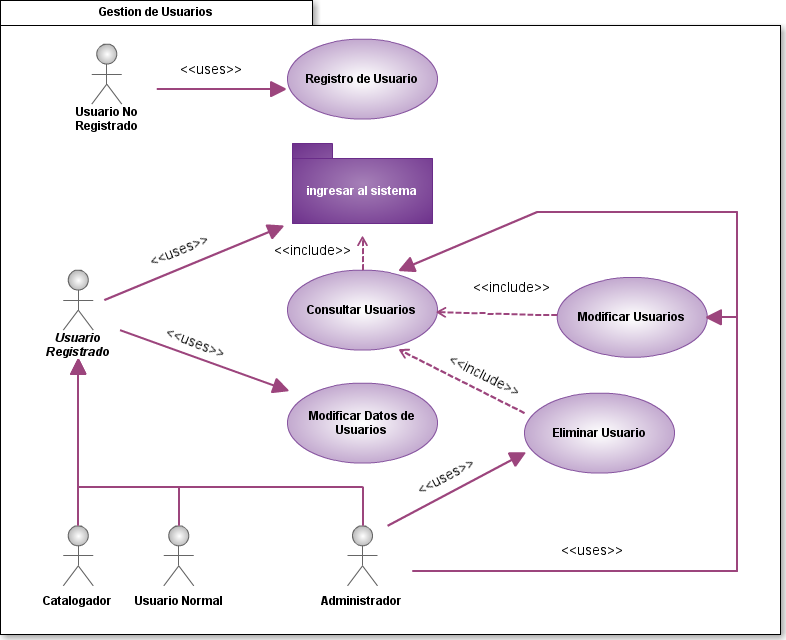
\includegraphics[scale=.6]{casosUso/CUGestionUsuarios}
        \end{minipage}     
        
        \begin{minipage}[c]{1\linewidth}
                \centering
                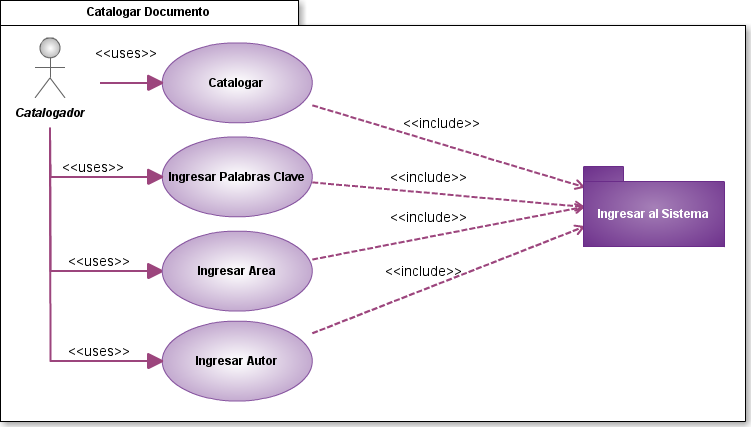
\includegraphics[width=16cm, height=14cm]{casosUso/CUCatalogar}
        \end{minipage}\\[5cm]
        
        \begin{minipage}[c]{1\linewidth}
                \centering
                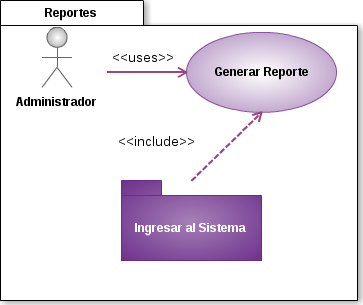
\includegraphics[scale=.7]{casosUso/CUReportes}
        \end{minipage}\\[2cm]
        
        \begin{minipage}[c]{1\linewidth}
                \begin{center}
                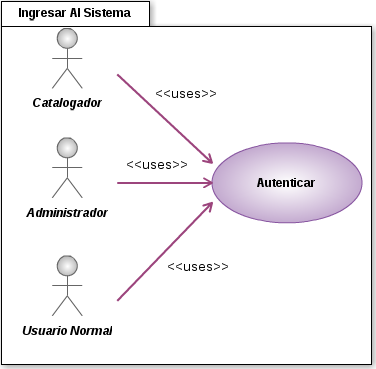
\includegraphics[scale=.7]{casosUso/CUAutenticar}                
                \end{center}
        \end{minipage}
        
        \begin{minipage}[c]{1\linewidth}
                \begin{center}
                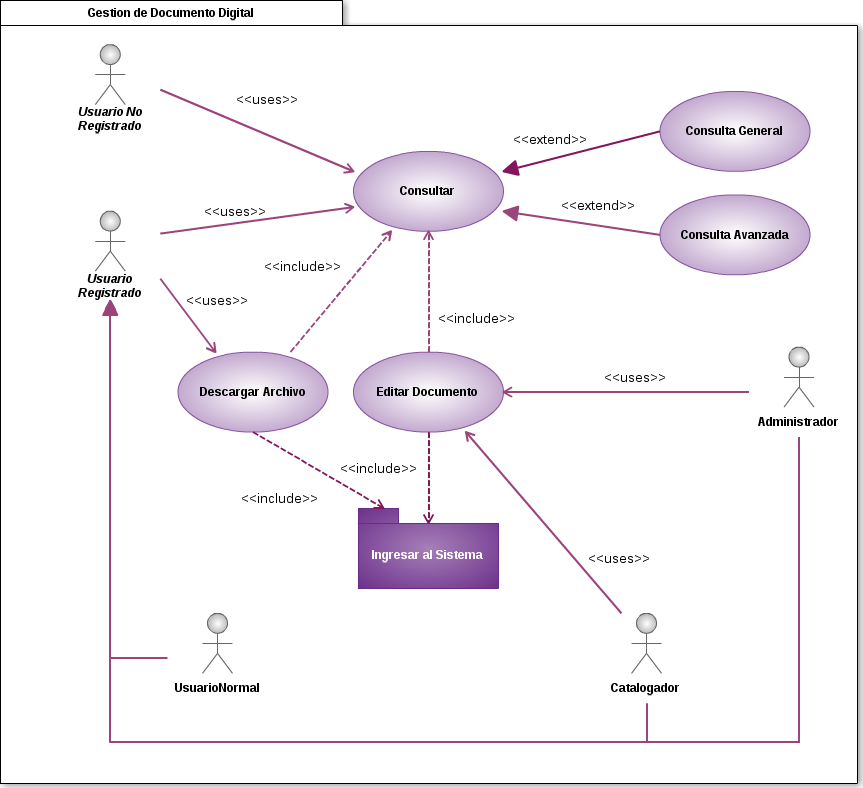
\includegraphics[scale=.5]{casosUso/CUGestionDocumento}
                \end{center}
        \end{minipage}
        
        
%---------------------------------------------------------------
        \newpage                
                \subsubsection{Especificación de casos de uso}
                        %\documentclass[]{article}
%\usepackage[spanish]{babel}
%\usepackage[utf8]{inputenc}
%\usepackage{geometry}
%\usepackage{colortbl}
%\usepackage{longtable}
%\usepackage{graphicx}
%\geometry{tmargin=3cm,bmargin=3cm,lmargin=3cm,rmargin=2cm}
%\begin{document}
\begin{center}
\begin{longtable}{|p{0.225\textwidth}|p{0.225\textwidth}|p{0.225\textwidth}|p{0.225\textwidth}|}
\hline
{\bf {Empresa:}} &
\multicolumn{2}{p{0.45\textwidth}|} { Escuela de Ingeniería de Sistemas y Computación } &
{
\includegraphics[width=80.5pt]{LOGO}} \\
\hline
\bf {Nombre del caso de uso:}&\multicolumn{3}{l|}{
Registro de Usuario.
} \\
\hline
\bf Código: & 
CU00 &\bf Fecha: & 
Abril 03 2011 \\
\hline
\bf Autor(es ): & 
Edgar Andrés Moncada & 
Yerminson Gonzalez & 
 \\
\hline
\bf Descripción: &\multicolumn{3}{p{0.675\textwidth}|}
{
Permite el registro al sistema de nuevos usuarios.
} \\
\hline
\bf Actores: &\multicolumn{3}{p{0.675\textwidth}|}{
Usuario No Registrado. 
} \\
\hline
\bf Precondiciones: &\multicolumn{3}{p{0.675\textwidth}|}
{
El sistema debe de haberse iniciado.
} \\
\hline
\multicolumn{4}{|c|}{\bf {Flujo Normal}}\\
\hline
\multicolumn{2}{|c}{\bf Actor} & \multicolumn{2}{|c|}{\bf Sistema } \\
\hline
\multicolumn{2}{|p{0.45\textwidth}}
{
\begin{itemize}
\item [1.]El caso de uso inicia cuando el usuario no registrado selecciona la opción de registrarse.
\item [3.] El usuario digita los campos pedidos.
\item[4.] El usuario le indica al sistema que valide los datos.
\end{itemize}
} &
\multicolumn{2}{|p{0.45\textwidth}|}
{
\begin{itemize}
\item[2.] El sistema genera una interfaz que le pide al usuario los siguientes datos obligatorios: login, contraseña, verificación de la contraseña, pregunta y respuesta secreta, nombre. A demás pide los siguientes datos que no son obligatorios: apellidos, género, fecha de nacimiento, email, nivel de escolaridad, vinculo con Univalle (estudiante de pregrado, de posgrado, egresado, profesor activo, jubilado, ninguno). Se pide información sobre las aéreas de interés.
\item[5.] El Sistema valida que el login no exista.
\item[6.] El Sistema valida que los campos de contraseña y verificación de contraseña.
 El sistema valida los campos digitados.
\item[7.] El sistema crea una nueva instancia del usuario en la base de datos.
\item[8.] El sistema envía un mensaje de confirmación al usuario y el caso de uso termina.
\end{itemize}
} \\
\hline
\multicolumn{4}{|c|}{\bf {Flujo Alternativo}}\\
\hline
\multicolumn{2}{|p{0.45\textwidth}}
{
\begin{itemize}
\item[3.3.] El Usuario no digita ninguno de los campos obligatorios.
\item[4.3.] El Usuario le indica al Sistema que valide los datos.
\end{itemize}
} &
\multicolumn{2}{|p{0.45\textwidth}|}
{
\begin{itemize}
\item[5.1.] El Sistema al validar se da cuenta que el login digitado por el Usuario ya existe.
\item[6.1. ]El Sistema envía una notificación al usuario indicándole que ingrese un nuevo login.
\item[6.2. ]El Sistema al validar se da cuenta que el campo de contraseña y el campo de verificación de contraseña no son iguales.
\item[7.2. ]El Sistema envía una notificación al Usuario indicándole que las contraseñas no coinciden y que las vuelva a confirmar.
\item[5.3. ]El Sistema al validar se da cuenta que los campos obligatorios no tienen datos.
\item[6.3.] El Sistema envía una notificación al Usuario indicándole que vuelva a confirmar.
\end{itemize}
} \\
\hline
\bf Poscondiciones: &\multicolumn{3}{p{0.675\textwidth}|}
{
El sistema almacena los datos del usuario en la base de datos.
} \\
\hline
\bf Excepciones: &\multicolumn{3}{p{0.675\textwidth}|}
{
El sistema no puede acceder a la base de datos y no puede almacenar los datos.
} \\
\hline
\bf Aprobado por : & 
 & \bf Fecha & 
 \\
\hline
\end{longtable}
\end{center}
%\end{document}
                        %%\pagebreak
                        
                        %\documentclass[]{article}
%\usepackage[spanish]{babel}
%\usepackage[utf8]{inputenc}
%\usepackage{geometry}
%\usepackage{colortbl}
%\usepackage{longtable}
%\usepackage{graphicx}
%\geometry{tmargin=3cm,bmargin=3cm,lmargin=3cm,rmargin=2cm}
%
%\begin{document}

\begin{center}
\begin{longtable}{|p{0.225\textwidth}|p{0.225\textwidth}|p{0.225\textwidth}|p{0.225\textwidth}|}
\hline
{\bf {Empresa:}} &
\multicolumn{2}{p{0.45\textwidth}|} { Escuela de Ingeniería de Sistemas y Computación } &
{
\includegraphics[width=80.5pt]{LOGO}} \\
\hline
\bf {Nombre del caso de uso:}&\multicolumn{3}{l|}{
Autenticar.
} \\
\hline
\bf Codigo: & 
CU01 &\bf Fecha: & 
Abril 02 2011 \\
\hline
\bf Autor(es ): & 
Edgar Andrés Moncada & 
 & 
 \\
\hline
\bf Descripcion: &\multicolumn{3}{p{0.675\textwidth}|}
{
Permite el ingreso y autenticación de los usuarios al sistema.
} \\
\hline
\bf Actores: &\multicolumn{3}{p{0.675\textwidth}|}{
Administrador, Catalogador, Usuario Normal. 
} \\
\hline
\bf Precondiciones: &\multicolumn{3}{p{0.675\textwidth}|}
{
Estar registrado en la biblioteca.
} \\
\hline
\multicolumn{4}{|c|}{\bf {Flujo Normal}}\\
\hline
\multicolumn{2}{|c}{\bf Actor} & \multicolumn{2}{|c|}{\bf Sistema } \\
\hline
\multicolumn{2}{|p{0.45\textwidth}}
{
\begin{itemize}
\item[1.] El Usuario selecciona la opción ingresar a la biblioteca.
\item[3.] El Usuario rellena los respectivos campos con su login y su contraseña y selecciona la opción ingresar.
\end{itemize}
} &
\multicolumn{2}{|p{0.45\textwidth}|}
{
\begin{itemize}
\item[2.] El sistema muestra los campos de login y contraseña.
\item[4.] El sistema verifica que el login exista y que la contraseña corresponde con la que se tiene almacenada.
\item[5.] El sistema actualiza el estado del usuario y el caso de uso termina.
\end{itemize}
} \\
\hline
\multicolumn{4}{|c|}{\bf {Flujo Alternativo}}\\
\hline
\multicolumn{2}{|p{0.45\textwidth}}
{} &
\multicolumn{2}{|p{0.45\textwidth}|}
{
\begin{itemize}
\item[4.1.]El Sistema alverificar se da cuenta que el login digitado por el usuario no existe
\item[5.1.]El Sistema indica que no existe el login y pide al usuario los datos de nuevo.
\item[4.2.] El Sistema al verificar se da cuenta que la contraseña digitada por el Usuario es errónea.
\item[5.2.] El Sistema envía una notificación indicando que la contraseña es errónea y que repita el proceso.
\end{itemize}
} \\
\hline
\bf Poscondiciones: &\multicolumn{3}{p{0.675\textwidth}|}
{
El sistema actualiza el perfil de usuario. El usuario identificado esta activo en el sistema.
} \\
\hline
\bf Excepciones: &\multicolumn{3}{p{0.675\textwidth}|}
{
El sistema no puede acceder a la base de datos y no puede verificar el login y/o la contraseña del usuario.
} \\
\hline
\bf Aprobado por : & 
 & \bf Fecha & 
 \\
\hline
\end{longtable}
\end{center}
%\end{document}
                        %%\pagebreak
                        
                        %\documentclass[]{article}
%\usepackage[spanish]{babel}
%\usepackage[utf8]{inputenc}
%\usepackage{geometry}
%\usepackage{colortbl}
%\usepackage{longtable}
%\usepackage{graphicx}
%\geometry{tmargin=3cm,bmargin=3cm,lmargin=3cm,rmargin=2cm}
%
%\begin{document}
\begin{center}
\begin{longtable}{|p{0.225\textwidth}|p{0.225\textwidth}|p{0.225\textwidth}|p{0.225\textwidth}|}
\hline
{\bf {Empresa:}} &
\multicolumn{2}{p{0.45\textwidth}|} { Escuela de Ingeniería de Sistemas y Computación } &
{
\includegraphics[width=80.5pt]{LOGO}} \\
\hline
\bf {Nombre del caso de uso:}&\multicolumn{3}{l|}{
Modificar usuarios.
} \\
\hline
\bf Codigo: & 
CU02 &\bf Fecha: & 
Abril 2 2011 \\
\hline
\bf Autor(es ): & 
Yerminson Gonzalez & 
Edgar Andrés Moncada & 
 \\
\hline
\bf Descripcion: &\multicolumn{3}{p{0.675\textwidth}|}
{
Permite la modificación de usuarios , es decir alguna de la información almacenada en el sistema.
} \\
\hline
\bf Actores: &\multicolumn{3}{p{0.675\textwidth}|}{
Administrador. 
} \\
\hline
\bf Precondiciones: &\multicolumn{3}{p{0.675\textwidth}|}
{
El administrador debe haber consultado sobre algún usuario.
} \\
\hline
\multicolumn{4}{|c|}{\bf {Flujo Normal}}\\
\hline
\multicolumn{2}{|c}{\bf Actor} & \multicolumn{2}{|c|}{\bf Sistema } \\
\hline
\multicolumn{2}{|p{0.45\textwidth}}
{
\begin{itemize}
\item[1. ]El caso de uso inicia cuando el administrador selecciona al usuario de la lista resultado.
\item[3.] El administrador modifica los datos de acuerdo a sus necesidades o ha una actualización de datos.
\end{itemize}
} &
\multicolumn{2}{|p{0.45\textwidth}|}
{
\begin{itemize}
\item[2.] El sistema responde a través de una interfaz que muestra los campos referente a sus atributos, donde se pueden modificar el estado o el perfil de algún usuario seleccionado el dato perfil de usuario puede ser: Usuario normal, Catalogador o administrador, el dato estado puede ser: Habilitado o deshabilitado.
\item[4. ]El sistema valida que todos los datos obligatorios se hayan suministrado.
\item[5. ]El sistema accede a la base de datos y realiza una verificación de los datos nuevos y existentes para que no hayan datos iguales donde no pueden serlo.
\item[6.] El sistema realiza la actualización de los datos en la base de datos con los datos suministrados según la preferencia del administrador.
\item[7.] El sistema responde a través de una interfaz de éxito donde muestra que se ha completado la operación y el caso de uso termina.
\end{itemize}
} \\
\hline
\multicolumn{4}{|c|}{\bf {Flujo Alternativo}}\\
\hline
\multicolumn{2}{|p{0.45\textwidth}}
{} &
\multicolumn{2}{|p{0.45\textwidth}|}
{
\begin{itemize}
\item[4.1.] El Sistema valida los datos y encuentra que hay errores.
\item[4.2.] El Sistema responde a través de una interfaz que muestra los campos referentes a los atributos para que sean llenados nuevamente, con información del error cometido.
\end{itemize}
} \\
\hline
\bf Poscondiciones: &\multicolumn{3}{p{0.675\textwidth}|}
{
Atributos de usuario en la base de datos modificados.
} \\
\hline
\bf Excepciones: &\multicolumn{3}{p{0.675\textwidth}|}
{
La base de datos puede desconectarse debido a fallos de energía.
} \\
\hline
\bf Aprobado por : & 
 & \bf Fecha & 
 \\
\hline
\end{longtable}
\end{center}
%\end{document}
                        %%\pagebreak
                        
                        %\documentclass[]{article}
%\usepackage[spanish]{babel}
%\usepackage[utf8]{inputenc}
%\usepackage{geometry}
%\usepackage{colortbl}
%\usepackage{longtable}
%\usepackage{graphicx}
%\geometry{tmargin=3cm,bmargin=3cm,lmargin=3cm,rmargin=2cm}
%
%\begin{document}
\begin{center}
\begin{longtable}{|p{0.225\textwidth}|p{0.225\textwidth}|p{0.225\textwidth}|p{0.225\textwidth}|}
\hline
{\bf {Empresa:}} &
\multicolumn{2}{p{0.45\textwidth}|} { Escuela de Ingeniería de Sistemas y Computación } &
{
\includegraphics[width=80.5pt]{LOGO}} \\
\hline
\bf {Nombre del caso de uso:}&\multicolumn{3}{l|}{
Modificar datos usuario.
} \\
\hline
\bf Codigo: & 
CU03 &\bf Fecha: & 
Abril 02 2011 \\
\hline
\bf Autor(es ): & 
Edgar Andrés Moncada & 
Yerminson Gonzalez & 
 \\
\hline
\bf Descripcion: &\multicolumn{3}{p{0.675\textwidth}|}
{
Permite la modificación de algunos datos del usuario.
} \\
\hline
\bf Actores: &\multicolumn{3}{p{0.675\textwidth}|}{
Usuario norma, Catalogador	y Administrador. 
} \\
\hline
\bf Precondiciones: &\multicolumn{3}{p{0.675\textwidth}|}
{
El usuario debe haberse logueado en el sistema.
} \\
\hline
\multicolumn{4}{|c|}{\bf {Flujo Normal}}\\
\hline
\multicolumn{2}{|c}{\bf Actor} & \multicolumn{2}{|c|}{\bf Sistema } \\
\hline
\multicolumn{2}{|p{0.45\textwidth}}
{
\begin{itemize}
\item[1. ]El caso de uso inicia cuando el usuario solicita editar su perfil.
\item[3. ]El usuario modifica los datos correspondientes de acuerdo a sus necesidades o ha una actualización de datos.
\end{itemize}
} &
\multicolumn{2}{|p{0.45\textwidth}|}
{
\begin{itemize}
\item[2. ]El sistema responde a través de una interfaz que muestra los campos referente a sus atributos, con los siguientes datos editables: contraseña, pregunta y respuesta secreta, nombre, apellidos, género, fecha nacimiento, nivel escolaridad, vinculo con univalle y áreas de interés. Los demás campos no son editables.
\item[4. ]El sistema valida de que los campos obligatorios contengan datos.
\item[5. ]El sistema accede a la base de datos y valida que los datos existentes y los nuevos datos no sean iguales cuando no pueden serlo.
\item[6. ]El sistema accede a la base de datos, y actualiza los valores de acuerdo a los suministrados por el usuario.
\item[7. ]El sistema responde a través de una interfaz de éxito donde muestra que se ha completado la operación.
 \end{itemize}
} \\
\hline
\multicolumn{4}{|c|}{\bf {Flujo Alternativo}}\\
\hline
\multicolumn{2}{|p{0.45\textwidth}}
{} &
\multicolumn{2}{|p{0.45\textwidth}|}
{
\begin{itemize}
\item[5.1.] El Sistema al validar los datos encuentra un error debido a que  el usuario lleno de manera incorrecta alguno de los campos correspondiente a la información editable  como: contraseña, pregunta y respuesta secreta, nombre, apellidos, género, fecha nacimiento, nivel escolaridad, vinculo con Univalle y áreas de interés.
\item[6.1.] El Sistema responde a través de una interfaz que muestra los campos referentes a los atributos para que sean llenados nuevamente, con información del error cometido.
\end{itemize} 
} \\
\hline
\bf Poscondiciones: &\multicolumn{3}{p{0.675\textwidth}|}
{
Atributos de usuario en la base de datos modificados.
} \\
\hline
\bf Excepciones: &\multicolumn{3}{p{0.675\textwidth}|}
{
La base de datos puede desconectarse debido a fallos de energía.
} \\
\hline
\bf Aprobado por : & 
 & \bf Fecha & 
 \\
\hline
\end{longtable}
\end{center}
%\end{document}
                        %%\pagebreak        
                        
                        %\documentclass[]{article}
%\usepackage[spanish]{babel}
%\usepackage[utf8]{inputenc}
%\usepackage{geometry}
%\usepackage{colortbl}
%\usepackage{longtable}
%\usepackage{graphicx}
%\geometry{tmargin=3cm,bmargin=3cm,lmargin=3cm,rmargin=2cm}
%
%\begin{document}
\begin{center}
\begin{longtable}{|p{0.225\textwidth}|p{0.225\textwidth}|p{0.225\textwidth}|p{0.225\textwidth}|}
\hline
{\bf {Empresa:}} &
\multicolumn{2}{p{0.45\textwidth}|} { Escuela de Ingeniería de Sistemas y Computación } &
{
\includegraphics[width=80.5pt]{LOGO}} \\
\hline
\bf {Nombre del caso de uso:}&\multicolumn{3}{l|}{
Ingresar tipos de material.
} \\
\hline
\bf Código: & 
CU07 &\bf Fecha: & 
Mayo 04 2011 \\
\hline
\bf Autor(es ): & 
Yerminson Gonzalez & 
 & 
 \\
\hline
\bf Descripción: &\multicolumn{3}{p{0.675\textwidth}|}
{
Permite la creación de nuevos tipos de material en caso de que se requiera para registro de un documento y que den información sobre la estructura del documento.
} \\
\hline
\bf Actores: &\multicolumn{3}{p{0.675\textwidth}|}{
Administrador y Catalogador. 
} \\
\hline
\bf Precondiciones: &\multicolumn{3}{p{0.675\textwidth}|}
{
Haber ingresado al sistema y tener perfil de catalogador o administrador.
} \\
\hline
\multicolumn{4}{|c|}{\bf {Flujo Normal}}\\
\hline
\multicolumn{2}{|c}{\bf Actor} & \multicolumn{2}{|c|}{\bf Sistema } \\
\hline
\multicolumn{2}{|p{0.45\textwidth}}
{
\begin{itemize}
\item[1. ]El caso de uso inicia cuando el catalogador solicita crear un tipo de material para algún documento.
\item[3.] El usuario ingresa datos en los campos proporcionado por la interfaz del sistema para creación de nuevos tipos de material.
\item[4. ]El usuario indica al sistema que ya a ingresado los datos y que desea crear el nuevo tipo de material.
\item[7. ]El usuario acepta el mensaje de confirmación generado por el sistema y el caso de uso finaliza.
\end{itemize}
} &
\multicolumn{2}{|p{0.45\textwidth}|}
{
\begin{itemize}
\item[2.] El sistema responde mostrando una interfaz con dos campos: un campo para indicar el nombre y un campo para indicar una descripción del tipo.
\item[5.] El sistema valida que el nombre del tipo de material que ha ingresado el usuario para el nuevo tipo de material no exista como nombre de otro tipo de material.
\item[6. ]El sistema crea un nuevo tipo de material para documentos de ciencias de la computación que serán almacenados en el sistema y responde con un mensaje al usuario indicando el éxito de la operación.
\end{itemize}
} \\
\hline
\multicolumn{4}{|c|}{\bf {Flujo Alternativo}}\\
\hline
\multicolumn{2}{|p{0.45\textwidth}}
{
\begin{itemize}
\item[7.1] El usuario acepta el mensaje de notificación del error generado por el sistema.
\end{itemize}
} &
\multicolumn{2}{|p{0.45\textwidth}|}
{
\begin{itemize}
\item[5.1] El sistema al realizar la validación del nombre se percata de que el nombre dado al nuevo tipo de material ya existe.
\item[6.1] El sistema genera un mensaje indicando que el nombre dado al tipo de material no se puede utilizar porque ya existe un tipo de material con ese nombre.
\end{itemize}
} \\
\hline
\bf Poscondiciones: &\multicolumn{3}{p{0.675\textwidth}|}
{
El sistema añade un registro correspondiente a los tipos de material a los que pueden pertenecer los documentos.
} \\
\hline
\bf Excepciones: &\multicolumn{3}{p{0.675\textwidth}|}
{
Fallo de conexionen la base de datos.	Falla en el sistema de suministro de energía.
} \\
\hline
\bf Aprobado por : & 
 & \bf Fecha & 
 \\
\hline
\end{longtable}
\end{center}
%\end{document}
                        %\pagebreak                                
                        
                        %\documentclass[]{article}
%\usepackage[spanish]{babel}
%\usepackage[utf8]{inputenc}
%\usepackage{geometry}
%\usepackage{colortbl}
%\usepackage{longtable}
%\usepackage{graphicx}
%\geometry{tmargin=3cm,bmargin=3cm,lmargin=3cm,rmargin=2cm}
%
%\begin{document}
\begin{center}
\begin{longtable}{|p{0.225\textwidth}|p{0.225\textwidth}|p{0.225\textwidth}|p{0.225\textwidth}|}
\hline
{\bf {Empresa:}} &
\multicolumn{2}{p{0.45\textwidth}|} { Escuela de Ingeniería de Sistemas y Computación } &
{
\includegraphics[width=80.5pt]{LOGO}} \\
\hline
\bf {Nombre del caso de uso:}&\multicolumn{3}{l|}{
Consultar usuarios.
} \\
\hline
\bf Código: & 
CU05 &\bf Fecha: & 
Abril 02 2011 \\
\hline
\bf Autor(es ): & 
Edgar Andrés Moncada & 
Yerminson Gonzalez & 
 \\
\hline
\bf Descripción: &\multicolumn{3}{p{0.675\textwidth}|}
{
Permite la consulta de usuarios que están registrados al sistema.
} \\
\hline
\bf Actores: &\multicolumn{3}{p{0.675\textwidth}|}{
Administrador. 
} \\
\hline
\bf Precondiciones: &\multicolumn{3}{p{0.675\textwidth}|}
{
El usuario debe haberse autentificado en el sistema y tener perfil de administrador.
} \\
\hline
\multicolumn{4}{|c|}{\bf {Flujo Normal}}\\
\hline
\multicolumn{2}{|c}{\bf Actor} & \multicolumn{2}{|c|}{\bf Sistema } \\
\hline
\multicolumn{2}{|p{0.45\textwidth}}
{
\begin{itemize}
\item[1. ]El caso de uso inicia cuando el cliente solicita la consulta de usuarios.
\item[3. ]El administrador escribe las palabras claves con respecto a la búsqueda y solicita al sistema que se realiza la búsqueda.
\end{itemize}
} &
\multicolumn{2}{|p{0.45\textwidth}|}
{
\begin{itemize}
 \item[2.] El sistema responde a través de una interfaz que permite introducir las palabras claves por las cuales se desea buscar algún usuario.
\item[4.] El sistema envía la consulta a la base de datos y con la información obtenida genera una interfaz donde muestra de manera organiza los resultados obtenidos.
\item[5.] El sistema envía esta interfaz al usuario como resultado de su consulta y el caso de uso termina.
\end{itemize}
} \\
\hline
\multicolumn{4}{|c|}{\bf {Flujo Alternativo}}\\
\hline
\multicolumn{2}{|p{0.45\textwidth}}
{} &
\multicolumn{2}{|p{0.45\textwidth}|}
{
\begin{itemize}
\item[4.1.] El Sistema realiza la consulta a la base de datos, y obtiene como resultado una consulta vacía debido  a que las palabras claves digitadas por el Usuario no coinciden con ninguno en la base datos..
\item[5.1.] EL sistema envía un mensaje informándole al Usuario de que no se encontraron coincidencias para esa búsqueda.
\end{itemize}
} \\
\hline
\bf Poscondiciones: &\multicolumn{3}{p{0.675\textwidth}|}
{
Se crea una vista temporal de los usuarios que han sido consultados.
} \\
\hline
\bf Excepciones: &\multicolumn{3}{p{0.675\textwidth}|}
{
a base de datos puede desconectarse debido a fallos de energía.
} \\
\hline
\bf Aprobado por : & 
 & \bf Fecha & 
 \\
\hline
\end{longtable}
\end{center}
%\end{document}
                        %\pagebreak
                        
                        %\documentclass[]{article}
%\usepackage[spanish]{babel}
%\usepackage[utf8]{inputenc}
%\usepackage{geometry}
%\usepackage{colortbl}
%\usepackage{longtable}
%\usepackage{graphicx}
%\geometry{tmargin=3cm,bmargin=3cm,lmargin=3cm,rmargin=2cm}
%
%\begin{document}
\begin{center}
\begin{longtable}{|p{0.225\textwidth}|p{0.225\textwidth}|p{0.225\textwidth}|p{0.225\textwidth}|}
\hline
{\bf {Empresa:}} &
\multicolumn{2}{p{0.45\textwidth}|} { Escuela de Ingeniería de Sistemas y Computación } &
{
\includegraphics[width=80.5pt]{LOGO}} \\
\hline
\bf {Nombre del caso de uso:}&\multicolumn{3}{l|}{
Catalogar.
} \\
\hline
\bf Código: & 
CU06 &\bf Fecha: & 
Abril 02 2011 \\
\hline
\bf Autor(es ): & 
Yerminson Gonzalez & 
 & 
 \\
\hline
\bf Descripción: &\multicolumn{3}{p{0.675\textwidth}|}
{
Permite la creación de un nuevo registro para un documento mediante su adecuada catalogacion es decir proporcionando los datos adecuados para su identificación y futura consulta.
} \\
\hline
\bf Actores: &\multicolumn{3}{p{0.675\textwidth}|}{
Catalogador. 
} \\
\hline
\bf Precondiciones: &\multicolumn{3}{p{0.675\textwidth}|}
{
Haber ingresado al sistema y tener perfil de catalogador.
} \\
\hline
\multicolumn{4}{|c|}{\bf {Flujo Normal}}\\
\hline
\multicolumn{2}{|c}{\bf Actor} & \multicolumn{2}{|c|}{\bf Sistema } \\
\hline
\multicolumn{2}{|p{0.45\textwidth}}
{
\begin{itemize}
\item[1.] El caso de uso inicia cuando el catalogador le solicita al sistema que permita catalogar un documento.
\item[3. ]El catalogador llena los campos correspondientes de acuerdo a la información que muestra el libro haciendo uso del listado que presenta algunos campos y otros que si se llenan mediante la especificación escrita del dato.  
\item[4. ]El catalogador solicita que sean verificados los datos al sistema al intentar guardar la información suministrada.
\item[7. ]El catalogador acepta el mensaje de éxito y así termina este caso de uso.
\end{itemize}
} &
\multicolumn{2}{|p{0.45\textwidth}|}
{
\begin{itemize}
\item[ 2.] El sistema le responde enviando una interfaz con los campos correspondientes a la información que se requiere para poder crear un nuevo registro de documento , los campos son: Tipo de material, número de identificación, título principal, título secundario y/o traducido, editorial, fecha publicación, fecha  catalogación, Fecha creación, Idioma, derechos de autor y una breve descripción o resumen del material.
\item[5.] El sistema valida los datos suministrados a través de la interfaz.
\item[6.] El sistema responde mostrando un mensaje de éxito que indica que la operación de registro del nuevo documento se llevo con éxito.
\end{itemize}
} \\
\hline
\multicolumn{4}{|c|}{\bf {Flujo Alternativo}}\\
\hline
\multicolumn{2}{|p{0.45\textwidth}}
{
\begin{itemize}
\item[4.2.] El Catalogador le indica al Sistema que desea suspender el registro del documento (para registrar una nueva área y/o autor).
\item[6.2.1.] El Catalogador le indica al Sistema que si desea salir.
\item[6.2.2.] El Catalogador le indica al Sistema que no desea salir y se continua el caso de uso en el flujo normal en 3.
\end{itemize}
} &
\multicolumn{2}{|p{0.45\textwidth}|}
{
\begin{itemize}
 \item[5.1.] El Sistema al validar los datos encuentra errores.
\item[6.1. ]El Sistema responde enviando un mensaje de error informando que alguno de los campos no se ha llenado de manera correcta y que debe ser corregido.
\item[5.2. ]El Sistema envía un mensaje de confirmación que indica si desea salir del proceso de registro.
\item[7.2.1.] El Sistema le informa que se ha cancelado el proceso y el caso de uso termina. 
\end{itemize}
} \\
\hline
\bf Poscondiciones: &\multicolumn{3}{p{0.675\textwidth}|}
{
El sistema añade un registro correspondiente a un nuevo documento.
} \\
\hline
\bf Excepciones: &\multicolumn{3}{p{0.675\textwidth}|}
{
Fallo de conexionen la base de datos. Falla en el sistema de suministro de energía.
} \\
\hline
\bf Aprobado por : & 
 & \bf Fecha & 
 \\
\hline
\end{longtable}
\end{center}
%\end{document}
                        %\pagebreak
                        
                        %\documentclass[]{article}
%\usepackage[spanish]{babel}
%\usepackage[utf8]{inputenc}
%\usepackage{geometry}
%\usepackage{colortbl}
%\usepackage{longtable}
%\usepackage{graphicx}
%\geometry{tmargin=3cm,bmargin=3cm,lmargin=3cm,rmargin=2cm}
%
%\begin{document}
\begin{center}
\begin{longtable}{|p{0.225\textwidth}|p{0.225\textwidth}|p{0.225\textwidth}|p{0.225\textwidth}|}
\hline
{\bf {Empresa:}} &
\multicolumn{2}{p{0.45\textwidth}|} { Escuela de Ingeniería de Sistemas y Computación } &
{
\includegraphics[width=80.5pt]{LOGO}} \\
\hline
\bf {Nombre del caso de uso:}&\multicolumn{3}{l|}{
Ingresar palabras clave.
} \\
\hline
\bf Codigo: & 
CU07 &\bf Fecha: & 
Abril 02 2011 \\
\hline
\bf Autor(es ): & 
Yerminson Gonzalez & 
 & 
 \\
\hline
\bf Descripcion: &\multicolumn{3}{p{0.675\textwidth}|}
{
Permite la creación de nuevas palabras claves en caso de que se requiera para registro de un documento y que den información sobre el tema que trata este documento.
} \\
\hline
\bf Actores: &\multicolumn{3}{p{0.675\textwidth}|}{
Administrador y Catalogador. 
} \\
\hline
\bf Precondiciones: &\multicolumn{3}{p{0.675\textwidth}|}
{
Haber ingresado al sistema y tener perfil de catalogador o administrador.
} \\
\hline
\multicolumn{4}{|c|}{\bf {Flujo Normal}}\\
\hline
\multicolumn{2}{|c}{\bf Actor} & \multicolumn{2}{|c|}{\bf Sistema } \\
\hline
\multicolumn{2}{|p{0.45\textwidth}}
{
\begin{itemize}
\item[1. ]El caso de uso inicia cuando el catalogador solicita crear una nueva palabra clave sobre un documento relacionado con las ciencias de la computación.
\item[3.] El catalogador ingresa datos en los campos proporcionado por la interfaz del sistema para creación de nuevas palabras claves.
\item[4. ]El catalogador indica al sistema que ya a ingresado los datos y que desea crear la nueva área.
\item[7. ]El acepta el mensaje de confirmación generado por el sistema y el caso de uso finaliza.
\end{itemize}
} &
\multicolumn{2}{|p{0.45\textwidth}|}
{
\begin{itemize}
\item[2.] El sistema responde mostrando una interfaz con dos campos: un campo para indicar el nombre y un campo para indicar una descripción del documento.
\item[5.] El sistema valida que el nombre de la palabra clave que ha ingresado el catalogador para la nueva palabra clave no exista como nombre de otra palabra clave.
\item[6. ]El sistema crea una nueva palabra clave con respecto a un documento de ciencias de la computación en el sistema y responde con un mensaje al usuario indicando el éxito de la operación.
\end{itemize}
} \\
\hline
\multicolumn{4}{|c|}{\bf {Flujo Alternativo}}\\
\hline
\multicolumn{2}{|p{0.45\textwidth}}
{
\begin{itemize}
\item[7.1] El usuario acepta el mensaje de notificación del error generado por el sistema.
\end{itemize}
} &
\multicolumn{2}{|p{0.45\textwidth}|}
{
\begin{itemize}
\item[5.1] El sistema al realizar la validación del nombre y se percata de que el nombre dado a la nueva palabra clave ya existe.
\item[6.1] El sistema genera un mensaje indicando que el nombre dado a la palabra clave no se puede utilizar porque ya existe un palabra clave con ese nombre.
\end{itemize}
} \\
\hline
\bf Poscondiciones: &\multicolumn{3}{p{0.675\textwidth}|}
{
El sistema añade un registro correspondiente a las palabras clave que pueden llevar los documentos.
} \\
\hline
\bf Excepciones: &\multicolumn{3}{p{0.675\textwidth}|}
{
Fallo de conexionen la base de datos.	Falla en el sistema de suministro de energía.
} \\
\hline
\bf Aprobado por : & 
 & \bf Fecha & 
 \\
\hline
\end{longtable}
\end{center}
%\end{document}
                        %\pagebreak        
                        
                        %\documentclass[10pt,a4paper]{article}
%
%
%\usepackage[spanish]{babel}
%\usepackage[utf8]{inputenc}
%\usepackage{geometry}
%\usepackage{colortbl}
%\usepackage{longtable}
%\usepackage{graphicx}
%
%\geometry{tmargin=1cm,bmargin=2cm,lmargin=2cm,rmargin=2cm}
%\begin{document}
\begin{center}


\begin{longtable}{|p{3cm}|p{3cm}|p{3cm}|p{3cm}|}

\hline
\bf {Empresa:} & \multicolumn{2}{|p{6cm}|}  { Escuela de Ingeniería de Sistemas y Computación }  & {
\includegraphics[width=80.5pt]{LOGO}} \\
\hline
\bf {Nombre del caso de uso:}&\multicolumn{3}{|p{6cm}|}{Ingresar Área} \\
\hline 
\bf Codigo: & CU08  &\bf Fecha: & \\

\hline 
\bf Autor(es ): & Yerminson Gonzalez    & Cristian Leonardo Ríos López & \\

\hline 
\bf Descripción: &\multicolumn{3}{|p{9cm}|}{ Permite la creación de nuevas áreas de ciencias de la computación en el Sistema} \\
\hline 
\bf Actores: &\multicolumn{3}{|p{9cm}|}{ Administrador, Catalogador } \\
\hline
\bf Precondiciones: &\multicolumn{3}{|p{9cm}|}{Tener el perfil de usuario Administrador o Catalogador.} \\
\hline
\multicolumn{4}{|c|}{\bf {Flujo Normal}}\\
\hline
\multicolumn{2}{|c|} {\bf Actor } & \multicolumn{2}{|c|}{\bf Sistema } \\
\hline
\multicolumn{2}{|p{6cm}|} {
\begin{itemize}
\item[1. ]El caso de uso inicia cuando el Usuario solicita crear una nueva área de ciencias de la computación.
\item[3.] El Usuario ingresa datos en los campos proporcionado por la interfaz del sistema para creación de nuevas áreas.
\item[4. ]El Usuario indica al Sistema que ya a ingresado los datos y que desea crear la nueva área.
\item[8. ] El Usuario acepta el mensaje de confirmación generado por el Sistema y el caso de uso finaliza.
\end{itemize}
} 
 & \multicolumn{2}{|p{6cm}|}{
 \begin{itemize}
\item[2.] El Sistema responde mostrando una interfaz con tres campos: un campo para indicar el nombre, un campo para indicar una descripción de la nueva área y un tercer campo donde se especifica la área a la que pertenece si la área que se esta ingresando es una subárea.
\item[5.]El Sistema valida que el nombre de la área que a ingresado el Usuario para la nueva área no exista como nombre de otra área.
\item[6. ]El Sistema valida que si lo que se esta creando es una subárea, el nombre que se haya indicado como área exista previamente en el Sistema.
\item[7.] El Sistema crea una nueva área de ciencias de la computación en el sistema y responde con un mensaje al Usuario indicando el éxito de la operación.
\end{itemize}
} \\
\hline
\multicolumn{4}{|c|}{\bf {Flujo Alternativo}}\\
\hline
\multicolumn{2}{|p{6cm}|} {
\begin{itemize}
\item[3.A.] El Usuario acepta el mensaje de notificación del error generado por el Sistema.
\item[3.B.] El Usuario acepta el mensaje de notificación del error generado por el Sistema
\end{itemize}} &
 \multicolumn{2}{|p{6cm}|}  {
 \begin{itemize}
\item[1.A.] El Sistema al realizar la validación del nombre y se percata de que el nombre dado a la nueva área ya existe.
\item[2.A.] El Sistema genera un mensaje indicando que el nombre dado al área no se puede utilizar porque ya existe un área con ese nombre.
\item[4. A.] El Sistema regresa a la interfaz que permite crear una nueva área de ciencias de la computación para que el Usuario indique otro nombre para continuar con la operación normalmente.
\item[1. B.] El Sistema al realizar la validación del nombre de la área cuando se esta creando una subárea se percata de que el nombre dado no existe en el Sistema como un área de ciencias de la computación.
\item[2. B. ]El Sistema genera un mensaje indicando que el nombre dado al área a la que pertenece la subárea no existe.
\item[4. B.] El Sistema regresa a la interfaz que permite crear una nueva área de ciencias de la computación para que el Usuario indique una nombre de área válido a la cual pertenece la subárea que se esta creando.
\end{itemize}}\\
\hline
\bf Poscondiciones: &\multicolumn{3}{|p{9cm}|}{El Sistema crea una nueva tupla de la base de datos correspondiente a la nueva área de ciencias de la computación.} \\
\hline
\bf Excepciones: &\multicolumn{3}{|p{9cm}|}{El Sistema no puede acceder a la base de datos y no puede crear la nueva tupla o realizar las consultas para las validaciones de los datos.} \\
\hline
\bf aprobado por : &   & \bf Fecha &  \\
\hline
\end{longtable}
\end{center}
%\end{document} 

                        %\pagebreak        
                        
                        %\documentclass[]{article}
%\usepackage[spanish]{babel}
%\usepackage[utf8]{inputenc}
%\usepackage{geometry}
%\usepackage{colortbl}
%\usepackage{longtable}
%\usepackage{graphicx}
%\geometry{tmargin=3cm,bmargin=3cm,lmargin=3cm,rmargin=2cm}
%
%\begin{document}
\begin{center}
\begin{longtable}{|p{0.225\textwidth}|p{0.225\textwidth}|p{0.225\textwidth}|p{0.225\textwidth}|}
\hline
{\bf {Empresa:}} &
\multicolumn{2}{p{0.45\textwidth}|} { Escuela de Ingeniería de Sistemas y Computación } &
{
\includegraphics[width=80.5pt]{LOGO}} \\
\hline
\bf {Nombre del caso de uso:}&\multicolumn{3}{l|}{
Ingresar Autor.
} \\
\hline
\bf Codigo: & 
CU09 &\bf Fecha: & 
Abril 02 2011 \\
\hline
\bf Autor(es ): & 
Yerminson Gonzalez & 
Cristian Ríos & 
 \\
\hline
\bf Descripcion: &\multicolumn{3}{p{0.675\textwidth}|}
{
Permite la creación de nuevos autores en el Sistema.
} \\
\hline
\bf Actores: &\multicolumn{3}{p{0.675\textwidth}|}{
Administrador, Catalogador. 
} \\
\hline
\bf Precondiciones: &\multicolumn{3}{p{0.675\textwidth}|}
{
Tener el perfil de usuario Administrador o catalogador.
} \\
\hline
\multicolumn{4}{|c|}{\bf {Flujo Normal}}\\
\hline
\multicolumn{2}{|c}{\bf Actor} & \multicolumn{2}{|c|}{\bf Sistema } \\
\hline
\multicolumn{2}{|p{0.45\textwidth}}
{
\begin{itemize}
\item[1. ]El caso de uso inicia cuando el Usuario solicita crear un nuevo autor
\item[3.] El Usuario ingresa datos en los campos proporcionado por la interfaz del sistema para creación de nuevos autores.
\item[4. ]El Usuario indica al Sistema que ya a ingresado los datos y que desea crear el nuevo autor.
\item[7.] El Usuario acepta el mensaje de confirmación generado por el sistema y el caso de uso finaliza.
\end{itemize}
} &
\multicolumn{2}{|p{0.45\textwidth}|}
{
\begin{itemize}
\item[2.]El Sistema responde mostrando una interfaz con cinco campos: identificación del autor, nombre, apellido, correo electrónico y el acrónimo.
\item[5.]El Sistema valida que la identificación del autor que a ingresado el usuario para el nuevo autor no exista como identificación de otro autor.
\item[6. ] El Sistema crea un nuevo autor en el sistema y responde con un mensaje al usuario indicando el éxito de la operación. 
\end{itemize}
} \\
\hline
\multicolumn{4}{|c|}{\bf {Flujo Alternativo}}\\
\hline
\multicolumn{2}{|p{0.45\textwidth}}
{
\begin{itemize}
\item[7.1.] El Usuario acepta el mensaje de notificación del error generado por el sistema.
\end{itemize}
} &
\multicolumn{2}{|p{0.45\textwidth}|}
{
\begin{itemize}
\item[5.1.] El sistema valida  los datos y encuenta un error en los campos que han sido diligenciados por el Usuario tales como: nombre, apellido, correo electrónico y el acrónimo.
\item[6.1.] El sistema envía un mensaje notificando del error a la hora de llenar los campos.
\end{itemize}
} \\
\hline
\bf Poscondiciones: &\multicolumn{3}{p{0.675\textwidth}|}
{
El Sistema crea una nueva tupla de la base de datos correspondiente a la nueva área de ciencias de la computación.
} \\
\hline
\bf Excepciones: &\multicolumn{3}{p{0.675\textwidth}|}
{
El Sistema no puede acceder a la base de datos y no puede crear la nueva tupla o realizar las consultas para las validaciones de los datos.
} \\
\hline
\bf Aprobado por : & 
 & \bf Fecha & 
 \\
\hline
\end{longtable}
\end{center}
%\end{document}
                        %\pagebreak                        
                        
                        %\documentclass[]{article}
%\usepackage[spanish]{babel}
%\usepackage[utf8]{inputenc}
%\usepackage{geometry}
%\usepackage{colortbl}
%\usepackage{longtable}
%\usepackage{graphicx}
%\geometry{tmargin=3cm,bmargin=3cm,lmargin=3cm,rmargin=2cm}
%
%\begin{document}
\begin{center}
\begin{longtable}{|p{0.225\textwidth}|p{0.225\textwidth}|p{0.225\textwidth}|p{0.225\textwidth}|}
\hline
{\bf {Empresa:}} &
\multicolumn{2}{p{0.45\textwidth}|} { Escuela de Ingeniería de Sistemas y Computación } &
{
\includegraphics[width=80.5pt]{LOGO}} \\
\hline
\bf {Nombre del caso de uso:}&\multicolumn{3}{l|}{
Generar Reporte Documento
} \\
\hline
\bf Codigo: & 
CU10 &\bf Fecha: & 
Abril 03 2011 \\
\hline
\bf Autor(es ): & 
Edgar Andrés Moncada & 
 & 
 \\
\hline
\bf Descripcion: &\multicolumn{3}{p{0.675\textwidth}|}
{
Permite la generación de reportes que tengan que ver con los Usuarios del Sistema.
} \\
\hline
\bf Actores: &\multicolumn{3}{p{0.675\textwidth}|}{
Administrador 
} \\
\hline
\bf Precondiciones: &\multicolumn{3}{p{0.675\textwidth}|}
{
El Administrador debe estar haberse autenticado en el sistema.
} \\
\hline
\multicolumn{4}{|c|}{\bf {Flujo Normal}}\\
\hline
\multicolumn{2}{|c}{\bf Actor} & \multicolumn{2}{|c|}{\bf Sistema } \\
\hline
\multicolumn{2}{|p{0.45\textwidth}}
{
\begin{itemize}
\item[1. ]El caso de uso inicia cuando el Administrador selecciona la opción Generar Reportes de Usuarios.
\item[3.]El Administrador ingresa los datos en los campos y selecciona las opciones para el reporte.
\item[4. ]El Administrador selecciona la opción Generar Reporte.
\item[6.] El Administrador selecciona el lugar y le da el nombre a reporte.
\item[7.] El Administrador selecciona la opción guardar.
\end{itemize}
} &
\multicolumn{2}{|p{0.45\textwidth}|}
{
\begin{itemize}
\item[2.]El Sistema muestra los campos y las diferentes opciones para generar reportes de los usuarios.
\item[5.]El Sistema muestra una interfaz para elegir el lugar donde se almacenara el documento y el nombre que se le colocara.
\item[8. ]El Sistema envía una notificación de que se genero el reporte y el caso de uso termina.
\end{itemize}
} \\
\hline
\multicolumn{4}{|c|}{\bf {Flujo Alternativo}}\\
\hline
\multicolumn{2}{|p{0.45\textwidth}}
{
\begin{itemize}
\item[4.1.] El Administrador decide no generar ningún reporte y selecciona opción y el caso de uso termina.
\item[6.2.] El Administrador no selecciona ningún lugar o  no le da ningún nombre para guardar el documento.
\end{itemize}
} &
\multicolumn{2}{|p{0.45\textwidth}|}
{
\begin{itemize}
 \item[7.2] El Sistema envia un mensaje indicando que el reporte no fue generado y el caso de uso termina.
 \end{itemize}
} \\
\hline
\bf Poscondiciones: &\multicolumn{3}{p{0.675\textwidth}|}
{
Se genera un reporte en formato pdf.
} \\
\hline
\bf Excepciones: &\multicolumn{3}{p{0.675\textwidth}|}
{
No se pude acceder a la base de datos para obtener los datos seleccionados por el Administrador.
} \\
\hline
\bf Aprobado por : & 
 & \bf Fecha & 
 \\
\hline
\end{longtable}
\end{center}
%\end{document}
                        %\pagebreak
                        
                        %\documentclass[]{article}
%\usepackage[spanish]{babel}
%\usepackage[utf8]{inputenc}
%\usepackage{geometry}
%\usepackage{colortbl}
%\usepackage{longtable}
%\usepackage{graphicx}
%\geometry{tmargin=3cm,bmargin=3cm,lmargin=3cm,rmargin=2cm}
%
%\begin{document}
\begin{center}
\begin{longtable}{|p{0.225\textwidth}|p{0.225\textwidth}|p{0.225\textwidth}|p{0.225\textwidth}|}
\hline
{\bf {Empresa:}} &
\multicolumn{2}{p{0.45\textwidth}|} { Escuela de Ingeniería de Sistemas y Computación } &
{
\includegraphics[width=80.5pt]{LOGO}} \\
\hline
\bf {Nombre del caso de uso:}&\multicolumn{3}{l|}{
Consulta General.
} \\
\hline
\bf Código: & 
CU11 &\bf Fecha: & 
Abril 02 2011 \\
\hline
\bf Autor(es ): & 
Edgar Andrés Moncada  & 
 & 
 \\
\hline
\bf Descripción: &\multicolumn{3}{p{0.675\textwidth}|}
{
Permite la realización de consulta de los documentos digitales del Sistema de manera General.
} \\
\hline
\bf Actores: &\multicolumn{3}{p{0.675\textwidth}|}{
Administrador, Catalogador, Usuario Normal, Usuario No Registrado 
} \\
\hline
\bf Precondiciones: &\multicolumn{3}{p{0.675\textwidth}|}
{
El Sistema se haya iniciado.
} \\
\hline
\multicolumn{4}{|c|}{\bf {Flujo Normal}}\\
\hline
\multicolumn{2}{|c}{\bf Actor} & \multicolumn{2}{|c|}{\bf Sistema } \\
\hline
\multicolumn{2}{|p{0.45\textwidth}}
{
\begin{itemize}
\item[1. ]El caso de uso inicia cuando el Usuario va a realizar una consulta.
\item[3.]El Usuario ingresa datos en el campo de texto y selecciona la opción consultar.
\item[6. ]El Usuario selecciona uno de los resultados de la consulta. 
\end{itemize}
} &
\multicolumn{2}{|p{0.45\textwidth}|}
{
\begin{itemize}
\item[2.]El Sistema muestra un campo de texto para el ingreso de datos por parte del usuario.
\item[4.]El Sistema realiza la consulta
\item[5. ]El Sistema muestra un listado de los resultados de la consulta.
\item[7. ] El Sistema muestra todos los datos relacionados con el documento y el caso de uso termina.
\end{itemize}
} \\
\hline
\multicolumn{4}{|c|}{\bf {Flujo Alternativo}}\\
\hline
\multicolumn{2}{|p{0.45\textwidth}}
{
\begin{itemize}
\item[6.1.] El Usuario no selecciona ninguno de los resultados de la consulta y el caso de uso termina.
\end{itemize}
} &
\multicolumn{2}{|p{0.45\textwidth}|}
{
\begin{itemize}
\item[4.1.]  El Sistema realiza la consulta y esta no tiene resultados debido a que el usuario dígito en el campo algunas palabras que no coincidían para una consulta valida.
\item[5.1] El Sistema envía una notificación indicando que no se encontraron coincidencias.
 \end{itemize}
} \\
\hline
\bf Poscondiciones: &\multicolumn{3}{p{0.675\textwidth}|}
{
Se muestra las consultas relacionadas con los datos que ingreso el Usuario.
} \\
\hline
\bf Excepciones: &\multicolumn{3}{p{0.675\textwidth}|}
{
No se pude acceder a la base de datos para obtener los datos de los Documentos Digitales.
} \\
\hline
\bf Aprobado por : & 
 & \bf Fecha & 
 \\
\hline
\end{longtable}
\end{center}
%\end{document}
                        %\pagebreak
                        
                        %\documentclass[]{article}
%\usepackage[spanish]{babel}
%\usepackage[utf8]{inputenc}
%\usepackage{geometry}
%\usepackage{colortbl}
%\usepackage{longtable}
%\usepackage{graphicx}
%\geometry{tmargin=3cm,bmargin=3cm,lmargin=3cm,rmargin=2cm}
%
%\begin{document}
\begin{center}
\begin{longtable}{|p{0.225\textwidth}|p{0.225\textwidth}|p{0.225\textwidth}|p{0.225\textwidth}|}
\hline
{\bf {Empresa:}} &
\multicolumn{2}{p{0.45\textwidth}|} { Escuela de Ingeniería de Sistemas y Computación } &
{
\includegraphics[width=80.5pt]{LOGO}} \\
\hline
\bf {Nombre del caso de uso:}&\multicolumn{3}{l|}{
Consulta Avanzada.
} \\
\hline
\bf Codigo: & 
CU12 &\bf Fecha: & 
Abril 02 2011 \\
\hline
\bf Autor(es ): & 
Edgar Andrés Moncada & 
 & 
 \\
\hline
\bf Descripcion: &\multicolumn{3}{p{0.675\textwidth}|}
{
Permite la realización de consulta de los documentos digitales del Sistema de manera Avanzada.
} \\
\hline
\bf Actores: &\multicolumn{3}{p{0.675\textwidth}|}{
Administrador, Catalogador, Usuario Normal, Usuario No Registrado 
} \\
\hline
\bf Precondiciones: &\multicolumn{3}{p{0.675\textwidth}|}
{
El Sistema se haya iniciado.
} \\
\hline
\multicolumn{4}{|c|}{\bf {Flujo Normal}}\\
\hline
\multicolumn{2}{|c}{\bf Actor} & \multicolumn{2}{|c|}{\bf Sistema } \\
\hline
\multicolumn{2}{|p{0.45\textwidth}}
{
\begin{itemize}
\item[1. ]El caso de uso inicia cuando el Usuario va a realizar una consulta y selecciona la opción de Consulta Avanzada.
\item[3.]El Usuario ingresa datos en alguno o en combinaciones de los campos de texto, seleccionando los parámetros deseados y selecciona la opción consultar.
\item[6. ]El Usuario selecciona uno de los resultados de la consulta. 
\end{itemize}
} &
\multicolumn{2}{|p{0.45\textwidth}|}
{
\begin{itemize}
\item[2.]El Sistema muestra una interface 3 campos de texto para Titulo, Autor y Palabra Clave con la posibilidad de seleccionar para cada una las restricciones de con todas las palabras, con algunas de las palabras o con ninguna de las palabras; Incluye también los parámetros de Área, Idioma, Fecha de Publicación y Formato del Archivo.
\item[4. ]El Sistema realiza la consulta.
\item[5. ]El Sistema muestra un listado de los resultados de la consulta.
\item[7. ] El Sistema muestra todos los datos relacionados con el documento y el caso de uso termina.
\end{itemize}
} \\
\hline
\multicolumn{4}{|c|}{\bf {Flujo Alternativo}}\\
\hline
\multicolumn{2}{|p{0.45\textwidth}}
{
\begin{itemize}
 \item[6.2. ] El Usuario no selecciona ninguno de los resultados de la consulta y el caso de uso termina.
\end{itemize}
} &
\multicolumn{2}{|p{0.45\textwidth}|}
{
\begin{itemize}
 \item[5.1. ] La consulta no arroja ningun resultado.
 \item[6.1. ] El Sistema envía una notificación indicando que no se encontraron coincidencias.
 \end{itemize}
} \\
\hline
\bf Poscondiciones: &\multicolumn{3}{p{0.675\textwidth}|}
{
Se muestra las consultas relacionadas con los datos que ingreso el Usuario.
} \\
\hline
\bf Excepciones: &\multicolumn{3}{p{0.675\textwidth}|}
{
No se pude acceder a la base de datos para obtener los datos de los Documentos Digitales.
} \\
\hline
\bf Aprobado por : & 
 & \bf Fecha & 
 \\
\hline
\end{longtable}
\end{center}
%\end{document}
                        %\pagebreak
                        
                        %\documentclass[]{article}
%\usepackage[spanish]{babel}
%\usepackage[utf8]{inputenc}
%\usepackage{geometry}
%\usepackage{colortbl}
%\usepackage{longtable}
%\usepackage{graphicx}
%\geometry{tmargin=3cm,bmargin=3cm,lmargin=3cm,rmargin=2cm}
%
%\begin{document}
\begin{center}
\begin{longtable}{|p{0.225\textwidth}|p{0.225\textwidth}|p{0.225\textwidth}|p{0.225\textwidth}|}
\hline
{\bf {Empresa:}} &
\multicolumn{2}{p{0.45\textwidth}|} { Escuela de Ingeniería de Sistemas y Computación } &
{
\includegraphics[width=80.5pt]{LOGO}} \\
\hline
\bf {Nombre del caso de uso:}&\multicolumn{3}{l|}{
Descargar Archivo.
} \\
\hline
\bf Codigo: & 
CU13 &\bf Fecha: & 
Abril 02 2011 \\
\hline
\bf Autor(es ): & 
Edgar Andrés Moncada & 
 & 
 \\
\hline
\bf Descripcion: &\multicolumn{3}{p{0.675\textwidth}|}
{
Permite a un Usuario Registrado Descargar los diferentes Documentos Digitales almacenados en el Sistema.
} \\
\hline
\bf Actores: &\multicolumn{3}{p{0.675\textwidth}|}{
Usuario Normal, Catalogador, Administrador. 
} \\
\hline
\bf Precondiciones: &\multicolumn{3}{p{0.675\textwidth}|}
{
El Sistema se haya iniciado.Haber realizado una consulta del Documento y seleccionado un resultado.
} \\
\hline
\multicolumn{4}{|c|}{\bf {Flujo Normal}}\\
\hline
\multicolumn{2}{|c}{\bf Actor} & \multicolumn{2}{|c|}{\bf Sistema } \\
\hline
\multicolumn{2}{|p{0.45\textwidth}}
{
\begin{itemize}
\item[1. ]. El Usuario Registrado inicia el caso de uso al seleccionar la opción Descargar.
\item[3.]El Usuario Registrado ingresa el nombre y selecciona el lugar donde almacenará el documento.
\end{itemize}
} &
\multicolumn{2}{|p{0.45\textwidth}|}
{
\begin{itemize}
\item[2.]El Sistema muestra una interfaz para seleccionar el nombre y el lugar donde se almacenara el documento.
\item[4.]El Sistema almacena el archivo.
\item[5. ]. El Sistema muestra una notificación de que se realizo el procedimiento correctamente y el caso de uso termina.
\end{itemize}
} \\
\hline
\multicolumn{4}{|c|}{\bf {Flujo Alternativo}}\\
\hline
\multicolumn{2}{|p{0.45\textwidth}}
{
\begin{itemize}
\item[3.1.] El Usuario no elige ningún lugar para almacenar el Documento y el caso de uso termina.
\end{itemize}
} &
\multicolumn{2}{|p{0.45\textwidth}|}
{ } \\
\hline
\bf Poscondiciones: &\multicolumn{3}{p{0.675\textwidth}|}
{
El Sistema almacena la fecha, el tipo de usuario y el documento que fue descargado. Se almacena el Documento Digital en el formato en que se encuentra almacenado.
} \\
\hline
\bf Excepciones: &\multicolumn{3}{p{0.675\textwidth}|}
{
No se puede acceder al repositorio donde estan almacenado los Docuemntos Digitales del Sistema.
} \\
\hline
\bf Aprobado por : & 
 & \bf Fecha & 
 \\
\hline
\end{longtable}
\end{center}
%\end{document}
                        %\pagebreak
                        %\documentclass[]{article}
%\usepackage[spanish]{babel}
%\usepackage[utf8]{inputenc}
%\usepackage{geometry}
%\usepackage{colortbl}
%\usepackage{longtable}
%\usepackage{graphicx}
%\geometry{tmargin=3cm,bmargin=3cm,lmargin=3cm,rmargin=2cm}
%
%\begin{document}
\begin{center}
\begin{longtable}{|p{0.225\textwidth}|p{0.225\textwidth}|p{0.225\textwidth}|p{0.225\textwidth}|}
\hline
{\bf {Empresa:}} &
\multicolumn{2}{p{0.45\textwidth}|} { Escuela de Ingeniería de Sistemas y Computación } &
{
\includegraphics[width=80.5pt]{LOGO}} \\
\hline
\bf {Nombre del caso de uso:}&\multicolumn{3}{l|}{
Editar información del Documento.
} \\
\hline
\bf Código: & 
CU14 &\bf Fecha: & 
Abril 02 2011 \\
\hline
\bf Autor(es ): & 
Edgar Andrés Moncada & 
 & 
 \\
\hline
\bf Descripción: &\multicolumn{3}{p{0.675\textwidth}|}
{
Permite modificar los metadatos de los Documentos Digitales del Sistema.
} \\
\hline
\bf Actores: &\multicolumn{3}{p{0.675\textwidth}|}{
Catalogador, Administrador. 
} \\
\hline
\bf Precondiciones: &\multicolumn{3}{p{0.675\textwidth}|}
{
Haber realizado una consulta del Documento y seleccionado uno de los resultados.
} \\
\hline
\multicolumn{4}{|c|}{\bf {Flujo Normal}}\\
\hline
\multicolumn{2}{|c}{\bf Actor} & \multicolumn{2}{|c|}{\bf Sistema } \\
\hline
\multicolumn{2}{|p{0.45\textwidth}}
{
\begin{itemize}
\item[1. ] El caso de uso inicia cuando el Usuario a seleccionado la opción de Editar Documento.
\item[3.]El Usuario rellena los campos y selecciona los parámetros del Documento, y selecciona la opción Actualizar.
\end{itemize}
} &
\multicolumn{2}{|p{0.45\textwidth}|}
{
\begin{itemize}
\item[2.]El Sistema muestra una interface con los campos y los parámetros para modificar los metadatos del Documento Digital: Tipo de material, número de identificación, título principal, título secundario y/o traducido, editorial, fecha publicación, fecha  catalogación, Fecha creación, Idioma, derechos de autor y una breve descripción o resumen del material.
\item[4.]El Sistema valida los datos.
\item[5. ] El Sistema actualiza los datos almacenados del Documento Digital.
\item[6. ]El Sistema muestra una notificación de que se realizo con éxito la actualización y termina el caso de uso.
\end{itemize}
} \\
\hline
\multicolumn{4}{|c|}{\bf {Flujo Alternativo}}\\
\hline
\multicolumn{2}{|p{0.45\textwidth}}
{ } &
\multicolumn{2}{|p{0.45\textwidth}|}
{
\begin{itemize}
\item[4.1.] El Sistema valida los datos y se da cuenta que hay datos erróneos.
\item[5.1.] El Sistema envía una notificación de cuales son los campos con datos erróneos.
\end{itemize} 
} \\
\hline
\bf Poscondiciones: &\multicolumn{3}{p{0.675\textwidth}|}
{
El Sistema almacena la fecha, el tipo de usuario y el documento que fue descargado. Se almacena el Documento Digital en el formato en que se encuentra almacenado.
} \\
\hline
\bf Excepciones: &\multicolumn{3}{p{0.675\textwidth}|}
{
No se puede acceder al repositorio donde están almacenado los Documentos Digitales del Sistema.
} \\
\hline
\bf Aprobado por : & 
 & \bf Fecha & 
 \\
\hline
\end{longtable}
\end{center}
%\end{document}
                        %\pagebreak                        
 
\section{Análisis}
		\subsection{Diagrama de Clases}
			\begin{minipage}[c]{1\linewidth}
				\centering
				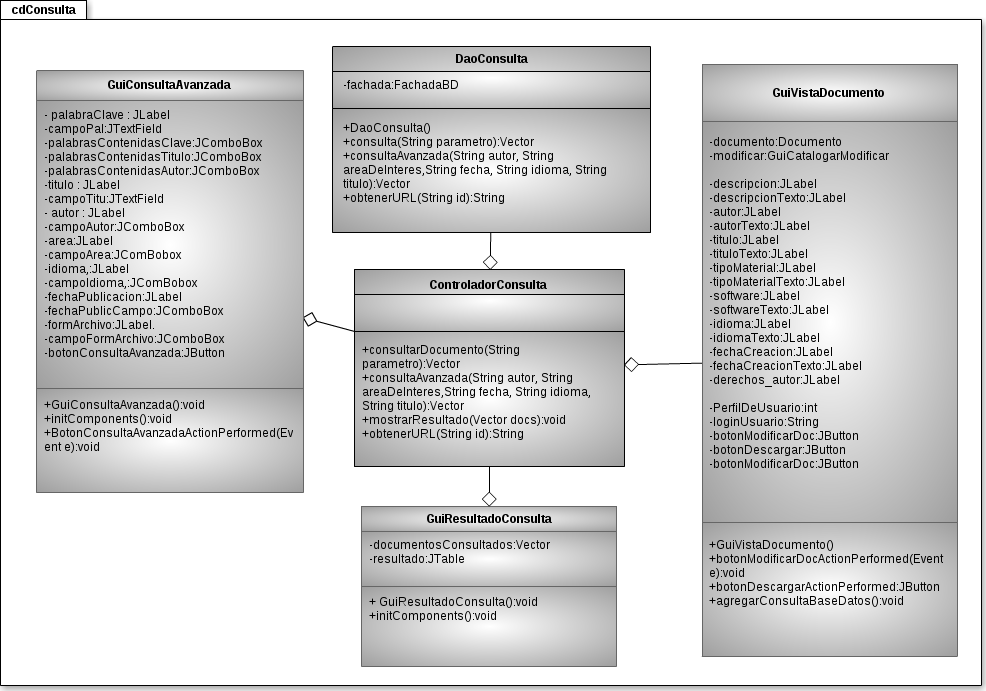
\includegraphics[width=17cm, height=14cm]{DiagramasClase/Consultas}
			\end{minipage}	
		
			\begin{minipage}[c]{1\linewidth}
				\centering
				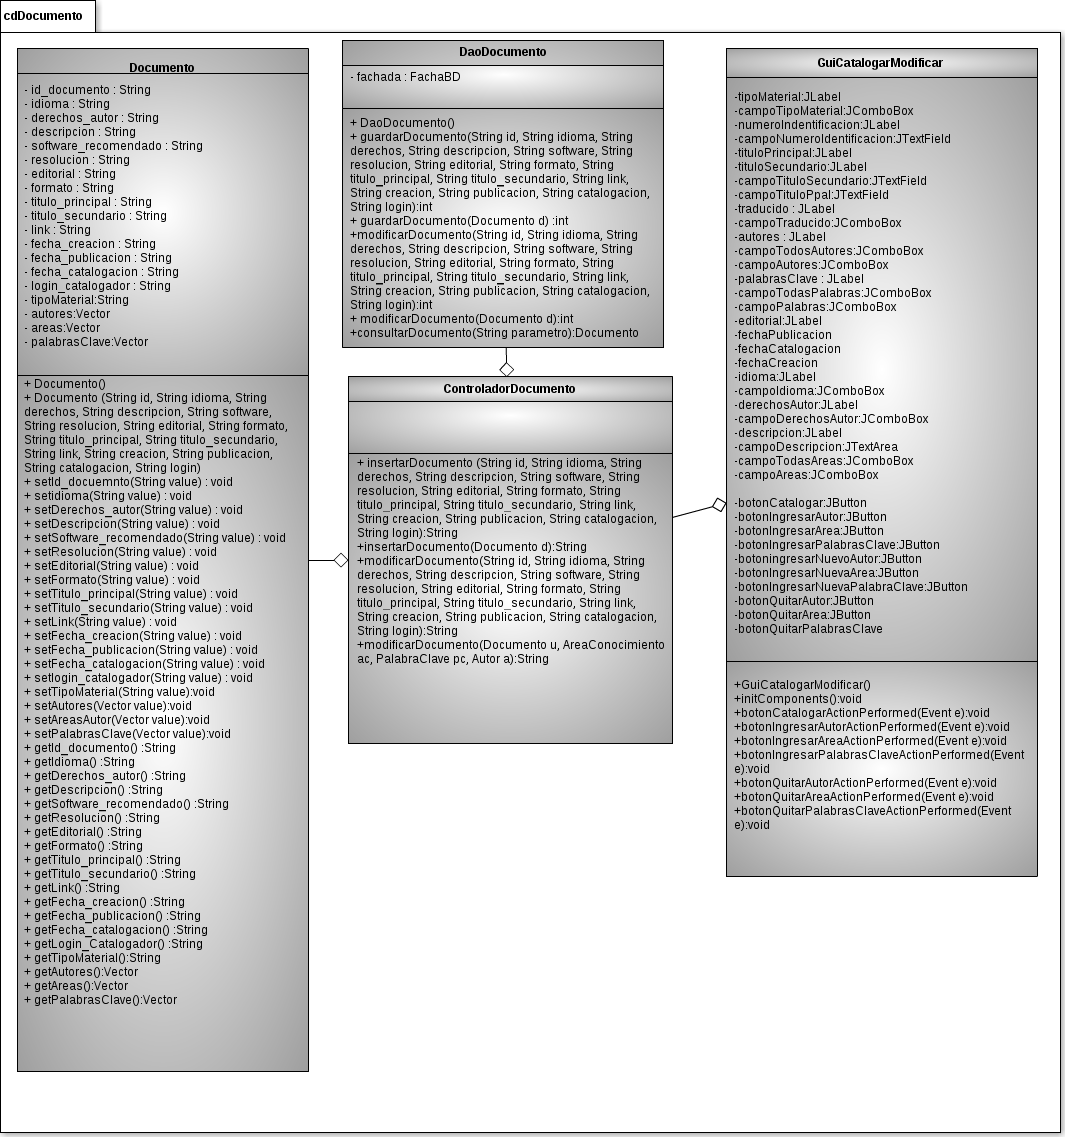
\includegraphics[width=17cm, height=20cm]{DiagramasClase/Documentos}
			\end{minipage}	
		
			\begin{minipage}[c]{1\linewidth}
				\centering
				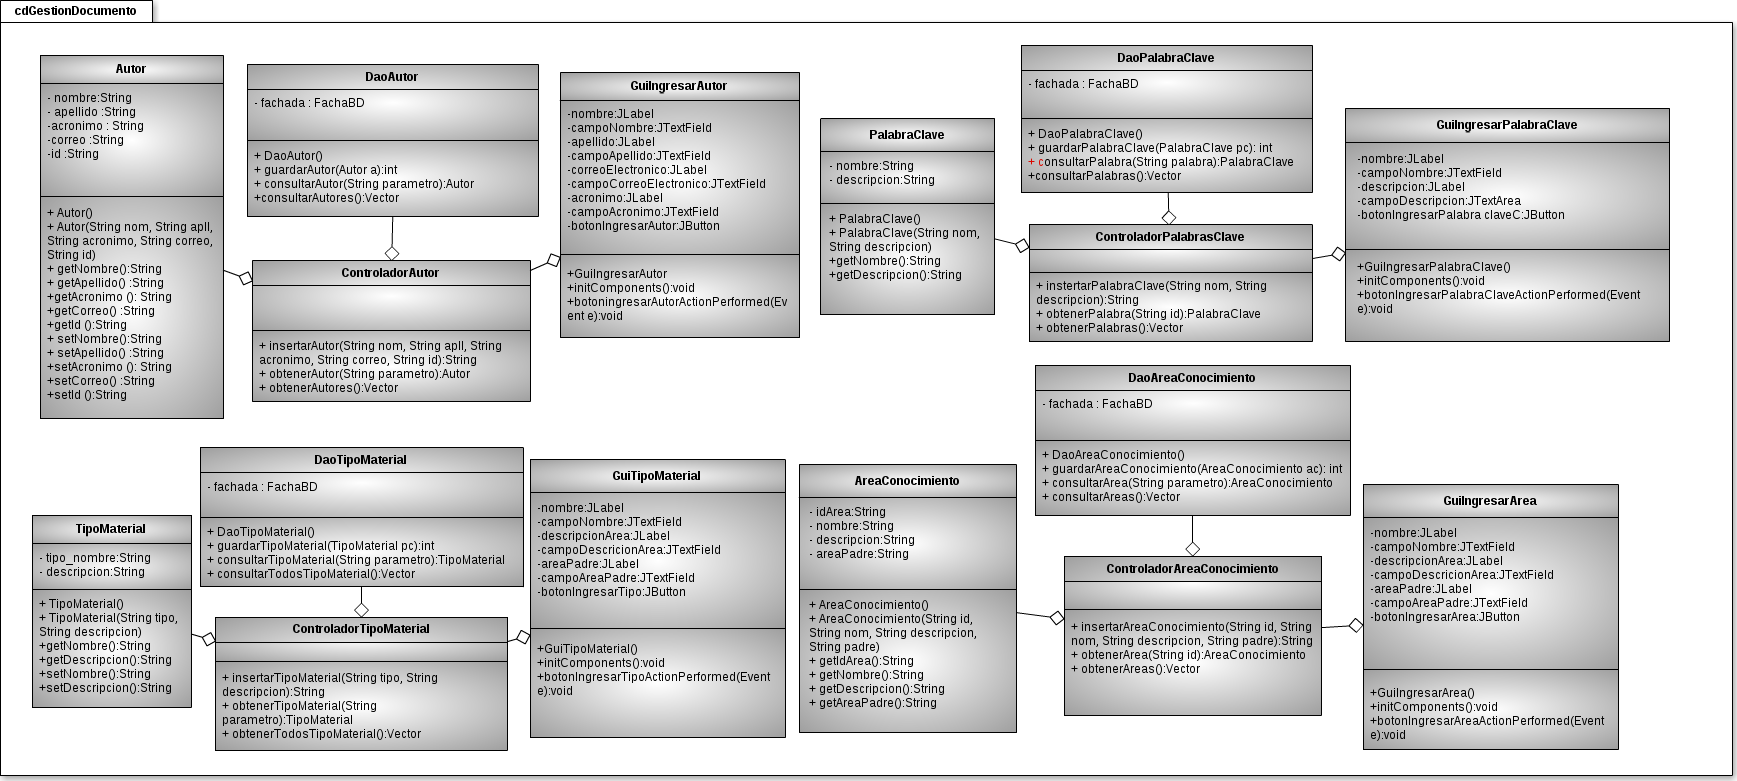
\includegraphics[width=22cm, height=17cm,angle=90]{DiagramasClase/GestionDocumento}
			\end{minipage}	
		
			\begin{minipage}[c]{1\linewidth}
				\centering
				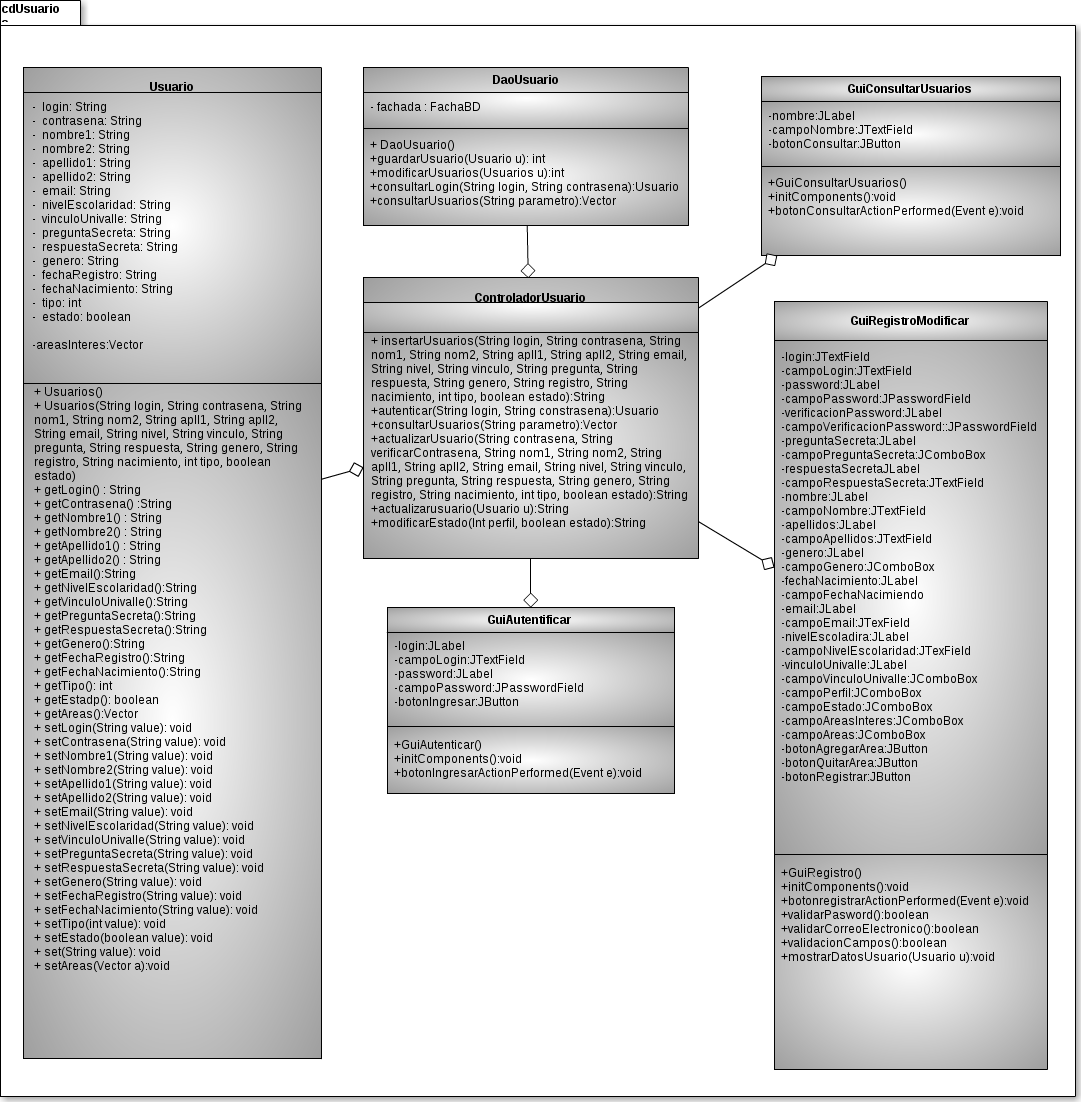
\includegraphics[width=17cm, height=22cm]{DiagramasClase/Usuarios}
			\end{minipage}	
		
			\begin{minipage}[c]{1\linewidth}
				\centering
				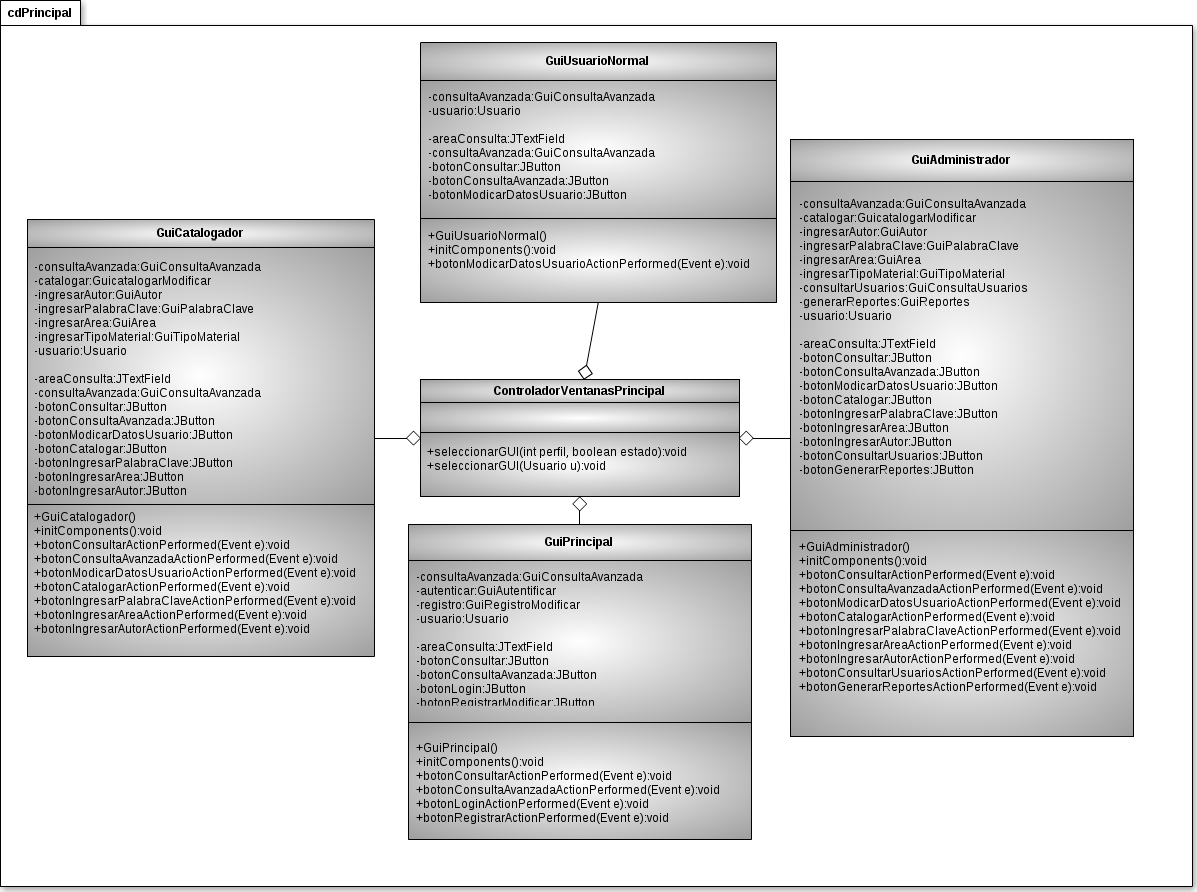
\includegraphics[width=17cm, height=19cm]{DiagramasClase/PRINCIPAL}
			\end{minipage}
		
			\begin{minipage}[c]{1\linewidth}
				\centering
				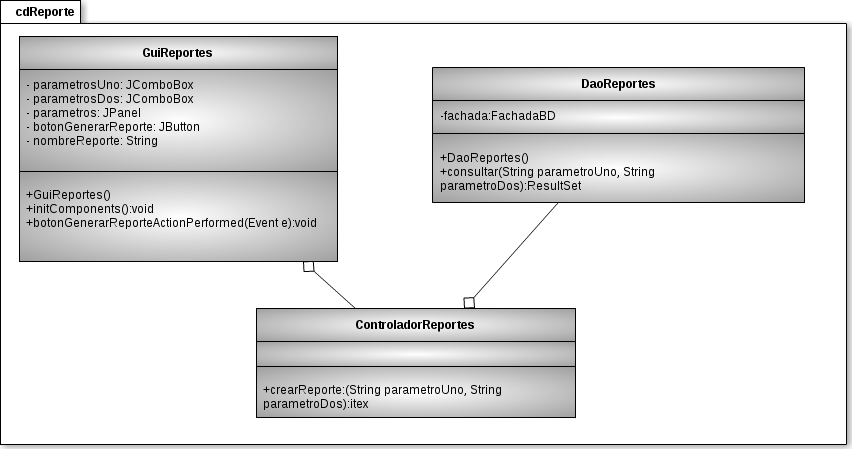
\includegraphics[scale=0.5]{DiagramasClase/Reporte}
			\end{minipage} \\[5cm]
		
			%fachada
			\begin{minipage}[c]{1\linewidth}
				\centering
				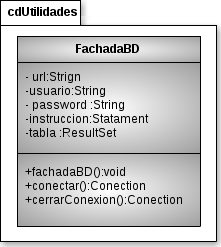
\includegraphics[scale=0.7]{DiagramasClase/Demas}
			\end{minipage}
		
			\begin{minipage}[c]{1\linewidth}
				\centering
				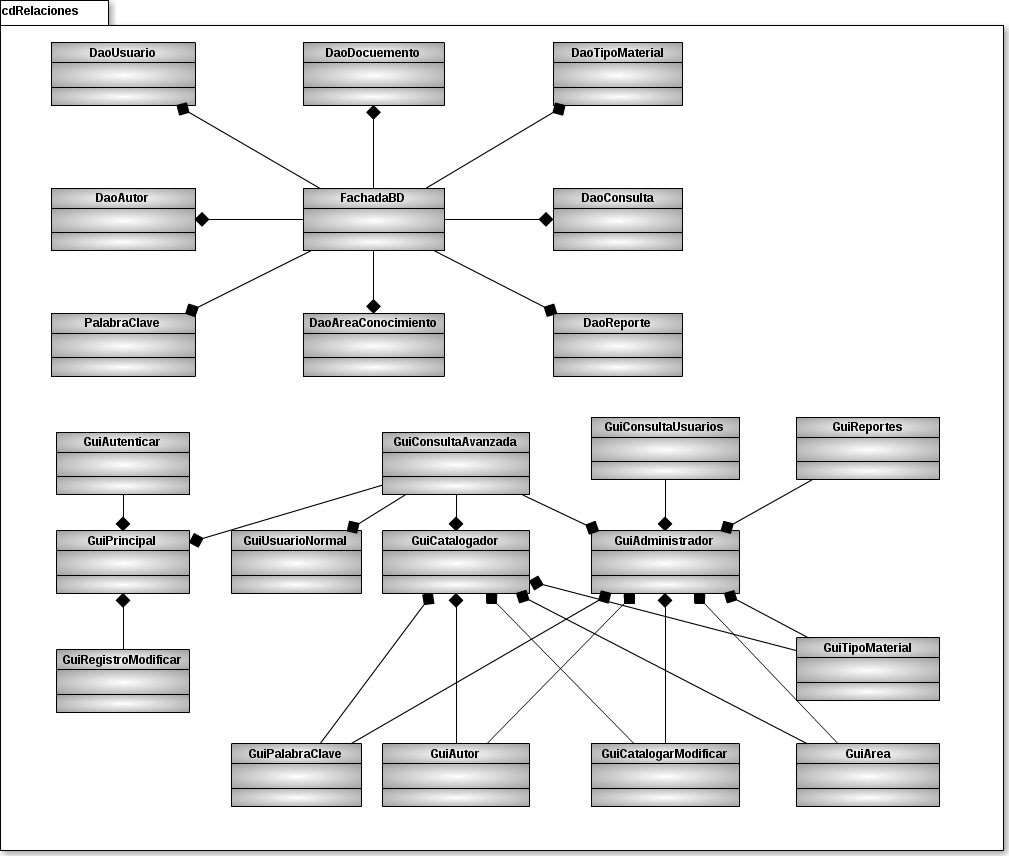
\includegraphics[width=17cm, height=18cm]{DiagramasClase/relaciones}
			\end{minipage}


		
		\subsection{Modelo ER} 
			\begin{minipage}[c]{1\linewidth}
                \centering
                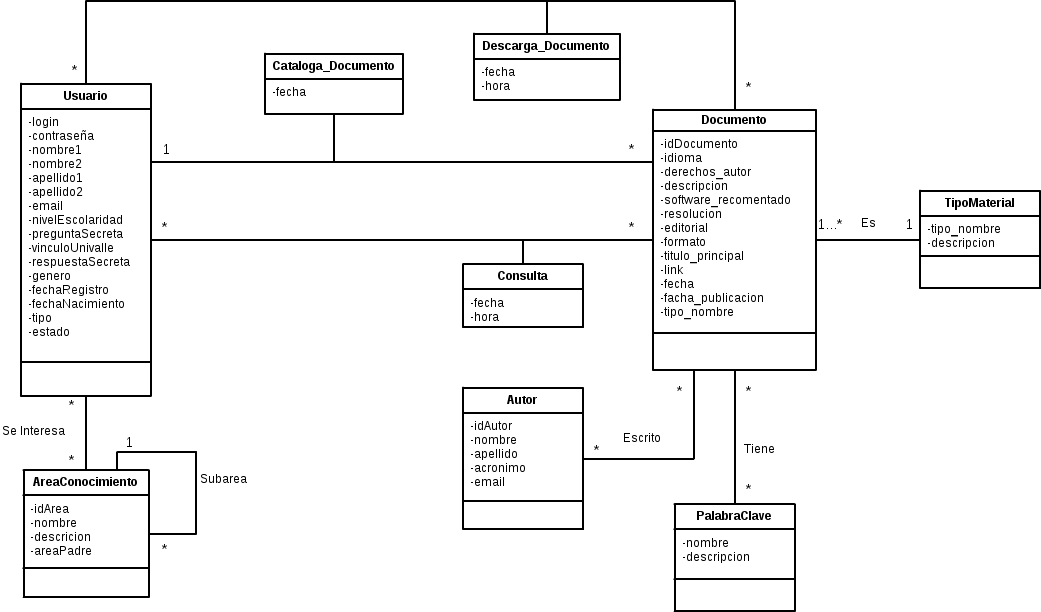
\includegraphics[width=16cm, height=14cm]{ModeloDatos}
        	\end{minipage}
                        
\section{Referencias}
        \begin{enumerate}
                \item Diseño de una plataforma experimental para la búsqueda y recuperación de
                documentos en una biblioteca digital PREDICA, Beatriz E. Florián, Maria E.
                Valencia, Paola J. Rodriguez, Marta Millán, Carlos M. Gaona, Javier E. Carrillo,
                Mauricio Ciprián. Revista Ingenieria y Competitividad, Volumen 9, No. 2, p
                93-104(2007)
                
                \item http://es.wikipedia.org/
                
                \item ITSM, Biblioteca Digital del Tecnológico de Monterrey: Documentos Tec,
                Ing. Miguel A. Arreola,Ing. Cuauhtemoc Durán, Ing. Alejandro Garza,
                Dr. David Garza, Lic. Rosa L. Gómez, Ing. Claudio Ramírez, Ing. Marta Sordia,
                Ing. Ramón E. Zayas. Abril de 1999                
                
                \item Especificación del proyecto.
        \end{enumerate}                
                        
\end{document}